% arXiv-style Lecture Notes -- Thuật Toán (Algorithms)
% Adapted from kourgeorge/arxiv-style (NeurIPS-based preprint template)
\documentclass[10pt]{article}

\usepackage{arxiv}

% XeLaTeX Unicode support
\usepackage{fontspec}
\setmonofont{Noto Sans Mono}

% Math
\usepackage{amsmath,amssymb,amsfonts}

% TikZ for Manning-style annotations
\usepackage{tikz}
\usetikzlibrary{tikzmark,calc,arrows.meta,decorations.pathreplacing,matrix,positioning}

% === ANIMATION ENVIRONMENTS (YouTube Style) ===
\newenvironment{sortanimation}[1][]{
  \begin{center}
  \begin{tikzpicture}[
    >=Stealth,
    arraynode/.style={draw, minimum width=2.2em, minimum height=2.2em, anchor=center, font=\sffamily},
    sorted/.style={arraynode, fill=green!15},
    pivot/.style={arraynode, fill=orange!30},
    compare/.style={arraynode, fill=blue!15, draw=blue!80!black, thick},
    normal/.style={arraynode, fill=white},
    #1
  ]
}{
  \end{tikzpicture}
  \end{center}
}

% Pseudocode styling
\usepackage{listings}
\usepackage[table]{xcolor}  % 'table' option loads colortbl for \cellcolor
\definecolor{codebg}{HTML}{F7F7F7}
\definecolor{codekw}{HTML}{0033B3}
\definecolor{codecomment}{HTML}{6A7F7F}
\definecolor{codestring}{HTML}{067D17}
\lstdefinestyle{pseudocode}{
  backgroundcolor=\color{codebg},
  basicstyle=\ttfamily\small,
  keywordstyle=\bfseries\color{codekw},
  commentstyle=\itshape\color{codecomment},
  stringstyle=\color{codestring},
  breaklines=true,
  frame=single,
  framerule=0.4pt,
  rulecolor=\color{gray!50},
  xleftmargin=6pt,
  xrightmargin=6pt,
  aboveskip=8pt,
  belowskip=6pt,
  columns=flexible,
  keepspaces=true,
  morekeywords={if,else,for,while,return,to,downto,and,or,not,in,do,end,then,swap,print},
  morecomment=[l]{//},
  morecomment=[s]{/*}{*/},
  literate={INF}{$\infty$}{1} {!=}{$\neq$}{1} {<=}{$\leq$}{1} {>=}{$\geq$}{1} {->}{$\to$}{1},
}
\lstset{style=pseudocode}

% Callout boxes for Intuition and Pitfall
\usepackage{tcolorbox}
\newcommand{\intuition}[1]{%
  \begin{tcolorbox}[colback=blue!5!white, colframe=blue!60!white, leftrule=3pt,
    toprule=0pt, bottomrule=0pt, rightrule=0pt,
    boxsep=2pt, left=6pt, right=6pt, top=4pt, bottom=4pt]
  \small\textbf{\textcolor{blue!80!black}{Trực giác: }}#1
  \end{tcolorbox}}
\newcommand{\pitfall}[1]{%
  \begin{tcolorbox}[colback=red!5!white, colframe=red!60!white, leftrule=3pt,
    toprule=0pt, bottomrule=0pt, rightrule=0pt,
    boxsep=2pt, left=6pt, right=6pt, top=4pt, bottom=4pt]
  \small\textbf{\textcolor{red!70!black}{Sai lầm thường gặp: }}#1
  \end{tcolorbox}}

% === PEDAGOGICAL ENVIRONMENTS ===
% Why? prompt -- Elaborative Interrogation
\newcommand{\whyprompt}[1]{%
  \begin{tcolorbox}[colback=yellow!8!white, colframe=orange!70!yellow, leftrule=3pt,
    toprule=0pt, bottomrule=0pt, rightrule=0pt,
    boxsep=2pt, left=6pt, right=6pt, top=4pt, bottom=4pt]
  {\small\textbf{\textcolor{orange!80!black}{$\boldsymbol{?}$ Tại sao? }} #1}
  \end{tcolorbox}}

% Trace It Yourself -- Active Processing
\newenvironment{traceyourself}[1]{%
  \begin{tcolorbox}[colback=green!5!white, colframe=green!60!black, leftrule=3pt,
    toprule=0pt, bottomrule=0pt, rightrule=0pt,
    boxsep=2pt, left=6pt, right=6pt, top=4pt, bottom=4pt,
    title={\small\textcolor{green!80!black}{$\triangleright$ Tự Trace: #1}}]
  \small
}{\end{tcolorbox}}

% Feynman Technique -- Explain in your own words
\newcommand{\feynman}[1]{%
  \begin{tcolorbox}[colback=violet!5!white, colframe=violet!60!white, leftrule=3pt,
    toprule=0pt, bottomrule=0pt, rightrule=0pt,
    boxsep=2pt, left=6pt, right=6pt, top=4pt, bottom=4pt]
  {\small\textbf{\textcolor{violet!80!black}{$\Rightarrow$ Giải thích bằng lời bạn: }} #1}
  \end{tcolorbox}}

% Checkpoint -- Quick self-check
\newcommand{\checkpoint}[1]{%
  \begin{tcolorbox}[colback=orange!5!white, colframe=orange!70!black, leftrule=3pt,
    toprule=0pt, bottomrule=0pt, rightrule=0pt,
    boxsep=2pt, left=6pt, right=6pt, top=4pt, bottom=4pt]
  {\small\textbf{\textcolor{orange!80!black}{$\checkmark$ Tự kiểm tra: }} #1}
  \end{tcolorbox}}

% Tables
\usepackage{longtable,booktabs,array}
\newcounter{none}
\usepackage{calc}
\usepackage{etoolbox}
\makeatletter
\patchcmd\longtable{\par}{\if@noskipsec\mbox{}\fi\par}{}{}
\makeatother

% Links
\usepackage[colorlinks=true,linkcolor=blue,citecolor=blue,urlcolor=blue]{hyperref}
\hypersetup{
  pdfauthor={Do Minh Phung},
  pdftitle={Lecture Notes -- Thuật Toán (Algorithms)},
  pdfsubject={Thuật toán, CLRS, Introduction to Algorithms},
  pdfkeywords={Algorithms, CLRS, Sorting, Graph, MST, Dijkstra, Dynamic Programming, NP-Complete, Do Minh Phung},
  pdfcreator={XeLaTeX},
}
\usepackage{bookmark}
\usepackage{capt-of}  % for \captionof outside float environments

% Utilities
\setlength{\emergencystretch}{3em}
\providecommand{\tightlist}{\setlength{\itemsep}{0pt}\setlength{\parskip}{0pt}}
\setcounter{secnumdepth}{3}  % numbered sections

% ===== arXiv metadata =====
\title{Lecture Notes -- Thuật Toán (Algorithms) \\
\large Theo phong cách CLRS (Introduction to Algorithms, 4th Ed.)}

\renewcommand{\undertitle}{}
\renewcommand{\headeright}{Lecture Notes: Thuật Toán}
\renewcommand{\shorttitle}{Thuật Toán -- Algorithms}

\author{
  Tổng hợp từ bài giảng Thuật Toán \\
  Semester 2025--2026 \\
  \texttt{Ngày tạo: 12/03/2026}
}

\date{}

\begin{document}
\maketitle

\begin{abstract}
Tài liệu tổng hợp toàn bộ kiến thức môn Thuật Toán theo phong cách sách \textit{Introduction to Algorithms} (CLRS, 4th Edition). Bao gồm: ký hiệu tiệm cận, sắp xếp (Insertion, Selection, Merge, Quick Sort), Master Theorem, lý thuyết đồ thị, Greedy \& MST (Kruskal, Prim), Dijkstra, quy hoạch động (Floyd-Warshall, nhân chuỗi ma trận), và P/NP/NP-Complete. Kèm theo bảng cheat sheet, template giải bài tập, và phụ lục tra cứu ký hiệu toán học.
\end{abstract}

\keywords{Thuật toán \and CLRS \and Sắp xếp \and Đồ thị \and MST \and Dijkstra \and Quy hoạch động \and NP-Complete}

\vspace{0.5cm}

% ===== HOW TO USE THIS DOCUMENT =====
\begin{tcolorbox}[colback=gray!5!white, colframe=gray!60!black,
  title={\textbf{\large Cách sử dụng tài liệu này -- Hệ thống tự học}},
  fonttitle=\bfseries, coltitle=white, colbacktitle=gray!70!black]

Tài liệu này không chỉ để đọc -- mà để \textbf{tương tác}. Bạn sẽ gặp 4 loại hộp đặc biệt:

\begin{itemize}
\tightlist
\item \textcolor{orange!80!black}{\textbf{Tại sao?}} -- Dừng lại và suy nghĩ trước khi đọc tiếp. Tự trả lời trước, rồi kiểm tra.
\item \textcolor{green!60!black}{\textbf{Tự Trace}} -- Lấy giấy bút, tự trace thuật toán bằng tay. \textbf{Đừng chỉ đọc!}
\item \textcolor{violet!80!black}{\textbf{Giải thích bằng lời bạn}} -- Thử giải thích như đang dạy bạn bè. Nếu bí = bạn chưa hiểu.
\item \textcolor{orange!80!black}{\textbf{Tự kiểm tra}} -- Câu hỏi nhanh. Trả lời trong đầu trước khi lật trang.
\end{itemize}
\end{tcolorbox}


\section*{KHUNG NHẬN DẠNG ĐỀ THI NHANH}\addcontentsline{toc}{section}{KHUNG NHẬN DẠNG ĐỀ THI NHANH}\label{khung-nhux1eadn-dux1ea1ng-ux111ux1ec1-thi-nhanh}

{\def\LTcaptype{none} % do not increment counter
\begin{longtable}[]{@{}
  >{\raggedright\arraybackslash}p{(\linewidth - 4\tabcolsep) * \real{0.3333}}
  >{\raggedright\arraybackslash}p{(\linewidth - 4\tabcolsep) * \real{0.3333}}
  >{\raggedright\arraybackslash}p{(\linewidth - 4\tabcolsep) * \real{0.3333}}@{}}
\toprule\noalign{}
\begin{minipage}[b]{\linewidth}\raggedright
Khi đề bài yêu cầu\ldots{}
\end{minipage} & \begin{minipage}[b]{\linewidth}\raggedright
Dùng kỹ thuật
\end{minipage} & \begin{minipage}[b]{\linewidth}\raggedright
Chương
\end{minipage} \\
\midrule\noalign{}
\endhead
\bottomrule\noalign{}
\endlastfoot
Sắp xếp mảng, so sánh thuật toán sort & \textbf{Sorting Algorithms} &
\hyperref[chux1b0ux1a1ng-2-thuux1eadt-touxe1n-sux1eafp-xux1ebfp-clrs-ch.2-7-8]{\textcolor{blue}{\underline{Ch.2}}} \\
Giải công thức đệ quy T(n) & \textbf{Master Theorem / Recursion Tree} &
\hyperref[chux1b0ux1a1ng-3-master-theorem-giux1ea3i-ux111ux1ec7-quy-clrs-ch.4]{\textcolor{blue}{\underline{Ch.3}}} \\
Biểu diễn đồ thị, danh sách kề, ma trận kề & \textbf{Graph
Representation} & \hyperref[chux1b0ux1a1ng-4-luxfd-thuyux1ebft-ux111ux1ed3-thux1ecb-clrs-ch.22]{\textcolor{blue}{\underline{Ch.4}}} \\
Tìm cây bao trùm nhỏ nhất (MST) & \textbf{Kruskal / Prim} & \hyperref[chux1b0ux1a1ng-5-greedy-mst-clrs-ch.16-23]{\textcolor{blue}{\underline{Ch.5}}} \\
Tìm đường đi ngắn nhất từ 1 đỉnh & \textbf{Dijkstra} & \hyperref[chux1b0ux1a1ng-6-ux111ux1b0ux1eddng-ux111i-ngux1eafn-nhux1ea5t-dijkstra-clrs-ch.24]{\textcolor{blue}{\underline{Ch.6}}} \\
Tìm đường đi ngắn nhất mọi cặp đỉnh & \textbf{Floyd-Warshall} & \hyperref[chux1b0ux1a1ng-7-quy-houx1ea1ch-ux111ux1ed9ng-dp-clrs-ch.14]{\textcolor{blue}{\underline{Ch.7}}} \\
Tính Fibonacci, tổ hợp C(n,k) & \textbf{Dynamic Programming} & \hyperref[chux1b0ux1a1ng-7-quy-houx1ea1ch-ux111ux1ed9ng-dp-clrs-ch.14]{\textcolor{blue}{\underline{Ch.7}}} \\
Nhân chuỗi ma trận tối ưu & \textbf{Matrix Chain Multiplication} &
\hyperref[chux1b0ux1a1ng-8-nhuxe2n-chuux1ed7i-ma-trux1eadn-clrs-14.2]{\textcolor{blue}{\underline{Ch.8}}} \\
Chứng minh bài toán NP-Complete & \textbf{P, NP, NP-Complete} & \hyperref[chux1b0ux1a1ng-9-p-np-np-complete-clrs-ch.34]{\textcolor{blue}{\underline{Ch.9}}} \\
\end{longtable}
}
\captionof{table}{Khung nhận dạng đề thi nhanh -- Quick Exam Pattern Recognition}\label{tab:khung-nhan-dang}

\begin{center}\rule{0.5\linewidth}{0.5pt}\end{center}

\section{Chương 1: Nền tảng -- Foundations (CLRS Ch.1--3)}\label{chux1b0ux1a1ng-1-nux1ec1n-tux1ea3ng-foundations-clrs-ch.1-3}

\intuition{Trước khi viết 1 dòng code, cần có ngôn ngữ chung để \textbf{so sánh} hiệu quả thuật toán -- đó là ký hiệu tiệm cận ($O$, $\Theta$, $\Omega$). Cũng cần công cụ \textbf{chứng minh đúng} -- đó là Loop Invariant. Fibonacci là bài toán mẫu để thấy sức mạnh của DP so với đệ quy ngây thơ.}

\subsection{1.1 Thuật toán là gì?}\label{thuux1eadt-touxe1n-luxe0-guxec}

\textbf{Định nghĩa (CLRS):} Thuật toán là một thủ tục tính toán xác định
rõ ràng, nhận \textbf{input} và cho ra \textbf{output}, giải quyết một
\textbf{bài toán tính toán} cụ thể.

\textbf{Tính đúng đắn (Correctness):} Thuật toán \textbf{đúng} nếu với
\textbf{mọi} input hợp lệ, nó \textbf{dừng} và cho ra output đúng.

\subsection{1.2 Ký hiệu tiệm cận (Asymptotic Notation) -- CLRS
Ch.3}\label{kuxfd-hiux1ec7u-tiux1ec7m-cux1eadn-asymptotic-notation-clrs-ch.3}

\subsubsection{Định nghĩa chính
xác:}\label{ux111ux1ecbnh-nghux129a-chuxednh-xuxe1c}

\textbf{\(\Theta\) (Theta) -- Chặn chặt:}

\(f(n) = \Theta(g(n)) \Leftrightarrow \exists\, c_1, c_2 > 0,\, n_0\)
sao cho \(\forall n \geq n_0\):
\[c_1 \cdot g(n) \leq f(n) \leq c_2 \cdot g(n)\]

\textbf{\(O\) (Big-O) -- Chặn trên:}

\(f(n) = O(g(n)) \Leftrightarrow \exists\, c > 0,\, n_0\) sao cho
\(\forall n \geq n_0\): \[f(n) \leq c \cdot g(n)\]

\textbf{\(\Omega\) (Omega) -- Chặn dưới:}

\(f(n) = \Omega(g(n)) \Leftrightarrow \exists\, c > 0,\, n_0\) sao cho
\(\forall n \geq n_0\): \[f(n) \geq c \cdot g(n)\]

\textbf{\(o\) (little-o) -- Chặn trên không chặt:}

\(f(n) = o(g(n)) \Leftrightarrow \lim_{n \to \infty} f(n)/g(n) = 0\)

\textbf{\(\omega\) (little-omega) -- Chặn dưới không chặt:}

\(f(n) = \omega(g(n)) \Leftrightarrow \lim_{n \to \infty} f(n)/g(n) = \infty\)

\subsubsection{Quan hệ:}\label{quan-hux1ec7}

\(f(n) = \Theta(g(n)) \Leftrightarrow f(n) = O(g(n))\) \textbf{VÀ}
\(f(n) = \Omega(g(n))\)

\subsubsection{Ví dụ:}\label{vuxed-dux1ee5}

\begin{itemize}
\tightlist
\item
  \(2n^2 + 3n + 1 = \Theta(n^2)\) -- chọn \(c_1=2, c_2=6, n_0=1\)
\item
  \(n \lg n = O(n^2)\) -- vì \(n \lg n \leq n^2\) với \(n \geq 1\)
\item
  \(n^3 = \Omega(n^2)\) -- vì \(n^3 \geq n^2\) với \(n \geq 1\)
\end{itemize}

\whyprompt{Tại sao ta không dùng \textbf{đo thời gian chạy thực tế} (empirical timing) thay cho Big-O? Gợi ý: nghĩ về sự khác nhau giữa các máy tính, kích thước input, và tính phổ quát (generality).}

\feynman{Giải thích sự khác biệt giữa $O$, $\Theta$, và $\Omega$ cho một người bạn không học CS. Dùng ví dụ thực tế (tốc độ xe, giá cả...). Nếu bạn không giải thích được $\Theta$ = ``chặn chặt'' nghĩa là gì -- bạn chưa thực sự hiểu.}

\subsection{1.2a Cách ước lượng Complexity từ Pseudocode}\label{cach-uoc-luong}

\intuition{Nhìn pseudocode, ta ``đếm'' số phép toán cơ bản (so sánh, gán, cộng) theo kích thước input $n$. Không cần đếm chính xác -- chỉ cần xác định \textbf{bậc tăng trưởng} (growth rate). Dưới đây là các quy tắc nhanh giúp ước lượng ngay từ cấu trúc code.}

\subsubsection{Quy tắc ước lượng Time Complexity:}

\begin{enumerate}
\item \textbf{Câu lệnh đơn} (gán, so sánh, return): $\Theta(1)$ -- hằng số.

\item \textbf{Vòng lặp đơn} \texttt{for i = 1 to n}: thân vòng chạy $n$ lần $\to$ $\Theta(n)$.

\item \textbf{Vòng lặp lồng nhau} (nested loops):
\begin{itemize}
\item 2 vòng \texttt{for} lồng nhau, mỗi vòng $n$ lần $\to$ $n \times n = \Theta(n^2)$. \textit{(Bubble Sort, Selection Sort)}
\item 3 vòng lồng $\to$ $\Theta(n^3)$. \textit{(Floyd-Warshall, Matrix Chain)}
\end{itemize}

\item \textbf{Vòng lặp chia đôi} \texttt{while n > 1: n = n/2}: chạy $\lg n$ lần $\to$ $\Theta(\lg n)$. \textit{(Binary Search)}

\item \textbf{Đệ quy chia đôi + gộp tuyến tính:}\\
$T(n) = 2T(n/2) + \Theta(n)$ $\to$ $\Theta(n \lg n)$. \textit{(Merge Sort)}\\
Dùng \textbf{Master Theorem} (Chương 3) hoặc \textbf{Recursion Tree} để giải.

\item \textbf{Đệ quy phân nhánh đầy đủ:}\\
$T(n) = 2T(n-1) + \Theta(1)$ $\to$ $\Theta(2^n)$. \textit{(Fibonacci naive)}
\end{enumerate}

\begin{tcolorbox}[colback=blue!3, colframe=blue!40, boxrule=0.5pt, arc=2pt, title={\small\textbf{Bảng tra nhanh: Cấu trúc code $\to$ Complexity}}]
\begin{tabular}{|l|l|l|}
\hline
\textbf{Cấu trúc Pseudocode} & \textbf{Time} & \textbf{Ví dụ} \\
\hline
1 vòng \texttt{for} ($1$ đến $n$) & $\Theta(n)$ & Tìm max \\
\hline
2 vòng \texttt{for} lồng nhau & $\Theta(n^2)$ & Bubble Sort \\
\hline
3 vòng \texttt{for} lồng nhau & $\Theta(n^3)$ & Floyd-Warshall \\
\hline
\texttt{while n = n/2} & $\Theta(\lg n)$ & Binary Search \\
\hline
$T(n)=2T(n/2)+\Theta(n)$ & $\Theta(n\lg n)$ & Merge Sort \\
\hline
$T(n)=T(n-1)+\Theta(n)$ & $\Theta(n^2)$ & Quick Sort (worst) \\
\hline
$T(n)=2T(n-1)+\Theta(1)$ & $\Theta(2^n)$ & Fibonacci (naive) \\
\hline
\end{tabular}
\end{tcolorbox}

\subsubsection{Quy tắc ước lượng Space Complexity:}

\begin{enumerate}
\item \textbf{Biến đơn} ($i$, $j$, $key$): $O(1)$ -- không phụ thuộc $n$.
\item \textbf{Mảng phụ} kích thước $n$ (ví dụ: mảng tạm trong Merge): $\Theta(n)$.
\item \textbf{Stack đệ quy:} Mỗi lần gọi đệ quy chiếm $O(1)$ stack frame. Chiều sâu đệ quy $d$ $\to$ $O(d)$ space.
\begin{itemize}
\item Merge Sort: sâu $\lg n$ tầng + mảng tạm $\Theta(n)$ $\to$ $\Theta(n)$.
\item Quick Sort: sâu $\lg n$ (avg) hoặc $n$ (worst) $\to$ $O(\lg n)$ đến $O(n)$.
\end{itemize}
\item \textbf{Ma trận} $n \times n$: $\Theta(n^2)$. \textit{(Floyd-Warshall: ma trận $D$)}
\end{enumerate}

\subsection{1.2b Độ phức tạp không gian (Space Complexity)}\label{space-complexity}

\intuition{Time Complexity hỏi ``mất \textbf{bao lâu}?''. Space Complexity hỏi ``tốn \textbf{bao nhiêu bộ nhớ}?''. Trong thực tế, bộ nhớ thường là tài nguyên \textbf{hữu hạn hơn} thời gian -- bạn có thể chờ lâu hơn, nhưng không thể mua thêm RAM giữa lúc chạy. Hiểu space complexity giúp chọn đúng thuật toán cho bài toán lớn.}

\subsubsection{Hai loại bộ nhớ cần phân biệt:}

\begin{enumerate}
\def\labelenumi{\arabic{enumi}.}
\tightlist
\item
  \textbf{Auxiliary Space (Bộ nhớ phụ):} Bộ nhớ \textbf{thêm} ngoài input. Ví dụ: mảng tạm trong Merge Sort.
\item
  \textbf{Total Space:} Auxiliary + Input. Ví dụ: ma trận $D[n \times n]$ trong Floyd-Warshall là \textit{cả} output lẫn workspace.
\end{enumerate}

\begin{quote}
Khi nói ``Space Complexity = $O(n)$'' thường ám chỉ \textbf{auxiliary space}, trừ khi nói rõ.
\end{quote}

\subsubsection{In-place là gì?}

\textbf{In-place} = thuật toán \textbf{chỉ dùng $O(1)$ hoặc $O(\lg n)$ bộ nhớ phụ}, tức chỉnh sửa trực tiếp trên input mà không tạo bản sao lớn.

\begin{itemize}
\tightlist
\item In-place: Insertion Sort, Quick Sort, Selection Sort
\item \textbf{Not} in-place: Merge Sort (cần mảng tạm $\Theta(n)$)
\end{itemize}

\subsubsection{Stack Space cho đệ quy:}

Mỗi lần gọi đệ quy tạo \textbf{stack frame} mới trên bộ nhớ. Thuật toán đệ quy sâu $d$ mức tiêu tốn $O(d)$ stack space.

\begin{itemize}
\tightlist
\item Quick Sort: chiều sâu trung bình $O(\lg n)$, worst case $O(n)$ \quad (nên Random + tail-call optimization)
\item Merge Sort: luôn $O(\lg n)$ chiều sâu, nhưng cần $\Theta(n)$ mảng phụ bên ngoài
\item Fibonacci đệ quy: chiều sâu $O(n)$ $\to$ stack space $O(n)$; DP bottom-up chỉ $O(1)$
\end{itemize}

\subsubsection{Bảng Space Complexity chi tiết:}\label{bang-space-complexity}

\begin{quote}
\textbf{Lưu ý thuật ngữ -- Auxiliary (Bộ nhớ phụ):} Cột này chỉ đánh giá lượng bộ nhớ \textit{sinh thêm} trong quá trình chạy (biến tạm, mảng copy, dung lượng ngăn xếp đệ quy...), \textbf{hoàn toàn không tính} tới kích thước lưu trữ của bản thân dữ liệu Input ($V, E, n$). Điều này giúp ta thấy rõ chi phí thực sự dội lên bộ nhớ của từng thuật toán.
\end{quote}

{\def\LTcaptype{none}
\begin{longtable}[]{@{}
  >{\raggedright\arraybackslash}p{(\linewidth - 6\tabcolsep) * \real{0.2200}}
  >{\raggedright\arraybackslash}p{(\linewidth - 6\tabcolsep) * \real{0.1500}}
  >{\raggedright\arraybackslash}p{(\linewidth - 6\tabcolsep) * \real{0.1300}}
  >{\raggedright\arraybackslash}p{(\linewidth - 6\tabcolsep) * \real{0.5000}}@{}}
\toprule\noalign{}
\begin{minipage}[b]{\linewidth}\raggedright
Thuật toán
\end{minipage} & \begin{minipage}[b]{\linewidth}\raggedright
Auxiliary
\end{minipage} & \begin{minipage}[b]{\linewidth}\raggedright
In-place?
\end{minipage} & \begin{minipage}[b]{\linewidth}\raggedright
Tại sao?
\end{minipage} \\
\midrule\noalign{}
\endhead
\bottomrule\noalign{}
\endlastfoot
Insertion Sort & $O(1)$ & Có & Chỉ dùng biến \texttt{key}, \texttt{i} -- dịch phần tử trên chính mảng \\
Selection Sort & $O(1)$ & Có & Chỉ dùng biến \texttt{min}, \texttt{i}, \texttt{j} -- swap trên chính mảng \\
Merge Sort & $\Theta(n)$ & \textbf{Không} & Hàm Merge tạo mảng tạm $L[1..n_1]$, $R[1..n_2]$ để trộn \\
Quick Sort & $O(\lg n)$ avg & Có & Partition chỉ swap trên mảng. $O(\lg n)$: stack đệ quy \\
Kruskal & $O(V)$ & -- & Union-Find: mảng parent[] + rank[] cho $V$ đỉnh \\
Prim & $O(V)$ & -- & Priority queue cho $V$ đỉnh: key[] + $\pi$[] \\
Dijkstra & $O(V)$ & -- & Mảng $d[V]$, $\pi[V]$, priority queue $Q$ \\
Floyd-Warshall & $\Theta(V^2)$ & -- & Ma trận $D[V \times V]$ lưu khoảng cách \\
MCM & $\Theta(n^2)$ & -- & Bảng $m[n \times n]$ + $s[n \times n]$ \\
Pascal $C(n,k)$ v1 & $O(nk)$ & -- & Bảng 2D $C[0..n][0..k]$ \\
Pascal $C(n,k)$ v2 & $O(k)$ & -- & Chỉ dùng 1 hàng $C[0..k]$, cập nhật \textbf{ngược} \\
Fibonacci DP & $O(1)$ & -- & Chỉ lưu $a$, $b$, $c$ (3 biến) \\
Fibonacci Matrix & $O(1)$ & -- & Ma trận $2 \times 2$ cố định \\
\end{longtable}
}
\captionof{table}{So sánh Space Complexity chi tiết các thuật toán sắp xếp}\label{tab:space-complexity}

\whyprompt{Tại sao Merge Sort cần $\Theta(n)$ extra space mà Quick Sort thì không? Gợi ý: nghĩ về cách Merge gộp 2 mảng con -- có thể merge ``tại chỗ'' (in-place) không? Nếu có, tại sao thực tế không ai làm vậy?}

\checkpoint{Quick Sort có phải ``in-place'' hoàn toàn không? Hay vẫn tốn bộ nhớ? (Gợi ý: nghĩ về stack đệ quy.) Worst case stack depth của Quick Sort là bao nhiêu? Làm sao tránh?}

\subsection{\texorpdfstring{Chứng minh tính đúng đắn -- Loop
Invariant (CLRS
\S 2.1)}{Chứng minh tính đúng đắn -- Loop Invariant (CLRS 2.1)}}\label{chux1ee9ng-minh-tuxednh-ux111uxfang-ux111ux1eafn-loop-invariant-clrs-2.1}

\subsubsection{Ba bước chứng
minh:}\label{ba-bux1b0ux1edbc-chux1ee9ng-minh}

\begin{enumerate}
\def\labelenumi{\arabic{enumi}.}
\tightlist
\item
  \textbf{Initialization (Khởi tạo):} Bất biến đúng \textbf{trước lần
  lặp đầu tiên}
\item
  \textbf{Maintenance (Duy trì):} Nếu đúng trước lần lặp thứ \(i\)
  \(\to\) đúng trước lần lặp thứ \(i+1\)
\item
  \textbf{Termination (Kết thúc):} Khi vòng lặp dừng, bất biến + điều
  kiện dừng \(\to\) \textbf{kết quả đúng}
\end{enumerate}

\begin{quote}
Tương tự \textbf{quy nạp toán học}, nhưng có bước dừng \(\to\) cho kết
luận hữu ích.
\end{quote}

\begin{traceyourself}{Loop Invariant -- Điền 3 bước}
Hãy tự chứng minh Insertion Sort đúng bằng Loop Invariant. Điền vào:

\textbf{1. Bất biến:} ``Tại đầu mỗi lần lặp for với $j$, \underline{\hspace{8cm}}''

\textbf{2. Initialization ($j=$ \underline{\hspace{1cm}}):} \underline{\hspace{10cm}}

\textbf{3. Maintenance:} Giả sử đúng trước lần $j$, chứng minh đúng trước lần $j+1$:

\underline{\hspace{12cm}}

\textbf{4. Termination:} Vòng lặp dừng khi $j =$ \underline{\hspace{2cm}}. Kết luận: \underline{\hspace{6cm}}

\textit{(So sánh với phần 1.3 ở trên sau khi hoàn thành.)}
\end{traceyourself}

\subsection{1.4 Fibonacci -- Bốn cách tiếp cận (CLRS Problem 31-3
style)}\label{fibonacci-bux1ed1n-cuxe1ch-tiux1ebfp-cux1eadn-clrs-problem-31-3-style}

\subsubsection{\texorpdfstring{Cách 1: Đệ quy --
\(O(2^n)\)}{Cách 1: Đệ quy -- O(2\^{}n)}}\label{cuxe1ch-1-ux111ux1ec7-quy-o2n}

\begin{tcolorbox}[colback=gray!8, colframe=gray!50, boxrule=0.5pt, arc=2pt,
  left=6pt, right=6pt, top=4pt, bottom=4pt,
  title={\small\textbf{Pseudocode 1: Fibonacci -- Đệ quy}}]
\begin{verbatim}
Fib(n):
    if n <= 1: return n
    return Fib(n-1) + Fib(n-2)
\end{verbatim}
\end{tcolorbox}

\begin{tcolorbox}[colback=yellow!5, colframe=orange!50, boxrule=0.5pt, arc=2pt, title={\small\textbf{Phân tích Complexity -- Fibonacci Đệ quy}}]
\begin{tabular}{|l|l|l|}
\hline
\textbf{Dòng code} & \textbf{Số lần chạy} & \textbf{Chi phí} \\
\hline
\texttt{if n <= 1: return n} & $\Theta(1)$ & base case \\
\hline
\texttt{return Fib(n-1) + Fib(n-2)} & $T(n-1)+T(n-2)$ & 2 nhánh đệ quy \\
\hline
\end{tabular}
\vspace{0.2cm}

\textbf{Recurrence:} $T(n) = T(n-1) + T(n-2) + \Theta(1)$.\\
\textbf{Time:} Cây đệ quy có $\sim 2^n$ nút (thực tế $\Theta(\varphi^n)$ với $\varphi\approx1.618$) $\to$ \textbf{exponential}.\\
\textbf{Space:} Chiều sâu cây = $n$ $\to$ stack đệ quy $O(n)$.
\end{tcolorbox}

\begin{tcolorbox}[colback=yellow!5, colframe=orange!50, boxrule=0.5pt, arc=2pt, title={\small\textbf{Phân tích Complexity -- Fibonacci Đệ quy}}]
\begin{tabular}{|l|l|l|}
\hline
\textbf{Dòng code} & \textbf{Số lần chạy} & \textbf{Chi phí} \\
\hline
\texttt{if n <= 1: return n} & $\Theta(1)$ & base case \\
\hline
\texttt{return Fib(n-1) + Fib(n-2)} & $T(n-1)+T(n-2)$ & 2 nhánh đệ quy \\
\hline
\end{tabular}
\vspace{0.2cm}

\textbf{Recurrence:} $T(n) = T(n-1) + T(n-2) + \Theta(1)$.\\
\textbf{Time:} Cây đệ quy có $\sim 2^n$ nút (thực tế $\Theta(\varphi^n)$ với $\varphi\approx1.618$) $\to$ \textbf{exponential}.\\
\textbf{Space:} Chiều sâu cây = $n$ $\to$ stack đệ quy $O(n)$.
\end{tcolorbox}

\textbf{Phân tích (CLRS style):} \(T(n) = T(n-1) + T(n-2) + \Theta(1)\).
Cây đệ quy có \(\sim 2^n\) nút \(\to\) \(T(n) = \Theta(\varphi^n)\) với
\(\varphi = (1+\sqrt{5})/2 \approx 1.618\) (tỷ lệ vàng).

\subsubsection{\texorpdfstring{Cách 2: DP Bottom-up -- \(O(n)\) time,
\(O(n)\)
space}{Cách 2: DP Bottom-up -- O(n) time, O(n) space}}\label{cuxe1ch-2-dp-bottom-up-on-time-on-space}

\begin{tcolorbox}[colback=gray!8, colframe=gray!50, boxrule=0.5pt, arc=2pt,
  left=6pt, right=6pt, top=4pt, bottom=4pt,
  title={\small\textbf{Pseudocode 2: Fibonacci -- DP Bottom-up}}]
\begin{verbatim}
Fib2(n):
    F[0] = 0, F[1] = 1
    for i = 2 to n:
        F[i] = F[i-1] + F[i-2]
    return F[n]
\end{verbatim}
\end{tcolorbox}

\begin{tcolorbox}[colback=yellow!5, colframe=orange!50, boxrule=0.5pt, arc=2pt, title={\small\textbf{Phân tích Complexity -- Fibonacci DP Bottom-up}}]
\begin{tabular}{|l|l|l|}
\hline
\textbf{Dòng code} & \textbf{Số lần chạy} & \textbf{Chi phí} \\
\hline
\texttt{F[0]=0, F[1]=1} & $2$ & $\Theta(1)$ khởi tạo \\
\hline
\texttt{for i = 2 to n} & $n-1$ & 1 vòng lặp \\
\hline
\quad \texttt{F[i] = F[i-1] + F[i-2]} & $n-1$ & $\Theta(1)$ mỗi lần \\
\hline
\texttt{return F[n]} & $1$ & $\Theta(1)$ \\
\hline
\end{tabular}
\vspace{0.2cm}

\textbf{Time:} 1 vòng \texttt{for} chạy $n-1$ lần $\to$ $\Theta(n)$. \textit{Nhanh gấp cấp số mũ so với đệ quy!}\\
\textbf{Space:} Mảng $F[0..n]$ có $n+1$ phần tử $\to$ $\Theta(n)$.
\end{tcolorbox}

\begin{tcolorbox}[colback=yellow!5, colframe=orange!50, boxrule=0.5pt, arc=2pt, title={\small\textbf{Phân tích Complexity -- Fibonacci DP Bottom-up}}]
\begin{tabular}{|l|l|l|}
\hline
\textbf{Dòng code} & \textbf{Số lần chạy} & \textbf{Chi phí} \\
\hline
\texttt{F[0]=0, F[1]=1} & $2$ & $\Theta(1)$ khởi tạo \\
\hline
\texttt{for i = 2 to n} & $n-1$ & 1 vòng lặp \\
\hline
\quad \texttt{F[i] = F[i-1] + F[i-2]} & $n-1$ & $\Theta(1)$ mỗi lần \\
\hline
\texttt{return F[n]} & $1$ & $\Theta(1)$ \\
\hline
\end{tabular}
\vspace{0.2cm}

\textbf{Time:} 1 vòng \texttt{for} chạy $n-1$ lần $\to$ $\Theta(n)$. \textit{Nhanh gấp cấp số mũ so với đệ quy!}\\
\textbf{Space:} Mảng $F[0..n]$ có $n+1$ phần tử $\to$ $\Theta(n)$.
\end{tcolorbox}

\textbf{Tại sao nhanh hơn?} Mỗi bài toán con \(F[i]\) chỉ tính \textbf{1
lần} \(\to\) tổng \(\Theta(n)\) phép cộng.

\subsubsection{\texorpdfstring{Cách 3: DP tối ưu space -- \(O(n)\) time,
\(O(1)\)
space}{Cách 3: DP tối ưu space -- O(n) time, O(1) space}}\label{cuxe1ch-3-dp-tux1ed1i-ux1b0u-space-on-time-o1-space}

\begin{tcolorbox}[colback=gray!8, colframe=gray!50, boxrule=0.5pt, arc=2pt,
  left=6pt, right=6pt, top=4pt, bottom=4pt,
  title={\small\textbf{Pseudocode 3: Fibonacci -- DP tối ưu space}}]
\begin{verbatim}
Fib3(n):
    if n <= 1: return n
    a := 0, b := 1
    for i = 2 to n:
        c := a + b; a := b; b := c
    return c
\end{verbatim}
\end{tcolorbox}

\begin{tcolorbox}[colback=yellow!5, colframe=orange!50, boxrule=0.5pt, arc=2pt, title={\small\textbf{Phân tích Complexity -- Fibonacci DP tối ưu space}}]
\begin{tabular}{|l|l|l|}
\hline
\textbf{Dòng code} & \textbf{Số lần chạy} & \textbf{Chi phí} \\
\hline
\texttt{a := 0, b := 1} & $2$ & $\Theta(1)$ khởi tạo \\
\hline
\texttt{for i = 2 to n} & $n-1$ & 1 vòng lặp \\
\hline
\quad \texttt{c:=a+b; a:=b; b:=c} & $n-1$ & $\Theta(1)$ mỗi lần \\
\hline
\texttt{return c} & $1$ & $\Theta(1)$ \\
\hline
\end{tabular}
\vspace{0.2cm}

\textbf{Time:} Giống cách 2: 1 vòng \texttt{for} $\to$ $\Theta(n)$.\\
\textbf{Space:} Chỉ dùng 3 biến $a, b, c$ $\to$ $O(1)$! \textit{Tối ưu hơn cách 2 (từ $\Theta(n)$ xuống $O(1)$).}
\end{tcolorbox}

\begin{tcolorbox}[colback=yellow!5, colframe=orange!50, boxrule=0.5pt, arc=2pt, title={\small\textbf{Phân tích Complexity -- Fibonacci DP tối ưu space}}]
\begin{tabular}{|l|l|l|}
\hline
\textbf{Dòng code} & \textbf{Số lần chạy} & \textbf{Chi phí} \\
\hline
\texttt{a := 0, b := 1} & $2$ & $\Theta(1)$ khởi tạo \\
\hline
\texttt{for i = 2 to n} & $n-1$ & 1 vòng lặp \\
\hline
\quad \texttt{c:=a+b; a:=b; b:=c} & $n-1$ & $\Theta(1)$ mỗi lần \\
\hline
\texttt{return c} & $1$ & $\Theta(1)$ \\
\hline
\end{tabular}
\vspace{0.2cm}

\textbf{Time:} Giống cách 2: 1 vòng \texttt{for} $\to$ $\Theta(n)$.\\
\textbf{Space:} Chỉ dùng 3 biến $a, b, c$ $\to$ $O(1)$! \textit{Tối ưu hơn cách 2 (từ $\Theta(n)$ xuống $O(1)$).}
\end{tcolorbox}

\subsubsection{\texorpdfstring{Cách 4: Lũy thừa ma trận --
\(O(\lg n)\)}{Cách 4: Lũy thừa ma trận -- O(\textbackslash log n)}}\label{cuxe1ch-4-lux169y-thux1eeba-ma-trux1eadn-olog-n}

Dựa trên công thức:
\[\begin{pmatrix} F(n+1) & F(n) \\ F(n) & F(n-1) \end{pmatrix} = \begin{pmatrix} 1 & 1 \\ 1 & 0 \end{pmatrix}^n\]
Dùng \textbf{repeated squaring} (CLRS \S 31.6): tính \(A^n\) bằng cách
bình phương liên tiếp \(\to\) \(O(\lg n)\) phép nhân ma trận
\(2 \times 2\).

\begin{center}\rule{0.5\linewidth}{0.5pt}\end{center}

\section{Chương 2: Thuật toán Sắp xếp -- Sorting Algorithms (CLRS Ch.2, 7, 8)}\label{chux1b0ux1a1ng-2-thuux1eadt-touxe1n-sux1eafp-xux1ebfp-clrs-ch.2-7-8}

\intuition{Sắp xếp là bài toán nền tảng nhất của CS. Chúng ta học 4 thuật toán không phải để nhớ code, mà để hiểu \textbf{3 mô hình thiết kế}: (1) Incremental (Insertion Sort), (2) Divide \& Conquer (Merge/Quick Sort), và (3) giới hạn lý thuyết $\Omega(n \lg n)$. Trong thực tế, Quick Sort \textbf{nhanh nhất} dù worst case $\Theta(n^2)$, vì pivot ngẫu nhiên hiếm khi xấu.}

\pitfall{(1) Nhầm worst case của Quick Sort với average case -- trong thực tế dùng randomized nên average $\Theta(n \lg n)$. (2) Merge Sort cần thêm $O(n)$ bộ nhớ -- không phải in-place. (3) Selection Sort tuy $O(n^2)$ nhưng không stable -- không thể dùng khi thứ tự relative quan trọng.}

\subsection{2.1 Bảng tổng hợp}\label{bux1ea3ng-tux1ed5ng-hux1ee3p}

{\def\LTcaptype{none} % do not increment counter
\begin{longtable}[]{@{}
  >{\raggedright\arraybackslash}p{(\linewidth - 12\tabcolsep) * \real{0.1429}}
  >{\raggedright\arraybackslash}p{(\linewidth - 12\tabcolsep) * \real{0.1429}}
  >{\raggedright\arraybackslash}p{(\linewidth - 12\tabcolsep) * \real{0.1429}}
  >{\raggedright\arraybackslash}p{(\linewidth - 12\tabcolsep) * \real{0.1429}}
  >{\raggedright\arraybackslash}p{(\linewidth - 12\tabcolsep) * \real{0.1429}}
  >{\raggedright\arraybackslash}p{(\linewidth - 12\tabcolsep) * \real{0.1429}}
  >{\raggedright\arraybackslash}p{(\linewidth - 12\tabcolsep) * \real{0.1429}}@{}}
\toprule\noalign{}
\begin{minipage}[b]{\linewidth}\raggedright
Thuật toán
\end{minipage} & \begin{minipage}[b]{\linewidth}\raggedright
Time Best
\end{minipage} & \begin{minipage}[b]{\linewidth}\raggedright
Time Avg
\end{minipage} & \begin{minipage}[b]{\linewidth}\raggedright
Time Worst
\end{minipage} & \begin{minipage}[b]{\linewidth}\raggedright
Space
\end{minipage} & \begin{minipage}[b]{\linewidth}\raggedright
Stable
\end{minipage} & \begin{minipage}[b]{\linewidth}\raggedright
In-place
\end{minipage} \\
\midrule\noalign{}
\endhead
\bottomrule\noalign{}
\endlastfoot
Bubble Sort & \(\Theta(n)\) & \(\Theta(n^2)\) & \(\Theta(n^2)\) &
\(O(1)\) & Yes & Yes \\
Selection Sort & \(\Theta(n^2)\) & \(\Theta(n^2)\) & \(\Theta(n^2)\) &
\(O(1)\) & No & Yes \\
Insertion Sort & \(\Theta(n)\) & \(\Theta(n^2)\) & \(\Theta(n^2)\) &
\(O(1)\) & Yes & Yes \\
Merge Sort & \(\Theta(n \lg n)\) & \(\Theta(n \lg n)\) &
\(\Theta(n \lg n)\) & \(\Theta(n)\) & Yes & No \\
Quick Sort & \(\Theta(n \lg n)\) & \(\Theta(n \lg n)\) & \(\Theta(n^2)\)
& \(O(\lg n)\) & No & Yes \\
Heap Sort & \(\Theta(n \lg n)\) & \(\Theta(n \lg n)\) & \(\Theta(n \lg n)\)
& \(O(1)\) & No & Yes \\
Counting Sort & \(\Theta(n+k)\) & \(\Theta(n+k)\) & \(\Theta(n+k)\) &
\(\Theta(n+k)\) & Yes & No \\
\end{longtable}
}
\captionof{table}{Bảng tổng hợp Complexity các thuật toán sắp xếp}\label{tab:sorting-summary}

\subsection{2.2 Bubble Sort}\label{bubble-sort}

\subsubsection{Ý tưởng}
Bubble Sort (Sắp xếp nổi bọt) ít dùng thực tế nhưng là cách dễ nhất để làm quen với hình ảnh hoá thuật toán sắp xếp (giống các video hoạt họa). So sánh từng cặp phần tử kề nhau, nếu sai thứ tự thì đổi chỗ (swap). Phần tử lớn nhất sẽ "nổi" lên cuối mảng.

\subsubsection{Minh họa Animation}

\begin{tcolorbox}[colback=white, colframe=gray!60!black, title={\textbf{Warm-up: Minh họa vòng lặp đầu tiên}}]

\begin{sortanimation}
  \matrix (M) [matrix of nodes, nodes={normal}, column sep=-\pgflinewidth, row sep=0.8cm] {
    |[compare]| 5 & |[compare]| 3 & 8 & 1 & 4 \\
    3 & |[compare]| 5 & |[compare]| 8 & 1 & 4 \\
    3 & 5 & |[compare]| 8 & |[compare]| 1 & 4 \\
    3 & 5 & 1 & |[compare]| 8 & |[compare]| 4 \\
    3 & 5 & 1 & 4 & |[sorted]| 8 \\
  };
  \draw[<->, thick, blue!80!black, bend right=30] (M-1-1.south) to (M-1-2.south);
  \node[right=1cm of M-1-5, anchor=west] {1. So sánh 5 > 3 $\to$ Swap (Đổi chỗ)};

  \node[right=1cm of M-2-5, anchor=west] {2. So sánh 5 < 8 $\to$ Giữ nguyên};

  \draw[<->, thick, blue!80!black, bend right=30] (M-3-3.south) to (M-3-4.south);
  \node[right=1cm of M-3-5, anchor=west] {3. So sánh 8 > 1 $\to$ Swap};

  \draw[<->, thick, blue!80!black, bend right=30] (M-4-4.south) to (M-4-5.south);
  \node[right=1cm of M-4-5, anchor=west] {4. So sánh 8 > 4 $\to$ Swap};

  \node[right=1cm of M-5-5, anchor=west] {Cuối vòng 1: Số lớn nhất (8) đã về đúng vị trí (màu xanh)};
\end{sortanimation}
\captionof{figure}{Bubble Sort -- Minh họa vòng lặp đầu tiên trên mảng $[5, 3, 8, 1, 4]$}\label{fig:bubble-sort}
\end{tcolorbox}

\begin{tcolorbox}[colback=white, colframe=gray!60!black, title={\textbf{Minh họa vòng lặp thứ hai}}]
Mảng sau vòng 1: $[3, 5, 1, 4, \colorbox{green!15}{8}]$. Phần tử cuối (8) đã cố định. Chỉ duyệt 4 phần tử đầu.

\begin{sortanimation}
  \matrix (N) [matrix of nodes, nodes={normal}, column sep=-\pgflinewidth, row sep=0.8cm] {
    |[compare]| 3 & |[compare]| 5 & 1 & 4 & |[sorted]| 8 \\
    3 & |[compare]| 5 & |[compare]| 1 & 4 & |[sorted]| 8 \\
    3 & 1 & |[compare]| 5 & |[compare]| 4 & |[sorted]| 8 \\
    3 & 1 & 4 & |[sorted]| 5 & |[sorted]| 8 \\
  };
  \node[right=1cm of N-1-5, anchor=west] {1. So sánh 3 < 5 $\to$ Giữ nguyên};

  \draw[<->, thick, blue!80!black, bend right=30] (N-2-2.south) to (N-2-3.south);
  \node[right=1cm of N-2-5, anchor=west] {2. So sánh 5 > 1 $\to$ Swap};

  \draw[<->, thick, blue!80!black, bend right=30] (N-3-3.south) to (N-3-4.south);
  \node[right=1cm of N-3-5, anchor=west] {3. So sánh 5 > 4 $\to$ Swap};

  \node[right=1cm of N-4-5, anchor=west] {Cuối vòng 2: Hai phần tử lớn nhất (5, 8) đã đúng vị trí};
\end{sortanimation}
\captionof{figure}{Bubble Sort -- Minh họa vòng lặp thứ hai trên mảng $[3, 5, 1, 4, 8]$}\label{fig:bubble-sort-pass2}
\end{tcolorbox}

\begin{tcolorbox}[colback=gray!8, colframe=gray!50, boxrule=0.5pt, arc=2pt,
  left=6pt, right=6pt, top=4pt, bottom=4pt,
  title={\small\textbf{Pseudocode 3a: Bubble Sort}}]
\begin{verbatim}
BubbleSort(A, n):
    for i = 1 to n-1:
        for j = 1 to n-i:
            if A[j] > A[j+1]:
                swap(A[j], A[j+1])
\end{verbatim}
\end{tcolorbox}

\begin{tcolorbox}[colback=yellow!5, colframe=orange!50, boxrule=0.5pt, arc=2pt, title={\small\textbf{Phân tích Complexity -- Bubble Sort}}]
\begin{tabular}{|l|l|l|}
\hline
\textbf{Dòng code} & \textbf{Số lần chạy} & \textbf{Chi phí} \\
\hline
\texttt{for i = 1 to n-1} & $n-1$ & vòng ngoài \\
\hline
\quad \texttt{for j = 1 to n-i} & $\sum_{i=1}^{n-1}(n-i)=\frac{n(n-1)}{2}$ & vòng trong \\
\hline
\quad\quad \texttt{if A[j]>A[j+1]: swap} & $\frac{n(n-1)}{2}$ & $\Theta(1)$ mỗi lần \\
\hline
\end{tabular}
\vspace{0.2cm}

\textbf{Time:} $T(n)=\frac{n(n-1)}{2}=\Theta(n^2)$ (worst/avg). Best $\Theta(n)$ nếu thêm cờ early stop.\\
\textbf{Space:} $O(1)$ -- chỉ dùng biến $i, j$, swap tại chỗ (in-place).
\end{tcolorbox}

\subsubsection{Complexity}
Worst/Average = $\Theta(n^2)$. Best = $\Theta(n)$ nếu thêm cờ ``đã sắp'' (early termination). Space = $O(1)$ (in-place). Stable.

\subsubsection{Loop Invariant}
\begin{itemize}
\tightlist
\item \textbf{Bất biến:} Sau vòng lặp ngoài thứ $i$, $i$ phần tử lớn nhất đã nằm đúng vị trí cuối mảng $A[n{-}i{+}1..n]$, đã sắp.
\item \textbf{Init ($i=1$):} Chưa vòng nào chạy, chưa phần tử nào ``cố định'' -- bất biến đúng (trivial).
\item \textbf{Maintenance:} Vòng $i$ so sánh các cặp kề $A[j], A[j{+}1]$. Swap nếu sai thứ tự $\to$ phần tử lớn nhất trong $A[1..n{-}i{+}1]$ ``nổi'' lên vị trí $n{-}i{+}1$. Sau vòng $i$: $i$ phần tử lớn nhất đã cố định.
\item \textbf{Termination ($i=n{-}1$):} $n{-}1$ phần tử lớn nhất đã đúng chỗ $\to$ phần tử còn lại (nhỏ nhất) cũng đúng $\to$ mảng sắp. $\square$
\end{itemize}

\subsection{2.3 Selection Sort}\label{selection-sort}

\subsubsection{Ý tưởng}
Duyệt mảng từ trái sang phải. Tại mỗi vị trí $i$, \textbf{tìm phần tử nhỏ nhất} trong phần chưa sắp $A[i..n]$, rồi \textbf{swap} nó về vị trí $i$. Sau mỗi vòng, phần đầu mảng $A[1..i]$ đã sắp đúng chỗ. Đơn giản nhưng luôn $\Theta(n^2)$ vì phải quét toàn bộ phần còn lại mỗi lần.

\subsubsection{Minh họa Animation}

\begin{sortanimation}
  \matrix (MS) [matrix of nodes, nodes={normal}, column sep=-\pgflinewidth, row sep=0.7cm] {
    5 & 3 & 8 & |[compare]| 1 & 4 \\
    |[sorted]| 1 & 3 & 8 & 5 & |[compare]| 4 \\
    |[sorted]| 1 & |[sorted]| 3 & 8 & 5 & |[compare]| 4 \\
    |[sorted]| 1 & |[sorted]| 3 & |[sorted]| 4 & 5 & 8 \\
    |[sorted]| 1 & |[sorted]| 3 & |[sorted]| 4 & |[sorted]| 5 & |[sorted]| 8 \\
  };
  \draw[<->, thick, blue!80!black, bend left=25] (MS-1-1.south) to (MS-1-4.south);
  \node[right=0.5cm of MS-1-5, anchor=west] {Vòng 1: Tìm min trong $A[1..5]$ = 1 (vị trí 4). Swap $A[1] \leftrightarrow A[4]$};

  \node[right=0.5cm of MS-2-5, anchor=west] {Vòng 2: Tìm min trong $A[2..5]$ = 3 (đã đúng vị trí). Không swap.};

  \draw[<->, thick, blue!80!black, bend left=25] (MS-3-3.south) to (MS-3-5.south);
  \node[right=0.5cm of MS-3-5, anchor=west] {Vòng 3: Tìm min trong $A[3..5]$ = 4 (vị trí 5). Swap $A[3] \leftrightarrow A[5]$};

  \node[right=0.5cm of MS-4-5, anchor=west] {Vòng 4: Tìm min trong $A[4..5]$ = 5 (đã đúng). Không swap.};

  \node[right=0.5cm of MS-5-5, anchor=west] {Mảng đã được sắp xếp hoàn toàn! $[1, 3, 4, 5, 8]$};
\end{sortanimation}
\captionof{figure}{Selection Sort -- Toàn bộ quá trình sắp xếp trên mảng $[5, 3, 8, 1, 4]$}\label{fig:selection-sort}

\begin{tcolorbox}[colback=gray!8, colframe=gray!50, boxrule=0.5pt, arc=2pt,
  left=6pt, right=6pt, top=4pt, bottom=4pt,
  title={\small\textbf{Pseudocode 3b: Selection Sort}}]
\begin{verbatim}
SelectionSort(A, n):
    for i = 1 to n-1:
        min_idx = i
        for j = i+1 to n:
            if A[j] < A[min_idx]:
                min_idx = j
        swap(A[i], A[min_idx])
\end{verbatim}
\end{tcolorbox}

\begin{tcolorbox}[colback=yellow!5, colframe=orange!50, boxrule=0.5pt, arc=2pt, title={\small\textbf{Phân tích Complexity -- Selection Sort}}]
\begin{tabular}{|l|l|l|}
\hline
\textbf{Dòng code} & \textbf{Số lần chạy} & \textbf{Chi phí} \\
\hline
\texttt{for i = 1 to n-1} & $n-1$ & vòng ngoài \\
\hline
\quad \texttt{min\_idx = i} & $n-1$ & $\Theta(1)$ \\
\hline
\quad \texttt{for j = i+1 to n} & $\sum_{i=1}^{n-1}(n-i)=\frac{n(n-1)}{2}$ & tìm min \\
\hline
\quad \texttt{swap(A[i], A[min\_idx])} & $n-1$ & $\Theta(1)$ \\
\hline
\end{tabular}
\vspace{0.2cm}

\textbf{Time:} $T(n)=\frac{n(n-1)}{2}=\Theta(n^2)$ mọi trường hợp (luôn duyệt hết).\\
\textbf{Space:} $O(1)$ -- chỉ dùng biến $i, j, \text{min\_idx}$ (in-place).
\end{tcolorbox}

\subsubsection{Complexity}
Worst/Average/Best = $\Theta(n^2)$ (luôn quét toàn bộ phần còn lại). Space = $O(1)$ (in-place). \textbf{Không stable} (swap có thể đổi thứ tự tương đối).

\subsubsection{Loop Invariant}
\begin{itemize}
\tightlist
\item \textbf{Bất biến:} Tại đầu vòng lặp $i$, mảng con $A[1..i{-}1]$ chứa $i{-}1$ phần tử nhỏ nhất của mảng, đã sắp tăng dần.
\item \textbf{Init ($i=1$):} $A[1..0]$ rỗng -- bất biến đúng (trivial).
\item \textbf{Maintenance:} Tìm min trong $A[i..n]$, swap về vị trí $i$. $A[i]$ giờ là phần tử nhỏ nhất trong phần còn lại, và $\geq$ tất cả $A[1..i{-}1]$ $\to$ $A[1..i]$ đã sắp.
\item \textbf{Termination ($i=n$):} $A[1..n{-}1]$ chứa $n{-}1$ phần tử nhỏ nhất, đã sắp. Phần tử $A[n]$ là lớn nhất $\to$ mảng sắp. $\square$
\end{itemize}

\subsection{\texorpdfstring{2.4 Insertion Sort -- CLRS \S 2.1 (Chứng
minh đầy
đủ)}{2.4 Insertion Sort -- CLRS 2.1 (Chứng minh đầy đủ)}}\label{insertion-sort-clrs-2.1-chux1ee9ng-minh-ux111ux1ea7y-ux111ux1ee7}

\subsubsection{Ý tưởng}
Giống cách xếp bài trên tay: lấy từng lá bài (phần tử $A[j]$) và \textbf{chèn} vào đúng vị trí trong phần đã sắp $A[1..j-1]$. Dịch các phần tử lớn hơn sang phải để tạo chỗ. Hiệu quả trên mảng \textbf{gần sắp} (best case $\Theta(n)$), nhưng worst case $\Theta(n^2)$.

\begin{tcolorbox}[colback=gray!8, colframe=gray!50, boxrule=0.5pt, arc=2pt,
  left=6pt, right=6pt, top=4pt, bottom=4pt,
  title={\small\textbf{Pseudocode 4: Insertion Sort}}]
\begin{verbatim}
InsertionSort(A, n):
    for j = 2 to n:
        key = A[j]
        // Chen A[j] vao day da sap A[1..j-1]
        i = j - 1
        while i > 0 and A[i] > key:
            A[i+1] = A[i]
            i = i - 1
        A[i+1] = key
\end{verbatim}
\end{tcolorbox}

\begin{tcolorbox}[colback=yellow!5, colframe=orange!50, boxrule=0.5pt, arc=2pt, title={\small\textbf{Phân tích Complexity -- Insertion Sort (CLRS \S 2.2)}}]
\begin{tabular}{|l|l|l|}
\hline
\textbf{Dòng code} & \textbf{Số lần chạy} & \textbf{Chi phí} \\
\hline
\texttt{for j = 2 to n} & $n-1$ & vòng ngoài \\
\hline
\quad \texttt{key = A[j]} & $n-1$ & $\Theta(1)$ \\
\hline
\quad \texttt{i = j - 1} & $n-1$ & $\Theta(1)$ \\
\hline
\quad \texttt{while i>0 and A[i]>key} & $\sum t_j$ & $t_j$ = số dịch ở bước $j$ \\
\hline
\quad\quad \texttt{A[i+1] = A[i]; i--} & $\sum (t_j-1)$ & $\Theta(1)$ mỗi lần \\
\hline
\quad \texttt{A[i+1] = key} & $n-1$ & $\Theta(1)$ \\
\hline
\end{tabular}
\vspace{0.2cm}

\textbf{Time Best} (đã sắp): $t_j=1$ $\forall j$ $\to$ while không chạy $\to$ $T(n)=\Theta(n)$.\\
\textbf{Time Worst} (sắp ngược): $t_j=j$ $\to$ $\sum_{j=2}^{n}j=\frac{n(n-1)}{2}$ $\to$ $T(n)=\Theta(n^2)$.\\
\textbf{Space:} $O(1)$ -- chỉ dùng biến $key, i, j$ (in-place).
\end{tcolorbox}

\subsubsection{Chứng minh đúng đắn (Loop Invariant -- CLRS
style):}\label{chux1ee9ng-minh-ux111uxfang-ux111ux1eafn-loop-invariant-clrs-style}

\textbf{Loop Invariant:} Tại đầu mỗi lần lặp for với \(j\), mảng con
\(A[1..j-1]\) chứa các phần tử \textbf{ban đầu} của \(A[1..j-1]\) nhưng
\textbf{đã được sắp xếp} tăng dần.

\textbf{Initialization (\(j=2\)):} \(A[1..1]\) chỉ có 1 phần tử \(\to\)
đã sắp. (OK)

\textbf{Maintenance:} Giả sử \(A[1..j-1]\) đã sắp. Vòng while dịch các
phần tử \(>\) key sang phải, tìm vị trí đúng cho key. Sau khi chèn,
\(A[1..j]\) đã sắp. (OK)

\textbf{Termination:} Vòng for dừng khi \(j = n+1\). Bất biến cho biết
\(A[1..n]\) đã sắp = \textbf{toàn bộ mảng}. (OK)

\subsubsection{\texorpdfstring{Phân tích Complexity (CLRS
\S 2.2):}{Phân tích Complexity (CLRS 2.2):}}\label{phuxe2n-tuxedch-complexity-clrs-2.2}

\begin{itemize}
\tightlist
\item
  \textbf{Best case:} Mảng đã sắp \(\to\) while không chạy \(\to\) mỗi
  \(j\) tốn \(\Theta(1)\) \(\to\) \(T(n) = \Theta(n)\)
\item
  \textbf{Worst case:} Mảng sắp ngược \(\to\) while chạy \(j-1\) lần
  \(\to\) \(T(n) = \Theta(n^2)\)
\item
  Chính xác:
  \(T(n) = c_1 n + c_2(n-1) + c_4(n-1) + c_5 \sum t_j + c_6 \sum (t_j - 1) + c_7 \sum (t_j - 1) + c_8(n-1)\)
\end{itemize}

\subsubsection{Minh họa Animation}

\begin{sortanimation}
  \matrix (M) [matrix of nodes, nodes={normal}, column sep=-\pgflinewidth, row sep=0.6cm] {
    |[sorted]| 5 & |[pivot]| 3 & 8 & 1 & 4 \\
    |[sorted]| 3 & |[sorted]| 5 & |[pivot]| 8 & 1 & 4 \\
    |[sorted]| 3 & |[sorted]| 5 & |[sorted]| 8 & |[pivot]| 1 & 4 \\
    |[sorted]| 1 & |[sorted]| 3 & |[sorted]| 5 & |[sorted]| 8 & |[pivot]| 4 \\
    |[sorted]| 1 & |[sorted]| 3 & |[sorted]| 4 & |[sorted]| 5 & |[sorted]| 8 \\
  };
  \draw[->, thick, orange!80!black] (M-1-2.north) [bend right=30] to node[above=0.1cm, font=\small, text=orange!80!black] {Chèn 3} (M-1-1.north west);
  \node[right=1cm of M-1-5, anchor=west] {Vòng 1 (j=2): Key=3. Dịch 5 sang phải, chèn 3.};

  \node[right=1cm of M-2-5, anchor=west] {Vòng 2 (j=3): Key=8. $8 > 5$ nên giữ nguyên.};

  \draw[->, thick, orange!80!black] (M-3-4.north) [bend right=25] to node[above=0.1cm, font=\small, text=orange!80!black] {Chèn 1 lên đầu} (M-3-1.north west);
  \node[right=1cm of M-3-5, anchor=west] {Vòng 3 (j=4): Key=1. Dịch 8, 5, 3 sang phải, chèn 1.};

  \draw[->, thick, orange!80!black] (M-4-5.north) [bend right=25] to node[above=0.1cm, font=\small, text=orange!80!black] {Chèn 4} (M-4-3.north west);
  \node[right=1cm of M-4-5, anchor=west] {Vòng 4 (j=5): Key=4. Dịch 8, 5 sang phải, chèn 4 giữa 3 \& 5.};

  \node[right=1cm of M-5-5, anchor=west] {Mảng đã được sắp xếp hoàn toàn!};
\end{sortanimation}
\captionof{figure}{Insertion Sort -- Minh họa từng bước chèn trên mảng $[5, 3, 8, 1, 4]$}\label{fig:insertion-sort}

\subsection{\texorpdfstring{2.5 Merge Sort -- CLRS \S 2.3 (Divide \&
Conquer)}{2.5 Merge Sort -- CLRS 2.3 (Divide \& Conquer)}}\label{merge-sort-clrs-2.3-divide-conquer}

\subsubsection{Ý tưởng}
Áp dụng Divide \& Conquer: chia mảng thành 2 nửa bằng nhau, đệ quy sắp xếp từng nửa, rồi \textbf{trộn (merge)} 2 nửa đã sắp thành mảng hoàn chỉnh. Công việc nặng nằm ở bước \textit{trộn}, cần mảng tạm $O(n)$. Luôn $\Theta(n \lg n)$ bất kể input, nhưng \textbf{không in-place} (tốn thêm bộ nhớ).

\textbf{Mô hình D\&C (CLRS \S 2.3.1):}

\begin{enumerate}
\def\labelenumi{\arabic{enumi}.}
\tightlist
\item
  \textbf{Divide:} Chia mảng thành 2 nửa tại
  \(q = \lfloor(p+r)/2\rfloor\)
\item
  \textbf{Conquer:} Gọi đệ quy MergeSort trên mỗi nửa
\item
  \textbf{Combine:} Trộn (Merge) 2 nửa đã sắp
\end{enumerate}

\begin{tcolorbox}[colback=gray!8, colframe=gray!50, boxrule=0.5pt, arc=2pt,
  left=6pt, right=6pt, top=4pt, bottom=4pt,
  title={\small\textbf{Pseudocode 5: Merge Sort}}]
\begin{verbatim}
MergeSort(A, p, r):
    if p >= r: return
    q = floor((p + r) / 2)
    MergeSort(A, p, q)
    MergeSort(A, q+1, r)
    Merge(A, p, q, r)

Merge(A, p, q, r):
    n1 = q - p + 1,  n2 = r - q
    Tao L[1..n1+1], R[1..n2+1]
    L[1..n1] = A[p..q],  R[1..n2] = A[q+1..r]
    L[n1+1] = R[n2+1] = INF        // sentinel
    i = j = 1
    for k = p to r:
        if L[i] <= R[j]:
            A[k] = L[i]; i++
        else:
            A[k] = R[j]; j++
\end{verbatim}
\end{tcolorbox}

\begin{tcolorbox}[colback=yellow!5, colframe=orange!50, boxrule=0.5pt, arc=2pt, title={\small\textbf{Phân tích Complexity -- Merge Sort}}]
\begin{tabular}{|l|l|l|}
\hline
\textbf{Bước D\&C} & \textbf{Chi phí} & \textbf{Giải thích} \\
\hline
\textbf{Divide:} tính $q=\lfloor(p+r)/2\rfloor$ & $\Theta(1)$ & 1 phép chia \\
\hline
\textbf{Conquer:} gọi đệ quy 2 nửa & $2T(n/2)$ & 2 bài con, mỗi bài $n/2$ \\
\hline
\textbf{Combine:} Merge 2 mảng con & $\Theta(n)$ & duyệt tuyến tính $n$ phần tử \\
\hline
\end{tabular}
\vspace{0.2cm}

\textbf{Recurrence:} $T(n) = 2T(n/2) + \Theta(n)$.\\
\textbf{Giải} (Master Theorem Case 2, $a=2, b=2, f(n)=\Theta(n)=\Theta(n^{\log_2 2})$): $T(n)=\Theta(n\lg n)$.\\
\textbf{Space:} Merge tạo mảng tạm $L, R$ tổng $\Theta(n)$ + stack đệ quy $O(\lg n)$ $\to$ $\Theta(n)$.
\end{tcolorbox}

\textbf{Recurrence:}
\(T(n) = 2T(n/2) + \Theta(n) \to T(n) = \Theta(n \lg n)\) (Master
Theorem Case 2)

\subsubsection{Loop Invariant (Merge)}
\begin{itemize}
\tightlist
\item \textbf{Bất biến:} Tại đầu mỗi lần lặp của vòng for trong \texttt{Merge}, mảng con output $A[p..k{-}1]$ chứa $k{-}p$ phần tử nhỏ nhất của 2 mảng con $L$ và $R$, đã sắp tăng dần.
\item \textbf{Init ($k=p$):} $A[p..p{-}1]$ rỗng -- bất biến đúng.
\item \textbf{Maintenance:} So sánh đầu $L$ và đầu $R$, chọn phần tử nhỏ hơn đặt vào $A[k]$. Phần tử này $\geq$ tất cả phần tử đã đặt (vì $L, R$ đã sắp) $\to$ $A[p..k]$ vẫn sắp.
\item \textbf{Termination:} Khi hết cả $L$ lẫn $R$, $A[p..r]$ chứa tất cả phần tử ban đầu, đã sắp. $\square$
\end{itemize}

\subsubsection{Phân tích Complexity}
\begin{itemize}
\tightlist
\item \textbf{Divide:} Chia đôi = $\Theta(1)$.
\item \textbf{Conquer:} $2$ bài con kích thước $n/2$ = $2T(n/2)$.
\item \textbf{Combine (Merge):} Trộn 2 mảng đã sắp = $\Theta(n)$.
\item \textbf{Recurrence:} $T(n) = 2T(n/2) + \Theta(n)$. Áp dụng Master Theorem Case 2: $a=2, b=2, f(n)=\Theta(n)=\Theta(n^{\log_2 2})$ $\to$ $T(n) = \Theta(n \lg n)$.
\item \textbf{Space:} $\Theta(n)$ (mảng tạm cho Merge) + $\Theta(\lg n)$ (stack đệ quy) = $\Theta(n)$.
\item Worst = Average = Best = $\Theta(n \lg n)$. \textbf{Stable}. Không in-place.
\end{itemize}

\subsubsection{Minh họa Animation}

\begin{sortanimation}
  \matrix (M) [matrix of nodes, nodes={normal}, column sep=-\pgflinewidth, row sep=0.5cm] {
    5 & 3 & 8 & 1 & 4 \\
  };
  \node[above=0.2cm of M-1-3, font=\small\bfseries] {Mảng gốc: $[5, 3, 8, 1, 4]$};
\end{sortanimation}
\vspace{-0.3cm}
\begin{center}
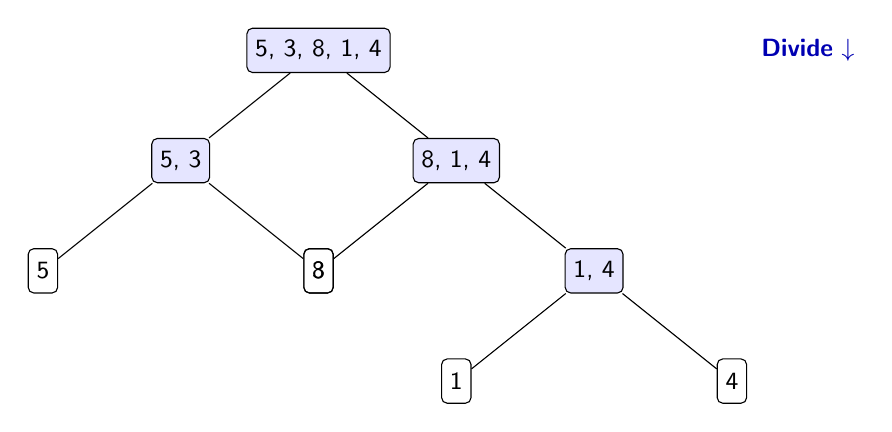
\begin{tikzpicture}[every node/.style={font=\small\sffamily}, >=Stealth,
  box/.style={draw, rounded corners=2pt, minimum height=1.6em, inner sep=3pt},
  level distance=1.4cm, sibling distance=3.5cm]
  \node[box, fill=blue!10] {5, 3, 8, 1, 4}
    child { node[box, fill=blue!10] {5, 3}
      child { node[box] {5} }
      child { node[box] {3} }
    }
    child { node[box, fill=blue!10] {8, 1, 4}
      child { node[box] {8} }
      child { node[box, fill=blue!10] {1, 4}
        child { node[box] {1} }
        child { node[box] {4} }
      }
    };
  \node at (5.5,-0.0) [anchor=west, text=blue!70!black] {\textbf{Divide} $\downarrow$};
\end{tikzpicture}
\end{center}
\vspace{-0.2cm}
\begin{center}
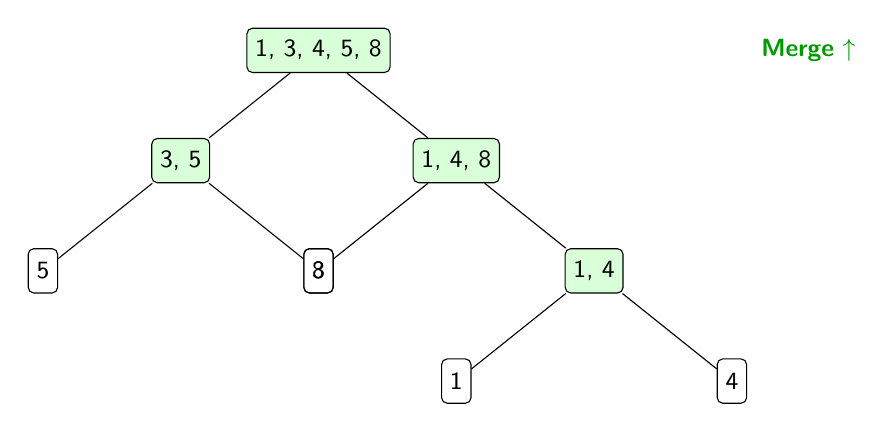
\begin{tikzpicture}[every node/.style={font=\small\sffamily}, >=Stealth,
  box/.style={draw, rounded corners=2pt, minimum height=1.6em, inner sep=3pt},
  level distance=1.4cm, sibling distance=3.5cm]
  \node[box, fill=green!15] {1, 3, 4, 5, 8}
    child { node[box, fill=green!15] {3, 5}
      child { node[box] {5} }
      child { node[box] {3} }
    }
    child { node[box, fill=green!15] {1, 4, 8}
      child { node[box] {8} }
      child { node[box, fill=green!15] {1, 4}
        child { node[box] {1} }
        child { node[box] {4} }
      }
    };
  \node at (5.5,-0.0) [anchor=west, text=green!60!black] {\textbf{Merge} $\uparrow$};
\end{tikzpicture}
\end{center}
\captionof{figure}{Merge Sort -- Chia (Divide) và Trộn (Merge) trên mảng $[5, 3, 8, 1, 4]$}\label{fig:merge-sort}

\begin{traceyourself}{Insertion Sort -- Trace mảng}
Cho mảng $A = [5, 3, 8, 1, 4]$. Tự trace Insertion Sort, điền mảng sau mỗi bước:

\begin{center}
\begin{tabular}{|c|c|l|}
\hline
\textbf{$j$} & \textbf{key} & \textbf{Mảng $A$ sau bước} \\
\hline
-- & -- & $[5, 3, 8, 1, 4]$ \\
\hline
2 & 3 & $[\underline{\hspace{4cm}}]$ \\
\hline
3 & 8 & $[\underline{\hspace{4cm}}]$ \\
\hline
4 & 1 & $[\underline{\hspace{4cm}}]$ \\
\hline
5 & 4 & $[\underline{\hspace{4cm}}]$ \\
\hline
\end{tabular}
\end{center}
\end{traceyourself}

\subsection{2.6 Quick Sort -- CLRS Ch.7}\label{quick-sort-clrs-ch.7}

\begin{tcolorbox}[colback=gray!8, colframe=gray!50, boxrule=0.5pt, arc=2pt,
  left=6pt, right=6pt, top=4pt, bottom=4pt,
  title={\small\textbf{Pseudocode 6: Quick Sort}}]
\begin{verbatim}
QuickSort(A, p, r):
    if p < r:
        q = Partition(A, p, r)
        QuickSort(A, p, q-1)
        QuickSort(A, q+1, r)

Partition(A, p, r):              // CLRS 7.1
    pivot = A[r]
    i = p - 1
    for j = p to r-1:
        if A[j] <= pivot:
            i = i + 1
            swap(A[i], A[j])
    swap(A[i+1], A[r])
    return i + 1
\end{verbatim}
\end{tcolorbox}

\begin{tcolorbox}[colback=yellow!5, colframe=orange!50, boxrule=0.5pt, arc=2pt, title={\small\textbf{Phân tích Complexity -- Quick Sort}}]
\begin{tabular}{|l|l|l|}
\hline
\textbf{Bước} & \textbf{Chi phí} & \textbf{Giải thích} \\
\hline
\textbf{Partition:} duyệt $n-1$ phần tử & $\Theta(n)$ & 1 vòng for \\
\hline
\textbf{Đệ quy 2 nửa} & $T(k) + T(n-k-1)$ & $k$ = vị trí pivot \\
\hline
\end{tabular}
\vspace{0.2cm}

\textbf{Best case} (pivot chia đều): $T(n)=2T(n/2)+\Theta(n)$ $\to$ $\Theta(n\lg n)$.\\
\textbf{Worst case} (pivot lệch cực): $T(n)=T(n-1)+\Theta(n)$ $\to$ $\Theta(n^2)$.\\
\textbf{Average case:} Mọi cách chia trung bình cho $\Theta(n\lg n)$.\\
\textbf{Space:} Stack đệ quy sâu $O(\lg n)$ avg, $O(n)$ worst. Không cần mảng phụ (in-place).
\end{tcolorbox}

\subsubsection{Ý tưởng}
Chọn một phần tử làm \textbf{pivot} (thường là phần tử cuối). Dùng \texttt{Partition} để chia mảng thành 2 phần: bên trái $\leq$ pivot, bên phải $>$ pivot. Pivot nằm đúng vị trí cuối cùng. Đệ quy sắp xếp 2 nửa. \textbf{Khác Merge Sort:} công việc nặng nằm ở bước \textit{chia} (Partition), còn merge thì miễn phí (đã in-place). Average $\Theta(n \lg n)$, worst $\Theta(n^2)$ khi pivot luôn lệch cực đoan.

\subsubsection{\texorpdfstring{Loop Invariant cho Partition (CLRS
\S 7.1):}{Loop Invariant cho Partition (CLRS 7.1):}}\label{loop-invariant-cho-partition-clrs-7.1}

Tại đầu mỗi lần lặp for:

\begin{enumerate}
\def\labelenumi{\arabic{enumi}.}
\tightlist
\item
  \(A[p..i]\): tất cả \(\leq\) pivot
\item
  \(A[i+1..j-1]\): tất cả \(>\) pivot
\item
  \(A[r] =\) pivot
\end{enumerate}

\subsubsection{Minh họa Animation}

\textbf{Bước 1 -- Partition toàn mảng:} $[5, 3, 8, 1, 4]$, Pivot = $A[5] = 4$, $i$ bắt đầu tại $0$.

\begin{sortanimation}
  \matrix (M) [matrix of nodes, nodes={normal}, column sep=-\pgflinewidth, row sep=0.7cm] {
    |[compare]| 5 & 3 & 8 & 1 & |[pivot]| 4 \\
    5 & |[compare]| 3 & 8 & 1 & |[pivot]| 4 \\
    |[sorted]| 3 & 5 & |[compare]| 8 & 1 & |[pivot]| 4 \\
    |[sorted]| 3 & |[compare]| 5 & 8 & |[compare]| 1 & |[pivot]| 4 \\
    |[sorted]| 3 & |[sorted]| 1 & |[compare]| 8 & 5 & |[pivot]| 4 \\
    |[sorted]| 3 & |[sorted]| 1 & |[pivot]| 4 & 5 & 8 \\
  };
  \node[right=0.5cm of M-1-5, anchor=west] {$j=1$: $5 > 4 \to$ Bỏ qua. $i=0$};

  \draw[<->, thick, blue!80!black, bend left=25] (M-2-1.south) to (M-2-2.south);
  \node[right=0.5cm of M-2-5, anchor=west] {$j=2$: $3 \leq 4 \to i=1$, Swap $A[1] \leftrightarrow A[2]$ (5 \& 3)};

  \node[right=0.5cm of M-3-5, anchor=west] {$j=3$: $8 > 4 \to$ Bỏ qua. $i=1$};

  \draw[<->, thick, blue!80!black, bend left=25] (M-4-2.south) to (M-4-4.south);
  \node[right=0.5cm of M-4-5, anchor=west] {$j=4$: $1 \leq 4 \to i=2$, Swap $A[2] \leftrightarrow A[4]$ (5 \& 1)};

  \draw[<->, thick, blue!80!black, bend left=25] (M-5-3.south) to (M-5-5.south);
  \node[right=0.5cm of M-5-5, anchor=west] {Hết vòng for. Swap $A[i{+}1] \leftrightarrow A[r]$ = $A[3] \leftrightarrow A[5]$ (8 \& 4)};

  \node[right=0.5cm of M-6-5, anchor=west] {Partition xong: $[3, 1, \boxed{4}, 5, 8]$. Pivot ở $q=3$.};
\end{sortanimation}

\textbf{Bước 2 -- Đệ quy trái} QuickSort($A, 1, 2$) trên $[3, 1]$: Pivot = $A[2] = 1$.

\begin{sortanimation}
  \matrix (M2) [matrix of nodes, nodes={normal}, column sep=-\pgflinewidth, row sep=0.7cm] {
    |[compare]| 3 & |[pivot]| 1 \\
    |[sorted]| 1 & 3 \\
  };
  \node[right=0.5cm of M2-1-2, anchor=west] {$j=1$: $3 > 1 \to$ Bỏ qua. $i=0$. Swap $A[1] \leftrightarrow A[2]$ (3 \& 1)};
  \node[right=0.5cm of M2-2-2, anchor=west] {Pivot 1 ở vị trí $q=1$. Mảng con: $[\boxed{1}, 3]$};
\end{sortanimation}

\textbf{Bước 3 -- Đệ quy phải} QuickSort($A, 4, 5$) trên $[5, 8]$: Pivot = $A[5] = 8$.

\begin{sortanimation}
  \matrix (M3) [matrix of nodes, nodes={normal}, column sep=-\pgflinewidth, row sep=0.7cm] {
    |[compare]| 5 & |[pivot]| 8 \\
    |[sorted]| 5 & |[sorted]| 8 \\
  };
  \node[right=0.5cm of M3-1-2, anchor=west] {$j=4$: $5 \leq 8 \to i=4$, Swap $A[4] \leftrightarrow A[4]$ (không đổi)};
  \node[right=0.5cm of M3-2-2, anchor=west] {Pivot 8 ở vị trí $q=5$. Mảng con: $[5, \boxed{8}]$ -- đã đúng};
\end{sortanimation}

\textbf{Kết quả cuối cùng:}
\begin{sortanimation}
  \matrix (MF) [matrix of nodes, nodes={sorted}, column sep=-\pgflinewidth] {
    1 & 3 & 4 & 5 & 8 \\
  };
  \node[right=0.5cm of MF-1-5, anchor=west] {Mảng đã được sắp xếp hoàn toàn! $[1, 3, 4, 5, 8]$};
\end{sortanimation}
\captionof{figure}{Quick Sort -- Toàn bộ quá trình sắp xếp trên mảng $[5, 3, 8, 1, 4]$}\label{fig:quick-sort}

\subsubsection{\texorpdfstring{Phân tích (CLRS \S 7.2,
7.4):}{Phân tích (CLRS 7.2, 7.4):}}\label{phuxe2n-tuxedch-clrs-7.2-7.4}

\begin{itemize}
\tightlist
\item
  \textbf{Worst case:} Partition luôn phân hoạch
  \((0, n-1) \to T(n) = T(n-1) + \Theta(n) = \Theta(n^2)\)
\item
  \textbf{Best case:} Partition phân hoạch đều
  \(\to T(n) = 2T(n/2) + \Theta(n) = \Theta(n \lg n)\)
\item
  \textbf{Average case (CLRS \S 7.4.2):} \(E[T(n)] = \Theta(n \lg n)\)
  -- chứng minh bằng indicator random variables
\end{itemize}

\subsubsection{\texorpdfstring{Randomized QuickSort (CLRS
\S 7.3):}{Randomized QuickSort (CLRS 7.3):}}\label{randomized-quicksort-clrs-7.3}

\begin{tcolorbox}[colback=gray!8, colframe=gray!50, boxrule=0.5pt, arc=2pt,
  left=6pt, right=6pt, top=4pt, bottom=4pt,
  title={\small\textbf{Pseudocode 7: Randomized Partition}}]
\begin{verbatim}
RandomizedPartition(A, p, r):
    i = Random(p, r)
    swap(A[i], A[r])
    return Partition(A, p, r)
\end{verbatim}
\end{tcolorbox}

Chọn pivot \textbf{ngẫu nhiên} \(\to\) Expected time =
\(\Theta(n \lg n)\), tránh worst case có hệ thống.

\subsubsection{Phân tích Complexity}
\begin{itemize}
\tightlist
\item \textbf{Best case:} Partition chia đều $\to$ $T(n) = 2T(n/2) + \Theta(n) = \Theta(n \lg n)$.
\item \textbf{Worst case:} Pivot luôn là min/max (mảng đã sắp + pivot cuối) $\to$ $T(n) = T(n{-}1) + \Theta(n) = \Theta(n^2)$.
\item \textbf{Average case:} Phân tích bằng indicator random variables: mọi cách chia đều cho $\Theta(n \lg n)$ trung bình.
\item \textbf{Space:} $O(\lg n)$ avg (stack đệ quy), $O(n)$ worst case. In-place (không cần mảng phụ). \textbf{Không stable}.
\end{itemize}

\checkpoint{Độ phức tạp worst case của Quick Sort là gì? Tại sao trong thực tế ta vẫn dùng Quick Sort thay vì Merge Sort? (Nêu 2 lý do.)}

\subsection{2.7 Heap Sort -- CLRS Ch.6}\label{heap-sort-clrs-ch.6}

\intuition{Heap Sort sử dụng cấu trúc \textbf{max-heap} (cây nhị phân hoàn chỉnh lưu trong mảng, gốc luôn lớn nhất). Bước 1: Xây heap $O(n)$. Bước 2: Lần lượt rút gốc (max) ra cuối mảng, rồi vá heap lại. Kết quả: worst case $\Theta(n \lg n)$, in-place, không cần bộ nhớ phụ.}

\subsubsection{Ý tưởng}

Heap Sort khai thác cấu trúc \textbf{heap} -- cây nhị phân hoàn chỉnh lưu ngay trong mảng -- để sắp xếp qua 2 bước:

\begin{enumerate}
\item \textbf{BuildMaxHeap} ($O(n)$): Biến mảng bất kỳ thành max-heap. Mảng $A$ được coi là cây nhị phân: nút $i$ có con trái = $2i$, con phải = $2i+1$. Gọi \texttt{MaxHeapify} từ $\lfloor n/2 \rfloor$ xuống $1$ để đảm bảo tính chất cha $\geq$ con tại mọi nút.
\item \textbf{Extract-Max lặp lại} ($O(n\lg n)$): Gốc $A[1]$ luôn là phần tử lớn nhất. Swap $A[1] \leftrightarrow A[n]$ (đưa max về cuối), giảm kích thước heap đi 1, rồi gọi \texttt{MaxHeapify(1)} để vá lại gốc. Lặp $n-1$ lần $\to$ mảng sắp tăng dần.
\end{enumerate}

\textbf{Tại sao hay?} Kết hợp ưu điểm: worst case $\Theta(n\lg n)$ như Merge Sort \textit{nhưng} in-place $O(1)$ space như Quick Sort.

\textbf{Tính chất Max-Heap:} $A[\lfloor i/2 \rfloor] \geq A[i]$ -- cha luôn $\geq$ con.

\textbf{Tính chất Min-Heap:} $A[\lfloor i/2 \rfloor] \leq A[i]$ -- cha luôn $\leq$ con. Gốc là phần tử \textbf{nhỏ nhất}.

\begin{tcolorbox}[colback=blue!3, colframe=blue!40, boxrule=0.5pt, arc=2pt, title={\small\textbf{So sánh Min-Heap vs Max-Heap}}]
\begin{tabular}{|l|l|l|}
\hline
 & \textbf{Max-Heap} & \textbf{Min-Heap} \\
\hline
\textbf{Tính chất} & Cha $\geq$ con & Cha $\leq$ con \\
\hline
\textbf{Gốc (root)} & Phần tử \textbf{lớn nhất} & Phần tử \textbf{nhỏ nhất} \\
\hline
\textbf{ExtractMax/Min} & $O(\lg n)$ -- rút max & $O(\lg n)$ -- rút min \\
\hline
\textbf{Insert} & $O(\lg n)$ & $O(\lg n)$ \\
\hline
\textbf{Build} & $O(n)$ & $O(n)$ \\
\hline
\textbf{Ứng dụng} & \textbf{Heap Sort} (rút max ra cuối) & \textbf{Dijkstra, Prim} (rút min priority) \\
\hline
\end{tabular}
\vspace{0.2cm}

\textbf{Tại sao Heap Sort dùng Max-Heap?} Vì ta muốn lần lượt rút phần tử \textit{lớn nhất} ra cuối mảng $\to$ mảng sắp tăng dần.\\
\textbf{Tại sao Dijkstra/Prim dùng Min-Heap?} Vì ta muốn \texttt{ExtractMin} -- luôn xử lý đỉnh có khoảng cách/key \textit{nhỏ nhất} trước (Greedy).
\end{tcolorbox}

\begin{tcolorbox}[colback=gray!8, colframe=gray!50, boxrule=0.5pt, arc=2pt,
  left=6pt, right=6pt, top=4pt, bottom=4pt,
  title={\small\textbf{Pseudocode 8: Heap Sort (MaxHeapify + BuildMaxHeap + HeapSort)}}]
\begin{verbatim}
MaxHeapify(A, i, n):             // CLRS 6.2
    l = 2*i;  r = 2*i + 1
    largest = i
    if l <= n and A[l] > A[largest]: largest = l
    if r <= n and A[r] > A[largest]: largest = r
    if largest != i:
        swap(A[i], A[largest])
        MaxHeapify(A, largest, n)

BuildMaxHeap(A, n):              // CLRS 6.3
    for i = floor(n/2) downto 1:
        MaxHeapify(A, i, n)

HeapSort(A, n):                  // CLRS 6.4
    BuildMaxHeap(A, n)
    for i = n downto 2:
        swap(A[1], A[i])
        MaxHeapify(A, 1, i-1)
\end{verbatim}
\end{tcolorbox}

\begin{tcolorbox}[colback=yellow!5, colframe=orange!50, boxrule=0.5pt, arc=2pt, title={\small\textbf{Phân tích Complexity -- Heap Sort}}]
\begin{tabular}{|l|l|l|}
\hline
\textbf{Thao tác} & \textbf{Chi phí} & \textbf{Giải thích} \\
\hline
\texttt{MaxHeapify(A, i)} & $O(\lg n)$ & đi xuống tối đa $\lg n$ tầng \\
\hline
\texttt{BuildMaxHeap(A)} & $O(n)$ & \textit{không phải} $O(n\lg n)$! \\
\hline
\quad (Lý do: $\sum_{h=0}^{\lg n}\lceil n/2^{h+1}\rceil \cdot O(h) = O(n)$) & & tổng telescoping \\
\hline
\texttt{HeapSort}: vòng for $n-1$ lần & $(n-1)\cdot O(\lg n)$ & swap gốc + MaxHeapify \\
\hline
\end{tabular}
\vspace{0.2cm}

\textbf{Time:} BuildMaxHeap $O(n)$ + HeapSort loop $O(n\lg n)$ $\to$ $\Theta(n\lg n)$ mọi trường hợp.\\
\textbf{Space:} $O(1)$ -- heap lưu ngay trong mảng $A$ (in-place), không cần mảng phụ.
\end{tcolorbox}

\subsubsection{Complexity}
BuildMaxHeap = $O(n)$. HeapSort = $\Theta(n \lg n)$ (worst, average, best). Space = $O(1)$ (in-place). Không stable.

\subsubsection{Loop Invariant}
\begin{itemize}
\tightlist
\item \textbf{Bất biến:} Tại đầu mỗi lần lặp \texttt{for i = n downto 2}: (1) $A[1..i]$ là max-heap, và (2) $A[i{+}1..n]$ chứa $n{-}i$ phần tử lớn nhất của mảng, đã sắp tăng dần.
\item \textbf{Init ($i=n$):} BuildMaxHeap vừa chạy xong $\to$ $A[1..n]$ là max-heap. $A[n{+}1..n]$ rỗng -- bất biến đúng.
\item \textbf{Maintenance:} $A[1]$ = max của heap $\to$ swap $A[1] \leftrightarrow A[i]$ $\to$ $A[i]$ đúng chỗ. Gọi MaxHeapify$(A, 1, i{-}1)$ để sửa heap. Bất biến đúng cho $i{-}1$.
\item \textbf{Termination ($i=1$):} $A[2..n]$ chứa $n{-}1$ phần tử lớn nhất, sắp. $A[1]$ là nhỏ nhất $\to$ mảng sắp. $\square$
\end{itemize}

\subsubsection{Minh họa Animation}

\textbf{Cây nhị phân (Binary Tree) biểu diễn Heap:}

Mảng $A = [5, 3, 8, 1, 4]$ được lưu trong heap theo quy tắc: nút $i$ có con trái = $2i$, con phải = $2i+1$.

\begin{center}
% ===== ROW 1: Before BuildMaxHeap (3 columns) =====
\begin{minipage}[t]{0.31\textwidth}
\centering
{\small\textbf{Ví dụ 1:} $[5,3,8,1,4]$}
\vspace{0.15cm}

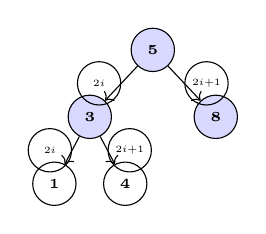
\begin{tikzpicture}[
  level distance=0.85cm,
  level 1/.style={sibling distance=1.6cm},
  level 2/.style={sibling distance=0.9cm},
  every node/.style={circle, draw, minimum size=5.5mm, font=\tiny\bfseries, inner sep=0pt},
  edge from parent/.style={draw, ->, thin}
]
\node[fill=blue!15] {5}
  child { node[fill=blue!15] {3}
    child { node {1} edge from parent node[left, font=\tiny\itshape] {\scalebox{0.7}{$2i$}} }
    child { node {4} edge from parent node[right, font=\tiny\itshape] {\scalebox{0.7}{$2i{+}1$}} }
    edge from parent node[left, font=\tiny\itshape] {\scalebox{0.7}{$2i$}}
  }
  child { node[fill=blue!15] {8}
    edge from parent node[right, font=\tiny\itshape] {\scalebox{0.7}{$2i{+}1$}}
  };
\end{tikzpicture}
\end{minipage}%
\hfill
\begin{minipage}[t]{0.31\textwidth}
\centering
{\small\textbf{Ví dụ 2:} $[5,3,8,1,4,6]$}
\vspace{0.15cm}

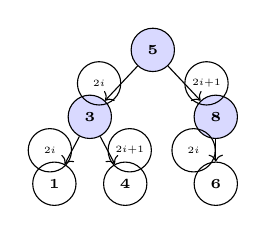
\begin{tikzpicture}[
  level distance=0.85cm,
  level 1/.style={sibling distance=1.6cm},
  level 2/.style={sibling distance=0.9cm},
  every node/.style={circle, draw, minimum size=5.5mm, font=\tiny\bfseries, inner sep=0pt},
  edge from parent/.style={draw, ->, thin}
]
\node[fill=blue!15] {5}
  child { node[fill=blue!15] {3}
    child { node {1} edge from parent node[left, font=\tiny\itshape] {\scalebox{0.7}{$2i$}} }
    child { node {4} edge from parent node[right, font=\tiny\itshape] {\scalebox{0.7}{$2i{+}1$}} }
    edge from parent node[left, font=\tiny\itshape] {\scalebox{0.7}{$2i$}}
  }
  child { node[fill=blue!15] {8}
    child { node {6} edge from parent node[left, font=\tiny\itshape] {\scalebox{0.7}{$2i$}} }
    edge from parent node[right, font=\tiny\itshape] {\scalebox{0.7}{$2i{+}1$}}
  };
\end{tikzpicture}
\end{minipage}%
\hfill
\begin{minipage}[t]{0.31\textwidth}
\centering
{\small\textbf{Ví dụ 3:} $[5,3,8,1,4,6,2]$}
\vspace{0.15cm}

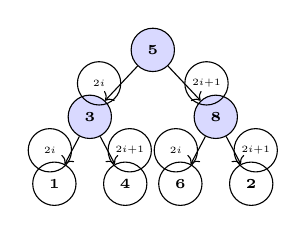
\begin{tikzpicture}[
  level distance=0.85cm,
  level 1/.style={sibling distance=1.6cm},
  level 2/.style={sibling distance=0.9cm},
  every node/.style={circle, draw, minimum size=5.5mm, font=\tiny\bfseries, inner sep=0pt},
  edge from parent/.style={draw, ->, thin}
]
\node[fill=blue!15] {5}
  child { node[fill=blue!15] {3}
    child { node {1} edge from parent node[left, font=\tiny\itshape] {\scalebox{0.7}{$2i$}} }
    child { node {4} edge from parent node[right, font=\tiny\itshape] {\scalebox{0.7}{$2i{+}1$}} }
    edge from parent node[left, font=\tiny\itshape] {\scalebox{0.7}{$2i$}}
  }
  child { node[fill=blue!15] {8}
    child { node {6} edge from parent node[left, font=\tiny\itshape] {\scalebox{0.7}{$2i$}} }
    child { node {2} edge from parent node[right, font=\tiny\itshape] {\scalebox{0.7}{$2i{+}1$}} }
    edge from parent node[right, font=\tiny\itshape] {\scalebox{0.7}{$2i{+}1$}}
  };
\end{tikzpicture}
\end{minipage}

\vspace{0.25cm}
$\Big\downarrow$ \textbf{BuildMaxHeap} (MaxHeapify từ $i = \lfloor n/2 \rfloor$ xuống $1$) $\Big\downarrow$
\vspace{0.25cm}

% ===== ROW 2: After BuildMaxHeap (3 columns) =====
\begin{minipage}[t]{0.31\textwidth}
\centering
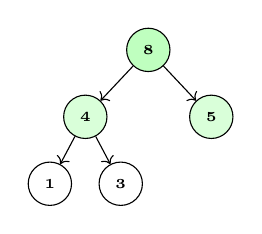
\begin{tikzpicture}[
  level distance=0.85cm,
  level 1/.style={sibling distance=1.6cm},
  level 2/.style={sibling distance=0.9cm},
  every node/.style={circle, draw, minimum size=5.5mm, font=\tiny\bfseries, inner sep=0pt},
  edge from parent/.style={draw, ->, thin}
]
\node[fill=green!25] {8}
  child { node[fill=green!15] {4}
    child { node {1} }
    child { node {3} }
  }
  child { node[fill=green!15] {5} };
\end{tikzpicture}

{\tiny $[\mathbf{8},4,5,1,3]$\\$8{\geq}4$\checkmark\ $8{\geq}5$\checkmark\ $4{\geq}1$\checkmark\ $4{\geq}3$\checkmark}
\end{minipage}%
\hfill
\begin{minipage}[t]{0.31\textwidth}
\centering
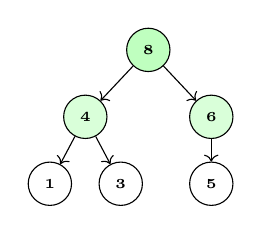
\begin{tikzpicture}[
  level distance=0.85cm,
  level 1/.style={sibling distance=1.6cm},
  level 2/.style={sibling distance=0.9cm},
  every node/.style={circle, draw, minimum size=5.5mm, font=\tiny\bfseries, inner sep=0pt},
  edge from parent/.style={draw, ->, thin}
]
\node[fill=green!25] {8}
  child { node[fill=green!15] {4}
    child { node {1} }
    child { node {3} }
  }
  child { node[fill=green!15] {6}
    child { node {5} }
  };
\end{tikzpicture}

{\tiny $[\mathbf{8},4,6,1,3,5]$\\$8{\geq}4$\checkmark\ $8{\geq}6$\checkmark\ $4{\geq}1$\checkmark\ $4{\geq}3$\checkmark\ $6{\geq}5$\checkmark}
\end{minipage}%
\hfill
\begin{minipage}[t]{0.31\textwidth}
\centering
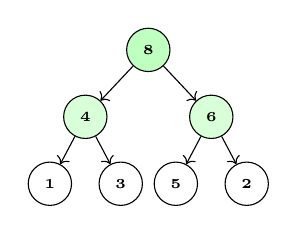
\begin{tikzpicture}[
  level distance=0.85cm,
  level 1/.style={sibling distance=1.6cm},
  level 2/.style={sibling distance=0.9cm},
  every node/.style={circle, draw, minimum size=5.5mm, font=\tiny\bfseries, inner sep=0pt},
  edge from parent/.style={draw, ->, thin}
]
\node[fill=green!25] {8}
  child { node[fill=green!15] {4}
    child { node {1} }
    child { node {3} }
  }
  child { node[fill=green!15] {6}
    child { node {5} }
    child { node {2} }
  };
\end{tikzpicture}

{\tiny $[\mathbf{8},4,6,1,3,5,2]$\\$8{\geq}4$\checkmark\ $8{\geq}6$\checkmark\ $4{\geq}1$\checkmark\ $4{\geq}3$\checkmark\ $6{\geq}5$\checkmark\ $6{\geq}2$\checkmark}
\end{minipage}

\vspace{0.25cm}
$\Big\downarrow$ \textbf{Extract-Max:} Swap $A[1] \leftrightarrow A[n]$, giảm heap, MaxHeapify$(1)$ $\Big\downarrow$
\vspace{0.25cm}

% ===== ROW 3: After first Extract-Max (3 columns) =====
\begin{minipage}[t]{0.31\textwidth}
\centering
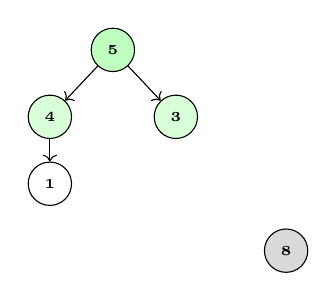
\begin{tikzpicture}[
  level distance=0.85cm,
  level 1/.style={sibling distance=1.6cm},
  level 2/.style={sibling distance=0.9cm},
  every node/.style={circle, draw, minimum size=5.5mm, font=\tiny\bfseries, inner sep=0pt},
  edge from parent/.style={draw, ->, thin}
]
\node[fill=green!25] {5}
  child { node[fill=green!15] {4}
    child { node {1} }
  }
  child { node[fill=green!15] {3} };
\node[fill=gray!30, circle, draw, minimum size=5.5mm, font=\tiny\bfseries, inner sep=0pt] at (2.2, -2.55) {8};
\end{tikzpicture}

{\tiny Swap $8 \leftrightarrow 3$, Heapify\\$[\mathbf{5},4,3,1\mid\boxed{8}]$}
\end{minipage}%
\hfill
\begin{minipage}[t]{0.31\textwidth}
\centering
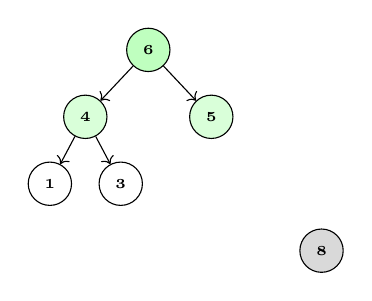
\begin{tikzpicture}[
  level distance=0.85cm,
  level 1/.style={sibling distance=1.6cm},
  level 2/.style={sibling distance=0.9cm},
  every node/.style={circle, draw, minimum size=5.5mm, font=\tiny\bfseries, inner sep=0pt},
  edge from parent/.style={draw, ->, thin}
]
\node[fill=green!25] {6}
  child { node[fill=green!15] {4}
    child { node {1} }
    child { node {3} }
  }
  child { node[fill=green!15] {5} };
\node[fill=gray!30, circle, draw, minimum size=5.5mm, font=\tiny\bfseries, inner sep=0pt] at (2.2, -2.55) {8};
\end{tikzpicture}

{\tiny Swap $8 \leftrightarrow 5$, Heapify\\$[\mathbf{6},4,5,1,3\mid\boxed{8}]$}
\end{minipage}%
\hfill
\begin{minipage}[t]{0.31\textwidth}
\centering
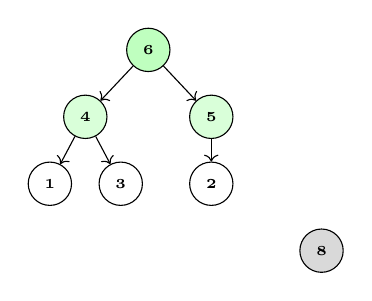
\begin{tikzpicture}[
  level distance=0.85cm,
  level 1/.style={sibling distance=1.6cm},
  level 2/.style={sibling distance=0.9cm},
  every node/.style={circle, draw, minimum size=5.5mm, font=\tiny\bfseries, inner sep=0pt},
  edge from parent/.style={draw, ->, thin}
]
\node[fill=green!25] {6}
  child { node[fill=green!15] {4}
    child { node {1} }
    child { node {3} }
  }
  child { node[fill=green!15] {5}
    child { node {2} }
  };
\node[fill=gray!30, circle, draw, minimum size=5.5mm, font=\tiny\bfseries, inner sep=0pt] at (2.2, -2.55) {8};
\end{tikzpicture}

{\tiny Swap $8 \leftrightarrow 2$, Heapify\\$[\mathbf{6},4,5,1,3,2\mid\boxed{8}]$}
\end{minipage}

\vspace{0.25cm}
$\Big\downarrow$ \textbf{Extract-Max lần 2:} Swap gốc $\leftrightarrow$ cuối heap, MaxHeapify$(1)$ $\Big\downarrow$
\vspace{0.25cm}

% ===== ROW 4: After second Extract-Max (3 columns) =====
\begin{minipage}[t]{0.31\textwidth}
\centering
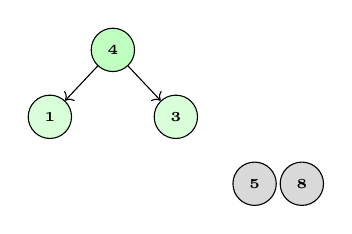
\begin{tikzpicture}[
  level distance=0.85cm,
  level 1/.style={sibling distance=1.6cm},
  level 2/.style={sibling distance=0.9cm},
  every node/.style={circle, draw, minimum size=5.5mm, font=\tiny\bfseries, inner sep=0pt},
  edge from parent/.style={draw, ->, thin}
]
\node[fill=green!25] {4}
  child { node[fill=green!15] {1} }
  child { node[fill=green!15] {3} };
\node[fill=gray!30, circle, draw, minimum size=5.5mm, font=\tiny\bfseries, inner sep=0pt] at (1.8, -1.7) {5};
\node[fill=gray!30, circle, draw, minimum size=5.5mm, font=\tiny\bfseries, inner sep=0pt] at (2.4, -1.7) {8};
\end{tikzpicture}

{\tiny Swap $5 \leftrightarrow 1$, Heapify\\$[\mathbf{4},1,3\mid\boxed{5},\boxed{8}]$}
\end{minipage}%
\hfill
\begin{minipage}[t]{0.31\textwidth}
\centering
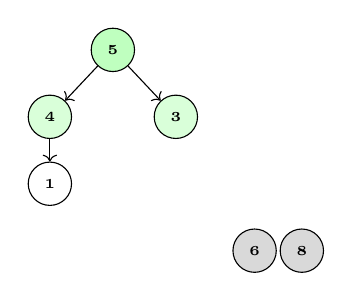
\begin{tikzpicture}[
  level distance=0.85cm,
  level 1/.style={sibling distance=1.6cm},
  level 2/.style={sibling distance=0.9cm},
  every node/.style={circle, draw, minimum size=5.5mm, font=\tiny\bfseries, inner sep=0pt},
  edge from parent/.style={draw, ->, thin}
]
\node[fill=green!25] {5}
  child { node[fill=green!15] {4}
    child { node {1} }
  }
  child { node[fill=green!15] {3} };
\node[fill=gray!30, circle, draw, minimum size=5.5mm, font=\tiny\bfseries, inner sep=0pt] at (1.8, -2.55) {6};
\node[fill=gray!30, circle, draw, minimum size=5.5mm, font=\tiny\bfseries, inner sep=0pt] at (2.4, -2.55) {8};
\end{tikzpicture}

{\tiny Swap $6 \leftrightarrow 3$, Heapify\\$[\mathbf{5},4,3,1\mid\boxed{6},\boxed{8}]$}
\end{minipage}%
\hfill
\begin{minipage}[t]{0.31\textwidth}
\centering
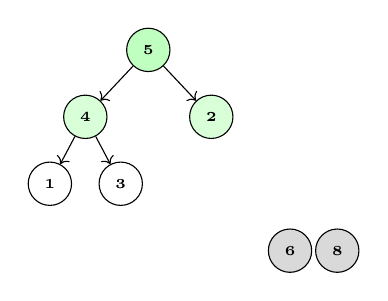
\begin{tikzpicture}[
  level distance=0.85cm,
  level 1/.style={sibling distance=1.6cm},
  level 2/.style={sibling distance=0.9cm},
  every node/.style={circle, draw, minimum size=5.5mm, font=\tiny\bfseries, inner sep=0pt},
  edge from parent/.style={draw, ->, thin}
]
\node[fill=green!25] {5}
  child { node[fill=green!15] {4}
    child { node {1} }
    child { node {3} }
  }
  child { node[fill=green!15] {2} };
\node[fill=gray!30, circle, draw, minimum size=5.5mm, font=\tiny\bfseries, inner sep=0pt] at (1.8, -2.55) {6};
\node[fill=gray!30, circle, draw, minimum size=5.5mm, font=\tiny\bfseries, inner sep=0pt] at (2.4, -2.55) {8};
\end{tikzpicture}

{\tiny Swap $6 \leftrightarrow 2$, Heapify\\$[\mathbf{5},4,2,1,3\mid\boxed{6},\boxed{8}]$}
\end{minipage}
\end{center}

\textbf{Bước 1 -- BuildMaxHeap:} $[5, 3, 8, 1, 4]$

\begin{sortanimation}
  \matrix (H1) [matrix of nodes, nodes={normal}, column sep=-\pgflinewidth, row sep=0.6cm] {
    5 & |[compare]| 3 & 8 & 1 & 4 \\
    5 & |[sorted]| 4 & 8 & 1 & 3 \\
    |[compare]| 5 & 4 & |[compare]| 8 & 1 & 3 \\
    |[pivot]| 8 & 4 & 5 & 1 & 3 \\
  };
  \draw[<->, thick, blue!80!black, bend left=25] (H1-1-2.south) to (H1-1-5.south);
  \node[right=0.5cm of H1-1-5, anchor=west] {$i=2$: $A[2]{=}3$, con $A[5]{=}4 > 3 \to$ Swap};
  \node[right=0.5cm of H1-2-5, anchor=west] {Kết quả: $[5, 4, 8, 1, 3]$};
  \draw[<->, thick, blue!80!black, bend left=25] (H1-3-1.south) to (H1-3-3.south);
  \node[right=0.5cm of H1-3-5, anchor=west] {$i=1$: $A[1]{=}5$, con $A[3]{=}8 > 5 \to$ Swap};
  \node[right=0.5cm of H1-4-5, anchor=west] {Max-Heap: $[\mathbf{8}, 4, 5, 1, 3]$};
\end{sortanimation}

\textbf{Bước 2 -- Extract-Max lần lượt:}

\begin{sortanimation}
  \matrix (H2) [matrix of nodes, nodes={normal}, column sep=-\pgflinewidth, row sep=0.6cm] {
    |[pivot]| 8 & 4 & 5 & 1 & 3 \\
    |[compare]| 3 & 4 & 5 & 1 & |[sorted]| 8 \\
    |[pivot]| 5 & 4 & 3 & 1 & |[sorted]| 8 \\
    |[compare]| 1 & 4 & 3 & |[sorted]| 5 & |[sorted]| 8 \\
    |[pivot]| 4 & 1 & 3 & |[sorted]| 5 & |[sorted]| 8 \\
    |[compare]| 3 & 1 & |[sorted]| 4 & |[sorted]| 5 & |[sorted]| 8 \\
    |[pivot]| 3 & 1 & |[sorted]| 4 & |[sorted]| 5 & |[sorted]| 8 \\
    |[sorted]| 1 & |[sorted]| 3 & |[sorted]| 4 & |[sorted]| 5 & |[sorted]| 8 \\
  };
  \node[right=0.5cm of H2-1-5, anchor=west] {Heap: $[8, 4, 5, 1, 3]$};
  \draw[<->, thick, blue!80!black, bend left=20] (H2-2-1.south) to (H2-2-5.south);
  \node[right=0.5cm of H2-2-5, anchor=west] {Swap $A[1] \leftrightarrow A[5]$. Heapify $\to$};
  \node[right=0.5cm of H2-3-5, anchor=west] {$[\mathbf{5}, 4, 3, 1 \mid 8]$};
  \draw[<->, thick, blue!80!black, bend left=20] (H2-4-1.south) to (H2-4-4.south);
  \node[right=0.5cm of H2-4-5, anchor=west] {Swap $A[1] \leftrightarrow A[4]$. Heapify $\to$};
  \node[right=0.5cm of H2-5-5, anchor=west] {$[\mathbf{4}, 1, 3 \mid 5, 8]$};
  \draw[<->, thick, blue!80!black, bend left=20] (H2-6-1.south) to (H2-6-3.south);
  \node[right=0.5cm of H2-6-5, anchor=west] {Swap $A[1] \leftrightarrow A[3]$. Heapify $\to$};
  \node[right=0.5cm of H2-7-5, anchor=west] {$[\mathbf{3}, 1 \mid 4, 5, 8]$. Swap $A[1] \leftrightarrow A[2]$:};
  \node[right=0.5cm of H2-8-5, anchor=west] {Mảng đã sắp xếp: $[1, 3, 4, 5, 8]$};
\end{sortanimation}
\captionof{figure}{Heap Sort -- Toàn bộ quá trình sắp xếp trên mảng $[5, 3, 8, 1, 4]$}\label{fig:heap-sort}

\subsection{\texorpdfstring{Cận dưới cho sắp xếp so sánh -- CLRS
\S 8.1}{Cận dưới cho sắp xếp so sánh -- CLRS 8.1}}\label{cux1eadn-dux1b0ux1edbi-cho-sux1eafp-xux1ebfp-so-suxe1nh-clrs-8.1}

\begin{quote}
\textbf{Định lý (CLRS Theorem 8.1):} Mọi thuật toán sắp xếp dựa trên so
sánh cần \(\Omega(n \lg n)\) phép so sánh trong worst case.
\end{quote}

\textbf{Chứng minh:} Cây quyết định (decision tree) có \(n!\) lá \(\to\)
chiều cao \(\geq \lg(n!) = \Omega(n \lg n)\).

\(\to\) \textbf{Merge Sort và Quick Sort (average) đều TỐI ƯU} cho
comparison sorting!

\subsection{2.8 Counting Sort -- CLRS Ch.8}\label{counting-sort}

\subsubsection{Ý tưởng}
Thay vì so sánh, ta \textbf{đếm} số lần xuất hiện của mỗi giá trị. Tạo mảng đếm $C[0..k]$, với $C[x]$ = số phần tử $= x$. Cộng dồn $C$ để biết vị trí cuối cùng của mỗi giá trị trong output. Duyệt ngược mảng gốc, đặt từng phần tử vào đúng vị trí $\to$ \textbf{stable}, $O(n+k)$. Chỉ dùng khi biết phạm vi giá trị $k$ và $k$ không quá lớn.

\begin{tcolorbox}[colback=gray!8, colframe=gray!50, boxrule=0.5pt, arc=2pt,
  left=6pt, right=6pt, top=4pt, bottom=4pt,
  title={\small\textbf{Pseudocode 9: Counting Sort (CLRS 8.2)}}]
\begin{verbatim}
CountingSort(A, B, n, k):
    // A: input, B: output, k: max value
    let C[0..k] = all zeros
    for j = 1 to n:
        C[A[j]] = C[A[j]] + 1      // dem tan suat
    for i = 1 to k:
        C[i] = C[i] + C[i-1]       // cong don -> vi tri
    for j = n downto 1:             // duyet NGUOC -> stable
        B[C[A[j]]] = A[j]
        C[A[j]] = C[A[j]] - 1
\end{verbatim}
\end{tcolorbox}

\begin{tcolorbox}[colback=yellow!5, colframe=orange!50, boxrule=0.5pt, arc=2pt, title={\small\textbf{Phân tích Complexity -- Counting Sort}}]
\begin{tabular}{|l|l|l|}
\hline
\textbf{Dòng code} & \textbf{Số lần chạy} & \textbf{Chi phí} \\
\hline
\texttt{let C[0..k] = all zeros} & $k+1$ & khởi tạo mảng đếm \\
\hline
\texttt{for j = 1 to n: C[A[j]]++} & $n$ & đếm tần suất \\
\hline
\texttt{for i = 1 to k: C[i] += C[i-1]} & $k$ & cộng dồn \\
\hline
\texttt{for j = n downto 1: B[C[A[j]]]=A[j]} & $n$ & đặt vào output \\
\hline
\end{tabular}
\vspace{0.2cm}

\textbf{Time:} $\Theta(n+k)$ -- 2 vòng $\Theta(n)$ + 1 vòng $\Theta(k)$. \textit{Tuyến tính} khi $k=O(n)$.\\
\textbf{Space:} Mảng $C[0..k]$: $\Theta(k)$ + mảng output $B[1..n]$: $\Theta(n)$ $\to$ $\Theta(n+k)$. \textit{Không} in-place.
\end{tcolorbox}

\subsubsection{Complexity}
$\Theta(n + k)$ time, $\Theta(n + k)$ space. Stable. \textbf{Không dựa trên so sánh} -- vì vậy không bị ràng buộc bởi cận dưới $\Omega(n \lg n)$.

\whyprompt{Tại sao \textbf{Counting Sort} không vi phạm cận dưới $\Omega(n \lg n)$, dù nó chạy $O(n+k)$? Gợi ý: xem lại điều kiện ``sắp xếp dựa trên so sánh'' trong Theorem 8.1 (CLRS).}

\begin{center}\rule{0.5\linewidth}{0.5pt}\end{center}

\section{Chương 3: Định lý Thợ và Giải đệ quy -- Master Theorem \& Solving Recurrences (CLRS Ch.4)}\label{chux1b0ux1a1ng-3-master-theorem-giux1ea3i-ux111ux1ec7-quy-clrs-ch.4}

\intuition{Hầu hết thuật toán Divide \& Conquer đều có công thức đệ quy dạng $T(n) = aT(n/b) + f(n)$. Master Theorem là \textbf{công thức cookbook} giải ngay đa số trường hợp. Nếu không áp dụng được, dùng Recursion Tree để vẽ trực quan tổng chi phí theo từng tầng đệ quy.}

\pitfall{(1) Master Theorem không áp dụng được khi $b < 1$ hoặc $a < 1$, hoặc khi $f(n)$ không đơn điệu. (2) Case 3 đòi hỏi điều kiện \textbf{regularity} $af(n/b) \leq cf(n)$ -- nhiều người quên kiểm tra. (3) $T(n) = 2T(n/2) + n\lg n$ là Case 2 (không phải Case 3) vì $f(n) = n\lg n = \Theta(n^{\log_2 2} \cdot \lg n)$.}


\subsection{Ý tưởng Chia để trị (Divide \& Conquer)}\label{y-tuong-dc}

Divide \& Conquer là mô hình thiết kế thuật toán gồm \textbf{3 bước}:

\begin{enumerate}
\item \textbf{Divide (Chia):} Chia bài toán kích thước $n$ thành $a$ bài toán con kích thước $n/b$.
\item \textbf{Conquer (Trị):} Giải đệ quy từng bài toán con. Nếu bài toán con đủ nhỏ, giải trực tiếp (base case).
\item \textbf{Combine (Kết hợp):} Gộp nghiệm các bài toán con thành nghiệm bài toán gốc.
\end{enumerate}

\textbf{Công thức đệ quy tổng quát:}
\[T(n) = aT(n/b) + f(n)\]
trong đó $a$ = số bài toán con, $n/b$ = kích thước mỗi bài con, $f(n)$ = chi phí chia + gộp.

\textbf{Ví dụ điển hình:}
\begin{itemize}
\item \textbf{Merge Sort:} $a=2, b=2, f(n)=\Theta(n)$ (chia giữa, merge $\Theta(n)$) $\to T(n)=\Theta(n\lg n)$.
\item \textbf{Quick Sort:} $a=2, b$ phụ thuộc pivot, $f(n)=\Theta(n)$ (Partition).
\item \textbf{Binary Search:} $a=1, b=2, f(n)=\Theta(1)$ $\to T(n)=\Theta(\lg n)$.
\end{itemize}

\subsection{\texorpdfstring{Ba phương pháp giải đệ quy (CLRS
\S 4.3-4.5)}{Ba phương pháp giải đệ quy (CLRS 4.3-4.5)}}\label{ba-phux1b0ux1a1ng-phuxe1p-giux1ea3i-ux111ux1ec7-quy-clrs-4.3-4.5}

\subsubsection{\texorpdfstring{Phương pháp 1: Substitution Method (Thay
thế) -- CLRS
\S 4.3}{Phương pháp 1: Substitution Method (Thay thế) -- CLRS 4.3}}\label{phux1b0ux1a1ng-phuxe1p-1-substitution-method-thay-thux1ebf-clrs-4.3}

\begin{enumerate}
\def\labelenumi{\arabic{enumi}.}
\tightlist
\item
  \textbf{Đoán} dạng nghiệm
\item
  \textbf{Chứng minh} bằng quy nạp toán học
\end{enumerate}

\textbf{Ví dụ:} \(T(n) = 2T(\lfloor n/2 \rfloor) + n\), đoán
\(T(n) = O(n \lg n)\).

\begin{itemize}
\tightlist
\item
  Giả sử
  \(T(\lfloor n/2 \rfloor) \leq c \cdot \lfloor n/2 \rfloor \cdot \lg(\lfloor n/2 \rfloor)\)
\item
  \(T(n) \leq 2 c (n/2) \lg(n/2) + n = cn \lg n - cn \lg 2 + n = cn \lg n - cn + n\)
\item
  \(\leq cn \lg n\) khi \(c \geq 1\) (OK)
\end{itemize}

\subsubsection{\texorpdfstring{Phương pháp 2: Recursion Tree (Cây đệ
quy) -- CLRS
\S 4.4}{Phương pháp 2: Recursion Tree (Cây đệ quy) -- CLRS 4.4}}\label{phux1b0ux1a1ng-phuxe1p-2-recursion-tree-cuxe2y-ux111ux1ec7-quy-clrs-4.4}

Vẽ cây, mỗi nút là chi phí tại mức đệ quy đó.

\textbf{Ví dụ:} \(T(n) = 3T(n/4) + cn^2\)

\begin{tcolorbox}[colback=gray!8, colframe=gray!50, boxrule=0.5pt, arc=2pt,
  left=6pt, right=6pt, top=4pt, bottom=4pt,
  title={\small\textbf{Pseudocode 9: Cây đệ quy (Recursion Tree)}}]
\begin{verbatim}
Muc 0:  cn^2                              -> cn^2
Muc 1:  3 * c(n/4)^2                      -> (3/16) cn^2
Muc 2:  9 * c(n/16)^2                     -> (3/16)^2 cn^2
...
Muc i:  3^i * c(n/4^i)^2                  -> (3/16)^i cn^2
...
Muc log_4(n): 3^(log_4 n) nut, Theta(1)   -> Theta(n^(log_4 3))

Tong = cn^2 * Sum (3/16)^i (i=0..inf) = cn^2 * 16/13 = O(n^2)
\end{verbatim}
\end{tcolorbox}

\subsubsection{\texorpdfstring{Phương pháp 3: Master Theorem -- CLRS
\S 4.5}{Phương pháp 3: Master Theorem -- CLRS 4.5}}\label{phux1b0ux1a1ng-phuxe1p-3-master-theorem-clrs-4.5}

\textbf{Cho \(T(n) = aT(n/b) + f(n)\),} \(a \geq 1, b > 1\):

{\def\LTcaptype{none} % do not increment counter
\begin{longtable}[]{@{}
  >{\raggedright\arraybackslash}p{(\linewidth - 4\tabcolsep) * \real{0.3333}}
  >{\raggedright\arraybackslash}p{(\linewidth - 4\tabcolsep) * \real{0.3333}}
  >{\raggedright\arraybackslash}p{(\linewidth - 4\tabcolsep) * \real{0.3333}}@{}}
\toprule\noalign{}
\begin{minipage}[b]{\linewidth}\raggedright
Case
\end{minipage} & \begin{minipage}[b]{\linewidth}\raggedright
Điều kiện
\end{minipage} & \begin{minipage}[b]{\linewidth}\raggedright
Kết quả
\end{minipage} \\
\midrule\noalign{}
\endhead
\bottomrule\noalign{}
\endlastfoot
\textbf{1} & \(f(n) = O(n^{\log_b a - \varepsilon})\) với
\(\varepsilon > 0\) & \(T(n) = \Theta(n^{\log_b a})\) \\
\textbf{2} & \(f(n) = \Theta(n^{\log_b a} \cdot \lg^k n)\) &
\(T(n) = \Theta(n^{\log_b a} \cdot \lg^{k+1} n)\) \\
\textbf{3} & \(f(n) = \Omega(n^{\log_b a + \varepsilon})\) với
\(\varepsilon > 0\) \textbf{VÀ} \(a f(n/b) \leq c f(n)\) với \(c < 1\) &
\(T(n) = \Theta(f(n))\) \\
\end{longtable}
}
\captionof{table}{Master Theorem -- Ba trường hợp}\label{tab:master-theorem}

\subsubsection{Ví dụ áp dụng:}\label{vuxed-dux1ee5-uxe1p-dux1ee5ng}

{\def\LTcaptype{none} % do not increment counter
\begin{longtable}[]{@{}
  >{\raggedright\arraybackslash}p{(\linewidth - 12\tabcolsep) * \real{0.1429}}
  >{\raggedright\arraybackslash}p{(\linewidth - 12\tabcolsep) * \real{0.1429}}
  >{\raggedright\arraybackslash}p{(\linewidth - 12\tabcolsep) * \real{0.1429}}
  >{\raggedright\arraybackslash}p{(\linewidth - 12\tabcolsep) * \real{0.1429}}
  >{\raggedright\arraybackslash}p{(\linewidth - 12\tabcolsep) * \real{0.1429}}
  >{\raggedright\arraybackslash}p{(\linewidth - 12\tabcolsep) * \real{0.1429}}
  >{\raggedright\arraybackslash}p{(\linewidth - 12\tabcolsep) * \real{0.1429}}@{}}
\toprule\noalign{}
\begin{minipage}[b]{\linewidth}\raggedright
Đệ quy
\end{minipage} & \begin{minipage}[b]{\linewidth}\raggedright
a
\end{minipage} & \begin{minipage}[b]{\linewidth}\raggedright
b
\end{minipage} & \begin{minipage}[b]{\linewidth}\raggedright
\(\log_b a\)
\end{minipage} & \begin{minipage}[b]{\linewidth}\raggedright
\(f(n)\)
\end{minipage} & \begin{minipage}[b]{\linewidth}\raggedright
Case
\end{minipage} & \begin{minipage}[b]{\linewidth}\raggedright
Kết quả
\end{minipage} \\
\midrule\noalign{}
\endhead
\bottomrule\noalign{}
\endlastfoot
\(T(n) = 2T(n/2) + n\) & 2 & 2 & 1 & \(n\) & 2 (\(k=0\)) &
\(\Theta(n \lg n)\) \\
\(T(n) = T(n/2) + 1\) & 1 & 2 & 0 & 1 & 2 (\(k=0\)) &
\(\Theta(\lg n)\) \\
\(T(n) = 7T(n/2) + n^2\) & 7 & 2 & 2.807 & \(n^2\) & 1
(\(\varepsilon \approx 0.8\)) & \(\Theta(n^{2.807})\) \\
\(T(n) = 9T(n/3) + n\) & 9 & 3 & 2 & \(n\) & 1 (\(\varepsilon = 1\)) &
\(\Theta(n^2)\) \\
\(T(n) = T(2n/3) + 1\) & 1 & 3/2 & 0 & 1 & 2 (\(k=0\)) &
\(\Theta(\lg n)\) \\
\end{longtable}
}
\captionof{table}{Ví dụ áp dụng Master Theorem}\label{tab:master-examples}

\begin{center}\rule{0.5\linewidth}{0.5pt}\end{center}

\section{Chương 4: Lý thuyết Đồ thị -- Graph Theory (CLRS Ch.22)}\label{chux1b0ux1a1ng-4-luxfd-thuyux1ebft-ux111ux1ed3-thux1ecb-clrs-ch.22}

\intuition{Đồ thị là cấu trúc dữ liệu mô hình hóa mọi thứ: mạng lưới đường đi, kết nối xã hội, phụ thuộc công việc... Hiểu \textbf{hai cách biểu diễn} (danh sách kề vs ma trận kề) là bước đầu tiên, vì lựa chọn biểu diễn ảnh hưởng trực tiếp tới độ phức tạp của thuật toán trên đó.}

\pitfall{(1) Nhầm giữa đồ thị có hướng và vô hướng -- Dijkstra chạy trên đồ thị có hướng. (2) Ma trận kề tốn $\Theta(V^2)$ bộ nhớ -- không hợp lý cho đồ thị thưa (mạng xã hội hàng triệu node). (3) Đồ thị không nhất thiết liên thông -- luôn kiểm tra điều kiện liên thông trước khi chạy MST.}

\subsection{\texorpdfstring{Định nghĩa (CLRS \S B.4,
\S 22.1)}{Định nghĩa (CLRS B.4, 22.1)}}\label{ux111ux1ecbnh-nghux129a-clrs-b.4-22.1}

\begin{itemize}
\tightlist
\item
  \textbf{Đồ thị \(G = (V, E)\):} \(V\) = tập đỉnh,
  \(E \subseteq V \times V\) = tập cạnh
\item
  \textbf{Vô hướng:} \((u,v) \in E \Leftrightarrow (v,u) \in E\)
\item
  \textbf{Có hướng:} \((u,v) \in E\) không suy ra \((v,u) \in E\)
\item
  \textbf{Bậc \(\deg(v)\):} Số cạnh kề \(v\). Đồ thị có hướng: in-degree
  + out-degree
\item
  \textbf{Đường đi:} Dãy \(\langle v_0, v_1, \ldots, v_k \rangle\) sao
  cho \((v_i, v_{i+1}) \in E\)
\item
  \textbf{Chu trình:} Đường đi với \(v_0 = v_k\), \(k \geq 1\)
\end{itemize}

\textbf{Handshaking Lemma:} \(\sum \deg(v) = 2|E|\) (vô hướng)

\whyprompt{Ma trận kề tốn $\Theta(V^2)$ bộ nhớ kể cả khi đồ thị rất thưa ($E \ll V^2$). Tại sao? Và tại sao danh sách kề lại chỉ tốn $\Theta(V+E)$? Hãy vẽ ví dụ cụ thể với 5 đỉnh, 3 cạnh.}

\feynman{Giải thích Handshaking Lemma bằng ngôn ngữ đời thường. Gợi ý: nghĩ về ``bắt tay'' -- nếu 5 người bắt tay nhau, tổng số ``lần mà ai đó bắt tay'' liên quan thế nào đến ``số cái bắt tay''?}

\subsection{\texorpdfstring{Biểu diễn (CLRS
\S 22.1)}{Biểu diễn (CLRS 22.1)}}\label{biux1ec3u-diux1ec5n-clrs-22.1}

\subsubsection{\texorpdfstring{1) Danh sách kề -- Space:
\(\Theta(V + E)\)}{1) Danh sách kề -- Space: \textbackslash Theta(V + E)}}\label{danh-suxe1ch-kux1ec1-space-thetav-e}

\begin{tcolorbox}[colback=gray!8, colframe=gray!50, boxrule=0.5pt, arc=2pt,
  left=6pt, right=6pt, top=4pt, bottom=4pt,
  title={\small\textbf{Pseudocode 10: Danh sách kề (Adjacency List)}}]
\begin{verbatim}
Vi du: V = {a,b,c,d,e}
  a -> [b, d]
  b -> [a, d, e]
  c -> [d, e]
  d -> [a, b]
  e -> [b, c]
\end{verbatim}
\end{tcolorbox}

Tốt cho đồ thị \textbf{thưa} (sparse: \(E \ll V^2\))

\subsubsection{\texorpdfstring{2) Ma trận kề -- Space:
\(\Theta(V^2)\)}{2) Ma trận kề -- Space: \textbackslash Theta(V\^{}2)}}\label{ma-trux1eadn-kux1ec1-space-thetav2}

\begin{tcolorbox}[colback=gray!8, colframe=gray!50, boxrule=0.5pt, arc=2pt,
  left=6pt, right=6pt, top=4pt, bottom=4pt,
  title={\small\textbf{Pseudocode 11: Ma trận kề (Adjacency Matrix)}}]
\begin{verbatim}
A[i][j] = 1 neu (i,j) in E, = 0 nguoc lai

    a b c d e
a [ 0 1 0 1 0 ]
b [ 1 0 0 1 1 ]
c [ 0 0 0 1 1 ]
d [ 1 1 0 0 0 ]
e [ 0 1 1 0 0 ]
\end{verbatim}
\end{tcolorbox}

Tốt cho đồ thị \textbf{dày} (dense: \(E \approx V^2\)). Kiểm tra cạnh
\(O(1)\).

\textbf{Tính chất (CLRS):} \(M = A^p\) thì \(M[i][j]\) = \textbf{số
đường đi dài \(p\)} từ \(i\) đến \(j\).

\subsection{\texorpdfstring{Cây (Tree) -- CLRS
\S B.5}{Cây (Tree) -- CLRS B.5}}\label{cuxe2y-tree-clrs-b.5}

\textbf{Cây = đồ thị vô hướng liên thông, không chu trình}

\textbf{Định lý tương đương (CLRS Theorem B.2):} Cho \(G = (V, E)\) vô
hướng, các điều kiện tương đương:

\begin{enumerate}
\def\labelenumi{\arabic{enumi}.}
\tightlist
\item
  \(G\) là cây (liên thông + không chu trình)
\item
  \(G\) liên thông và \(|E| = |V| - 1\) \(\to\) \textbf{Prim dùng tính
  chất này}
\item
  \(G\) không chu trình và \(|E| = |V| - 1\) \(\to\) \textbf{Kruskal
  dùng tính chất này}
\item
  Giữa mọi 2 đỉnh có \textbf{đúng 1} đường đi
\end{enumerate}

\subsection{4.4 Đồ thị có trọng
số}\label{ux111ux1ed3-thux1ecb-cuxf3-trux1ecdng-sux1ed1}

\(G = (V, E, \ell)\), \(\ell: E \to \mathbb{R}^+\). Nếu \(ij \in E\) thì
\(\ell(ij)\) = trọng số cạnh.

\begin{center}\rule{0.5\linewidth}{0.5pt}\end{center}

\section{Chương 5: Thuật toán Tham lam và Cây Bao trùm Nhỏ nhất -- Greedy Algorithms \& Minimum Spanning Tree (CLRS Ch.16, 23)}\label{chux1b0ux1a1ng-5-greedy-mst-clrs-ch.16-23}

\intuition{Greedy = \textbf{tham lam}: mỗi bước chỉ nghĩ đến lợi ích tức thời, không nhìn xa. Điều kỳ diệu là với MST, chiến lược ``tham lam'' lại cho nghiệm tối ưu toàn cục -- nhờ tính chất Cut. Hãy tưởng tượng xây mạng điện tiết kiệm nhất: ta chỉ cần liên tục chọn cạnh rẻ nhất chưa tạo vòng lặp (Kruskal) hoặc cạnh rẻ nhất nối ra ngoài cụm (Prim).}

\pitfall{(1) Greedy \textbf{KHÔNG phải} luôn đúng -- phải chứng minh 2 tính chất (Greedy-choice + Optimal substructure). Ví dụ: Greedy không cho MST tối ưu nếu ta tham lam chọn cạnh ngắn nhất theo đỉnh thay vì theo cạnh. (2) Trong Kruskal, kiểm tra chu trình phải dùng Union-Find $O(\alpha(V))$ -- không dùng DFS $O(V)$ vì sẽ làm tổng trở thành $O(EV)$.}


\subsection{Ý tưởng thuật toán Tham lam (Greedy)}\label{y-tuong-greedy}

Thuật toán Tham lam xây dựng nghiệm từng bước, mỗi bước chọn phương án \textbf{tốt nhất tại thời điểm đó} (locally optimal) mà không quay lui. Khác với DP (xét mọi khả năng), Greedy chỉ xét \textbf{1 lựa chọn duy nhất} mỗi bước.

\textbf{Khi nào Greedy cho nghiệm tối ưu?} Khi bài toán thỏa mãn 2 tính chất:
\begin{enumerate}
\item \textbf{Greedy-choice property:} Tồn tại nghiệm tối ưu toàn cục chứa lựa chọn tham lam (chọn cục bộ tốt nhất không loại trừ nghiệm tối ưu).
\item \textbf{Optimal substructure:} Sau khi chọn greedy, bài toán con còn lại cũng có nghiệm tối ưu.
\end{enumerate}

\textbf{So sánh với DP:} Greedy quyết định \textit{trước khi} giải bài toán con (top-down, không quay lui). DP quyết định \textit{sau khi} giải hết bài toán con (bottom-up hoặc memoized). Greedy nhanh hơn ($O(n \lg n)$ vs $O(n^2)$ hoặc $O(n^3)$) nhưng chỉ đúng khi có 2 tính chất trên.

\subsection{5.1 Phương pháp Greedy (CLRS Ch.16)}\label{phux1b0ux1a1ng-phuxe1p-greedy-clrs-ch.16}

\subsubsection{\texorpdfstring{Hai tính chất cần kiểm tra (CLRS
\S 16.2):}{Hai tính chất cần kiểm tra (CLRS 16.2):}}\label{hai-tuxednh-chux1ea5t-cux1ea7n-kiux1ec3m-tra-clrs-16.2}

\textbf{(1) Greedy-choice property:} Lựa chọn tham lam tại mỗi bước
\textbf{không loại trừ} lời giải tối ưu toàn cục. (Tồn tại nghiệm tối ưu
chứa lựa chọn greedy)

\textbf{(2) Optimal substructure:} Sau khi chọn greedy, bài toán con còn
lại cũng có cấu trúc tối ưu.

\subsubsection{Framework Greedy (từ bài
giảng):}\label{framework-greedy-tux1eeb-buxe0i-giux1ea3ng}

\begin{tcolorbox}[colback=gray!8, colframe=gray!50, boxrule=0.5pt, arc=2pt,
  left=6pt, right=6pt, top=4pt, bottom=4pt,
  title={\small\textbf{Pseudocode 12: Greedy Framework}}]
\begin{verbatim}
Input: Tap S, dieu kien (1), ham muc tieu f
Buoc 0: T := empty
Lap: Chon a in S \ T sao cho:
    - a thoa dieu kien (2)
    - a toi uu CUC BO tai buoc nay
Dung khi dieu kien (3).
\end{verbatim}
\end{tcolorbox}

\begin{tcolorbox}[colback=yellow!5, colframe=orange!50, boxrule=0.5pt, arc=2pt, title={\small\textbf{Phân tích Complexity -- Greedy Framework (tổng quát)}}]
\begin{tabular}{|l|l|l|}
\hline
\textbf{Bước} & \textbf{Chi phí} & \textbf{Giải thích} \\
\hline
\texttt{T := empty} & $\Theta(1)$ & khởi tạo \\
\hline
\texttt{Lặp: Chọn a tối ưu cục bộ} & tùy cách chọn & xem thuật toán cụ thể \\
\hline
\end{tabular}
\vspace{0.2cm}

\textbf{Time:} Phụ thuộc bài toán cụ thể. Thường gồm: \textbf{sắp xếp} $O(n\lg n)$ + \textbf{duyệt} $O(n)$ $\to$ $O(n\lg n)$.\\
\textbf{Space:} $O(n)$ cho tập $T$ kết quả. Cấu trúc dữ liệu phụ tùy bài.
\end{tcolorbox}

\begin{quote}
\textbf{CLRS nhấn mạnh:} Greedy KHÔNG phải lúc nào cũng đúng! Phải
\textbf{chứng minh} 2 tính chất trên.
\end{quote}

\subsection{5.2 MST -- Cây bao trùm nhỏ nhất (CLRS
Ch.23)}\label{mst-cuxe2y-bao-truxf9m-nhux1ecf-nhux1ea5t-clrs-ch.23}

\textbf{Bài toán:} Cho \(G = (V, E, w)\) vô hướng, liên thông, có trọng
số. Tìm cây \(T = (V, F)\) sao cho \(w(T) = \sum w(e)\) nhỏ nhất.

\subsubsection{Định lý Cut (CLRS Theorem 23.1) -- NỀN TẢNG cho cả
Kruskal và
Prim}\label{ux111ux1ecbnh-luxfd-cut-clrs-theorem-23.1-nux1ec1n-tux1ea3ng-cho-cux1ea3-kruskal-vuxe0-prim}

\begin{quote}
\textbf{Cho:} Cut \((S, V-S)\) của \(G\). Cạnh \textbf{nhẹ nhất} (light
edge) qua cut mà \textbf{an toàn} (safe) thì thuộc MST.
\end{quote}

\begin{quote}
\textbf{Chính xác hơn:} Cho \(A \subseteq\) MST nào đó. Cut \((S, V-S)\)
\textbf{respect} \(A\) (không cạnh nào của \(A\) qua cut). Cạnh nhẹ nhất
qua cut là \textbf{safe edge} cho \(A\) \(\to\) có thể thêm vào \(A\) mà
\(A\) vẫn \(\subseteq\) MST.
\end{quote}

\subsubsection{\texorpdfstring{Kruskal (CLRS
\S 23.2)}{Kruskal (CLRS 23.2)}}\label{kruskal-clrs-23.2}

\textbf{Ý tưởng:} Xét cạnh theo trọng số tăng dần, thêm nếu không tạo
chu trình.

\begin{tcolorbox}[colback=gray!8, colframe=gray!50, boxrule=0.5pt, arc=2pt,
  left=6pt, right=6pt, top=4pt, bottom=4pt,
  title={\small\textbf{Pseudocode 13: Kruskal's Algorithm}}]
\begin{verbatim}
Kruskal(G, w):
    A = empty
    for moi dinh v in V:
        MakeSet(v)
    Sap xep E theo w tang dan
    for moi canh (u,v) in E (theo thu tu w tang):
        if FindSet(u) != FindSet(v):
            A = A + {(u,v)}
            Union(u, v)
    return A
\end{verbatim}
\end{tcolorbox}

\begin{tcolorbox}[colback=yellow!5, colframe=orange!50, boxrule=0.5pt, arc=2pt, title={\small\textbf{Phân tích Complexity -- Kruskal's Algorithm}}]
\begin{tabular}{|l|l|l|}
\hline
\textbf{Dòng code} & \textbf{Số lần chạy} & \textbf{Chi phí} \\
\hline
\texttt{for v in V: MakeSet(v)} & $V$ lần & $O(V)$ \\
\hline
\texttt{Sắp xếp E theo w tăng dần} & 1 lần & $O(E\lg E)$ \\
\hline
\texttt{for (u,v) in E:} & $E$ lần & duyệt tất cả cạnh \\
\hline
\quad \texttt{FindSet(u), FindSet(v)} & $2E$ lần & $O(\alpha(V))$ mỗi lần \\
\hline
\quad \texttt{Union(u,v)} & tối đa $V-1$ & $O(\alpha(V))$ mỗi lần \\
\hline
\end{tabular}
\vspace{0.2cm}

\textbf{Time:} Sắp xếp $O(E\lg E)$ + duyệt $E$ cạnh $\times$ Union-Find $O(\alpha(V))$ $\to$ \textbf{tổng $O(E\lg E) = O(E\lg V)$}.\\
{\small (Vì $E \leq V^2 \Rightarrow \lg E \leq 2\lg V = O(\lg V)$. $\alpha(V)$ gần như hằng số.)}\\
\textbf{Space:} Mảng \texttt{parent[V]} + \texttt{rank[V]} cho Union-Find $\to$ $O(V)$.
\end{tcolorbox}

\textbf{Chứng minh đúng (CLRS):} Khi thêm \((u,v)\), cut (component chứa
\(u\), phần còn lại) được respect bởi \(A\), và \((u,v)\) là cạnh nhẹ
nhất qua cut này \(\to\) safe edge \(\to\) đúng theo Theorem 23.1. (OK)

\textbf{Complexity:} \(O(E \lg E) = O(E \lg V)\) -- do sắp xếp cạnh.
Union-Find: \(O(\alpha(V))\) amortized.

%=============================================
\textbf{Minh họa trực quan Kruskal (Visual Trace -- đồ thị giống video YouTube):}

\begin{center}
\textit{Video hướng dẫn:} \href{https://www.youtube.com/watch?v=71UQH7Pr9kU}{\textcolor{blue}{\underline{Kruskal's Algorithm -- YouTube (click để xem)}}}
\end{center}

\begin{center}
\begin{minipage}[t]{0.48\textwidth}
\centering
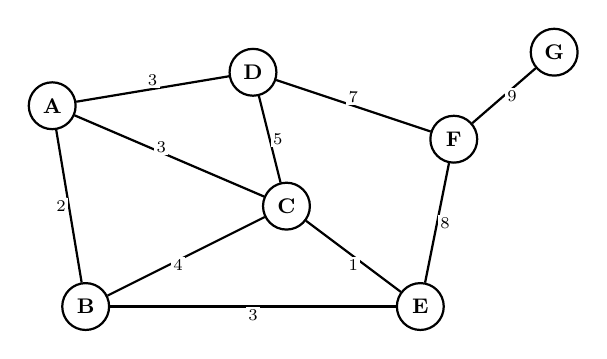
\begin{tikzpicture}[
  vertex/.style={circle, draw, thick, minimum size=7mm, font=\bfseries\small},
  edge label/.style={rectangle, draw=none, fill=white, font=\scriptsize, inner sep=1pt},
  scale=0.85, transform shape
]
  \node[vertex] (A) at (0, 3)   {A};
  \node[vertex] (D) at (3, 3.5)  {D};
  \node[vertex] (F) at (6, 2.5)  {F};
  \node[vertex] (G) at (7.5, 3.8){G};
  \node[vertex] (C) at (3.5, 1.5){C};
  \node[vertex] (B) at (0.5, 0)  {B};
  \node[vertex] (E) at (5.5, 0)  {E};
  \draw[thick] (A) -- node[edge label, above]       {3} (D);
  \draw[thick] (A) -- node[edge label, above left]   {3} (C);
  \draw[thick] (A) -- node[edge label, left]         {2} (B);
  \draw[thick] (D) -- node[edge label, right]        {5} (C);
  \draw[thick] (D) -- node[edge label, above]        {7} (F);
  \draw[thick] (C) -- node[edge label, below left]   {4} (B);
  \draw[thick] (C) -- node[edge label, below]        {1} (E);
  \draw[thick] (B) -- node[edge label, below]        {3} (E);
  \draw[thick] (E) -- node[edge label, right]        {8} (F);
  \draw[thick] (F) -- node[edge label, right]        {9} (G);
\end{tikzpicture}
\captionof{figure}{(a) Đồ thị gốc $G$ -- 10 cạnh}\label{fig:kruskal-graph}
\end{minipage}%
\hfill
\begin{minipage}[t]{0.48\textwidth}
\centering
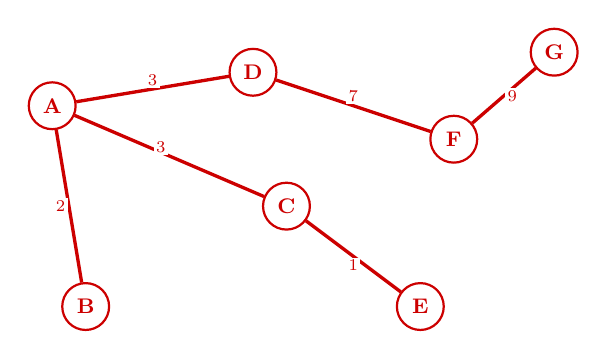
\begin{tikzpicture}[
  vertex/.style={circle, draw=red!80!black, thick, text=red!80!black, minimum size=7mm, font=\bfseries\small},
  edge label/.style={rectangle, draw=none, fill=white, font=\scriptsize, inner sep=1pt, text=red!80!black},
  scale=0.85, transform shape
]
  \node[vertex] (A) at (0, 3)   {A};
  \node[vertex] (D) at (3, 3.5)  {D};
  \node[vertex] (F) at (6, 2.5)  {F};
  \node[vertex] (G) at (7.5, 3.8){G};
  \node[vertex] (C) at (3.5, 1.5){C};
  \node[vertex] (B) at (0.5, 0)  {B};
  \node[vertex] (E) at (5.5, 0)  {E};
  % Only MST edges: CE(1), AB(2), AC(3), AD(3), DF(7), FG(9)
  \draw[very thick, red!80!black] (C) -- node[edge label, below]   {1} (E);
  \draw[very thick, red!80!black] (A) -- node[edge label, left]    {2} (B);
  \draw[very thick, red!80!black] (A) -- node[edge label, above left]{3} (C);
  \draw[very thick, red!80!black] (A) -- node[edge label, above]   {3} (D);
  \draw[very thick, red!80!black] (D) -- node[edge label, above]   {7} (F);
  \draw[very thick, red!80!black] (F) -- node[edge label, right]   {9} (G);
\end{tikzpicture}
\captionof{figure}{(b) MST kết quả -- 6 cạnh, tổng = 25}\label{fig:kruskal-mst}
\end{minipage}
\end{center}

Cho đồ thị $G$ với $V = \{A, B, C, D, E, F, G\}$ và các cạnh:

\begin{center}
\begin{tabular}{|c|c|c|c|c|c|c|c|c|c|c|}
\hline
Cạnh & CE & AB & AC & AD & BE & BC & CD & DF & EF & FG \\
\hline
$w$ & 1 & 2 & 3 & 3 & 3 & 4 & 5 & 7 & 8 & 9 \\
\hline
\end{tabular}
\end{center}

\textit{(Lưu ý: đồ thị Kruskal video không có cạnh CF -- khác với đồ thị Prim video bên dưới.)}

Sắp xếp cạnh theo $w$ tăng dần: \textbf{CE(1), AB(2), AC(3), AD(3), BE(3), BC(4), CD(5), DF(7), EF(8), FG(9)}.

Ban đầu: $\{A\}, \{B\}, \{C\}, \{D\}, \{E\}, \{F\}, \{G\}$. Cần $|V|-1 = 6$ cạnh.

\begin{center}
\renewcommand{\arraystretch}{1.5}
\begin{tabular}{|c|c|p{7.3cm}|c|}
\hline
\textbf{Bước} & \textbf{Cạnh (w)} & \textbf{Trạng thái Disjoint Sets} & \textbf{Cạnh $\to$ MST?} \\
\hline
1 & \textbf{CE} (1) & $\{A\},\{B\},\{C\},\{D\},\{E\},\{F\},\{G\}$ \newline $C$ và $E$ khác tập $\to$ \textbf{Union(C,E)} & \cellcolor{green!15} \textbf{Thêm vào MST} \\
\hline
2 & \textbf{AB} (2) & $\{A\},\{B\},\{C,E\},\{D\},\{F\},\{G\}$ \newline $A$ và $B$ khác tập $\to$ \textbf{Union(A,B)} & \cellcolor{green!15} \textbf{Thêm vào MST} \\
\hline
3 & \textbf{AC} (3) & $\{A,B\},\{C,E\},\{D\},\{F\},\{G\}$ \newline $A\in\{A,B\}$, $C\in\{C,E\}$ khác $\to$ \textbf{Union(A,C)} & \cellcolor{green!15} \textbf{Thêm vào MST} \\
\hline
4 & \textbf{AD} (3) & $\{A,B,C,E\},\{D\},\{F\},\{G\}$ \newline $A\in\{A,B,C,E\}$, $D\in\{D\}$ khác $\to$ \textbf{Union(A,D)} & \cellcolor{green!15} \textbf{Thêm vào MST} \\
\hline
5 & \textbf{BE} (3) & $\{A,B,C,D,E\},\{F\},\{G\}$ \newline \textcolor{red!80!black}{$B$ và $E$ cùng thuộc $\{A,B,C,D,E\}$ $\to$ Chu trình!} & \cellcolor{red!15} \textbf{Bỏ (chu trình)} \\
\hline
6 & \textbf{BC} (4) & $\{A,B,C,D,E\},\{F\},\{G\}$ \newline \textcolor{red!80!black}{Cùng tập $\to$ Chu trình!} & \cellcolor{red!15} \textbf{Bỏ (chu trình)} \\
\hline
7 & \textbf{CD} (5) & $\{A,B,C,D,E\},\{F\},\{G\}$ \newline \textcolor{red!80!black}{Cùng tập $\to$ Chu trình!} & \cellcolor{red!15} \textbf{Bỏ (chu trình)} \\
\hline
8 & \textbf{DF} (7) & $\{A,B,C,D,E\},\{F\},\{G\}$ \newline $D\in\{A,B,C,D,E\}$, $F\in\{F\}$ khác $\to$ \textbf{Union(D,F)} & \cellcolor{green!15} \textbf{Thêm vào MST} \\
\hline
9 & \textbf{EF} (8) & $\{A,B,C,D,E,F\},\{G\}$ \newline \textcolor{red!80!black}{Cùng tập $\to$ Chu trình!} & \cellcolor{red!15} \textbf{Bỏ (chu trình)} \\
\hline
10 & \textbf{FG} (9) & $\{A,B,C,D,E,F\},\{G\}$ \newline $F$ và $G$ khác tập $\to$ \textbf{Union(F,G)} & \cellcolor{green!15} \textbf{Thêm vào MST} \\
\hline
\multicolumn{4}{|c|}{$\{A,B,C,D,E,F,G\}$ -- $|F|=6=|V|-1$ $\to$ \textbf{DỪNG}.} \\
\hline
\end{tabular}
\captionof{table}{Kruskal -- Trace từng bước trên đồ thị mẫu}\label{tab:kruskal-trace}
\end{center}
\vspace{0.3cm}

\textbf{MST:} $\{CE, AB, AC, AD, DF, FG\}$, tổng = $1+2+3+3+7+9 = \boxed{25}$.

\subsubsection{\texorpdfstring{Prim (CLRS
\S 23.2)}{Prim (CLRS 23.2)}}\label{prim-clrs-23.2}

\textbf{Ý tưởng:} Mở rộng cây từ đỉnh \(s\), mỗi bước thêm cạnh nhẹ nhất
nối cây ra ngoài.

\begin{tcolorbox}[colback=gray!8, colframe=gray!50, boxrule=0.5pt, arc=2pt,
  left=6pt, right=6pt, top=4pt, bottom=4pt,
  title={\small\textbf{Pseudocode 14: Prim's Algorithm}}]
\begin{verbatim}
Prim(G, w, s):
    for moi u in V:
        key[u] = INF
        pi[u] = NIL
    key[s] = 0
    Q = MinPriorityQueue(V, key)
    while Q != empty:
        u = ExtractMin(Q)
        for moi v in Adj[u]:
            if v in Q and w(u,v) < key[v]:
                pi[v] = u
                key[v] = w(u,v)        // DecreaseKey
    return {(v, pi[v]) : v in V - {s}}
\end{verbatim}
\end{tcolorbox}

\begin{tcolorbox}[colback=yellow!5, colframe=orange!50, boxrule=0.5pt, arc=2pt, title={\small\textbf{Phân tích Complexity -- Prim's Algorithm}}]
\begin{tabular}{|l|l|l|}
\hline
\textbf{Dòng code} & \textbf{Số lần chạy} & \textbf{Chi phí} \\
\hline
\texttt{for u in V: key[u]=INF} & $V$ & $O(V)$ khởi tạo \\
\hline
\texttt{Q = MinPriorityQueue(V)} & 1 & $O(V)$ build heap \\
\hline
\texttt{u = ExtractMin(Q)} & $V$ lần & $O(\lg V)$ mỗi lần \\
\hline
\texttt{for v in Adj[u]:} & tổng $= 2E$ & mỗi cạnh xét 2 lần \\
\hline
\quad \texttt{DecreaseKey(v)} & tối đa $E$ lần & $O(\lg V)$ mỗi lần \\
\hline
\end{tabular}
\vspace{0.2cm}

\textbf{Time} (Min-Heap): $V \cdot O(\lg V)$ ExtractMin + $E \cdot O(\lg V)$ DecreaseKey $\to$ $O((V+E)\lg V) = O(E\lg V)$.\\
{\small (Nếu dùng Fibonacci Heap: DecreaseKey $O(1)$ amortized $\to$ $O(E + V\lg V)$.)}\\
\textbf{Space:} Mảng \texttt{key[V]}, \texttt{$\pi$[V]}, Priority Queue $Q$ chứa $V$ đỉnh $\to$ $O(V)$.
\end{tcolorbox}

\textbf{Chứng minh đúng (CLRS):} Cut (cây đang xây, đỉnh chưa thêm) luôn
được respect. Cạnh \((u,v)\) chọn là nhẹ nhất qua cut \(\to\) safe edge.
(OK)

\textbf{Complexity:} \(O(E \lg V)\) dùng binary heap. \(O(E + V \lg V)\)
dùng Fibonacci heap.

%=============================================
\textbf{Minh họa trực quan Prim (Visual Trace, bắt đầu từ $A$, đồ thị 7 đỉnh -- giống YouTube video):}

\begin{center}
\textit{Video hướng dẫn:} \href{https://www.youtube.com/watch?v=cplfcGZmX7I}{\textcolor{blue}{\underline{Prim's Algorithm -- YouTube (click để xem)}}}
\end{center}

\begin{center}
\begin{minipage}[t]{0.48\textwidth}
\centering
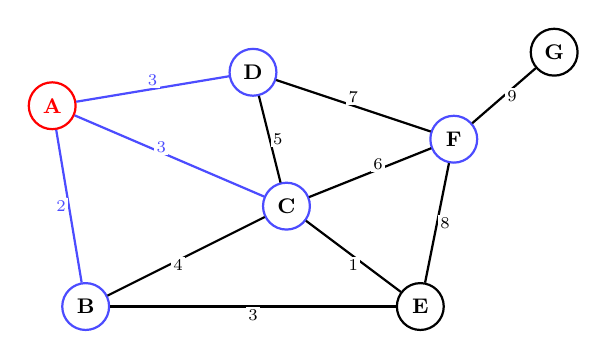
\begin{tikzpicture}[
  vertex/.style={circle, draw, thick, minimum size=7mm, font=\bfseries\small},
  edge label/.style={rectangle, draw=none, fill=white, font=\scriptsize, inner sep=1pt},
  scale=0.85, transform shape
]
  \node[vertex, draw=red, text=red] (A) at (0, 3)   {A};
  \node[vertex, draw=blue!70] (D) at (3, 3.5)  {D};
  \node[vertex, draw=blue!70] (F) at (6, 2.5)  {F};
  \node[vertex] (G) at (7.5, 3.8){G};
  \node[vertex, draw=blue!70] (C) at (3.5, 1.5){C};
  \node[vertex, draw=blue!70] (B) at (0.5, 0)  {B};
  \node[vertex] (E) at (5.5, 0)  {E};
  \draw[thick, blue!70] (A) -- node[edge label, above]       {3} (D);
  \draw[thick, blue!70] (A) -- node[edge label, above left]   {3} (C);
  \draw[thick, blue!70] (A) -- node[edge label, left]         {2} (B);
  \draw[thick] (D) -- node[edge label, right]        {5} (C);
  \draw[thick] (D) -- node[edge label, above]        {7} (F);
  \draw[thick] (C) -- node[edge label, below left]   {4} (B);
  \draw[thick] (C) -- node[edge label, below]        {1} (E);
  \draw[thick] (C) -- node[edge label, above right]  {6} (F);
  \draw[thick] (B) -- node[edge label, below]        {3} (E);
  \draw[thick] (E) -- node[edge label, right]        {8} (F);
  \draw[thick] (F) -- node[edge label, right]        {9} (G);
\end{tikzpicture}
\captionof{figure}{(a) Đồ thị gốc $G$ -- 11 cạnh. Visited=$\{A\}$}\label{fig:prim-graph}
\end{minipage}%
\hfill
\begin{minipage}[t]{0.48\textwidth}
\centering
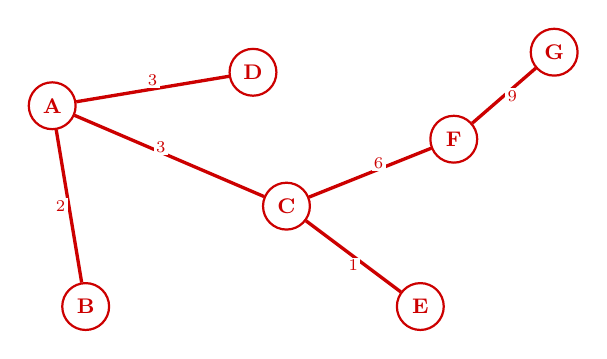
\begin{tikzpicture}[
  vertex/.style={circle, draw=red!80!black, thick, text=red!80!black, minimum size=7mm, font=\bfseries\small},
  edge label/.style={rectangle, draw=none, fill=white, font=\scriptsize, inner sep=1pt, text=red!80!black},
  scale=0.85, transform shape
]
  \node[vertex] (A) at (0, 3)   {A};
  \node[vertex] (D) at (3, 3.5)  {D};
  \node[vertex] (F) at (6, 2.5)  {F};
  \node[vertex] (G) at (7.5, 3.8){G};
  \node[vertex] (C) at (3.5, 1.5){C};
  \node[vertex] (B) at (0.5, 0)  {B};
  \node[vertex] (E) at (5.5, 0)  {E};
  % Prim MST edges: AB(2), AC(3), AD(3), CE(1), CF(6), FG(9)
  \draw[very thick, red!80!black] (A) -- node[edge label, left]    {2} (B);
  \draw[very thick, red!80!black] (A) -- node[edge label, above left]{3} (C);
  \draw[very thick, red!80!black] (A) -- node[edge label, above]   {3} (D);
  \draw[very thick, red!80!black] (C) -- node[edge label, below]   {1} (E);
  \draw[very thick, red!80!black] (C) -- node[edge label, above right]{6} (F);
  \draw[very thick, red!80!black] (F) -- node[edge label, right]   {9} (G);
\end{tikzpicture}
\captionof{figure}{(b) MST kết quả -- 6 cạnh, tổng = 24}\label{fig:prim-mst}
\end{minipage}
\end{center}

Cho đồ thị $G$ với $V = \{A, B, C, D, E, F, G\}$ và các cạnh:

\begin{center}
\begin{tabular}{|c|c|c|c|c|c|c|c|c|c|c|c|}
\hline
Cạnh & CE & AB & AC & AD & BE & BC & CD & CF & DF & EF & FG \\
\hline
$w$ & 1 & 2 & 3 & 3 & 3 & 4 & 5 & 6 & 7 & 8 & 9 \\
\hline
\end{tabular}
\end{center}

Ý tưởng then chốt: duy trì tập Visited ($S$) và Unvisited. Tại mỗi bước, tìm \textbf{cạnh bắt ngang} nhỏ nhất nối $S \to V\setminus S$ rồi thêm đỉnh mới vào $S$.

\begin{center}
\renewcommand{\arraystretch}{1.5}
\begin{tabular}{|c|c|p{6.5cm}|c|}
\hline
\textbf{Bước} & \textbf{Visited ($S$)} & \textbf{Cạnh bắt ngang (Crossing Edges)} & \textbf{Chọn (Min)} \\
\hline
0 & $\{A\}$ & \textbf{AB}(2), AC(3), AD(3). & \cellcolor{green!15} \textbf{AB} (2) \\
\hline
1 & $\{A,B\}$ & \textbf{AC}(3), AD(3), BE(3), BC(4). \newline \textit{(AB nằm trong $S$ $\to$ bỏ)} & \cellcolor{green!15} \textbf{AC} (3) \\
\hline
2 & $\{A,B,C\}$ & \textbf{CE}(1), AD(3), BE(3), BC(4), CD(5), CF(6). \newline \textit{(C mới đem vào cạnh: CE(1), CD(5), CF(6))} & \cellcolor{green!15} \textbf{CE} (1) \\
\hline
3 & $\{A,B,C,E\}$ & \textbf{AD}(3), BE(3), CD(5), CF(6), EF(8). \newline \textcolor{red!80!black}{\textit{BC, AC trong $S$ $\to$ loại. BE: B trong $S$, E trong $S$ $\to$ loại}} & \cellcolor{green!15} \textbf{AD} (3) \\
\hline
4 & $\{A,B,C,D,E\}$ & \textbf{CF}(6), DF(7), EF(8). \newline \textcolor{red!80!black}{\textit{CD, AD trong $S$ $\to$ loại. Thêm DF(7) từ D}} & \cellcolor{green!15} \textbf{CF} (6) \\
\hline
5 & $\{A,B,C,D,E,F\}$ & \textbf{FG}(9). \newline \textit{(DF, EF nằm trong $S$ $\to$ loại)} & \cellcolor{green!15} \textbf{FG} (9) \\
\hline
6 & $\{A,B,C,D,E,F,G\}$ & $|S|=7=|V|$ $\to$ \textbf{DỪNG}. & -- \\
\hline
\end{tabular}
\captionof{table}{Prim -- Trace từng bước trên đồ thị mẫu}\label{tab:prim-trace}
\end{center}
\vspace{0.3cm}

\textbf{MST:} $\{AB, AC, CE, AD, CF, FG\}$, tổng = $2+3+1+3+6+9 = \boxed{24}$. \textit{(Lưu ý: đồ thị Prim video có thêm cạnh CF(6) so với Kruskal video, nên MST khác: Prim chọn CF(6) thay vì DF(7), tổng 24 thay vì 25.)}

\subsubsection{So sánh trực diện Kruskal vs Prim}\label{so-sanh-kruskal-prim}

\begin{center}
\renewcommand{\arraystretch}{1.4}
\begin{tabular}{|p{3.2cm}|p{5.5cm}|p{5.5cm}|}
\hline
\textbf{Tiêu chí} & \textbf{Kruskal} & \textbf{Prim} \\
\hline
\textbf{Chiến lược} & Duyệt \textbf{cạnh} nhỏ nhất \textbf{toàn cục}, thêm nếu không tạo chu trình & Mở rộng \textbf{cây} từ 1 đỉnh, chọn cạnh nhẹ nhất \textbf{nối ra ngoài cây} \\
\hline
\textbf{Cấu trúc dữ liệu} & \textbf{Union-Find} (Disjoint Sets) & \textbf{Min-Priority Queue} \\
\hline
\textbf{Bước đầu tiên} & Sắp xếp tất cả cạnh theo $w$ & Chọn đỉnh bắt đầu $s$ \\
\hline
\textbf{Kiểm tra chu trình} & FindSet($u$) $\neq$ FindSet($v$)? & Đỉnh $v$ chưa trong cây? ($v \in Q$?) \\
\hline
\textbf{Complexity} & $O(E \lg V)$ (sort + Union-Find) & $O(E \lg V)$ (binary heap) \newline $O(E + V \lg V)$ (Fibonacci heap) \\
\hline
\textbf{Phù hợp khi} & Đồ thị \textbf{thưa} ($E \approx V$) & Đồ thị \textbf{dày} ($E \approx V^2$) \\
\hline
\textbf{Cần sắp xếp cạnh?} & \textbf{Có} (toàn bộ $E$ cạnh) & \textbf{Không} \\
\hline
\textbf{Chứng minh đúng} & Cut Theorem: cạnh nhẹ nhất qua cut giữa 2 component & Cut Theorem: cạnh nhẹ nhất qua cut (cây, phần còn lại) \\
\hline
\textbf{MST forests} & Xây nhiều cây rồi hợp nhất & Luôn xây \textbf{1 cây duy nhất} \\
\hline
\end{tabular}
\captionof{table}{So sánh Kruskal và Prim -- Đặc điểm và Ưu điểm}\label{tab:kruskal-vs-prim}
\end{center}


\begin{traceyourself}{Kruskal -- Trace từ đầu}
Cho đồ thị 4 đỉnh $\{1,2,3,4\}$ với cạnh: $(1,2,w{=}4)$, $(1,3,w{=}1)$, $(2,3,w{=}3)$, $(2,4,w{=}2)$, $(3,4,w{=}5)$.

Sắp xếp cạnh tăng dần: \underline{\hspace{8cm}}

\begin{center}
\begin{tabular}{|c|c|c|c|c|}
\hline
\textbf{Bước} & \textbf{Cạnh} & \textbf{$w$} & \textbf{Chu trình?} & \textbf{Kết quả} \\
\hline
1 & \underline{\hspace{2cm}} & \underline{\hspace{1cm}} & \underline{\hspace{2cm}} & \underline{\hspace{4cm}} \\
\hline
2 & \underline{\hspace{2cm}} & \underline{\hspace{1cm}} & \underline{\hspace{2cm}} & \underline{\hspace{4cm}} \\
\hline
3 & \underline{\hspace{2cm}} & \underline{\hspace{1cm}} & \underline{\hspace{2cm}} & \underline{\hspace{4cm}} \\
\hline
\end{tabular}
\end{center}

Tổng trọng số MST = \underline{\hspace{2cm}}
\end{traceyourself}

\whyprompt{Tại sao cạnh nhẹ nhất qua một cut \textbf{phải} thuộc MST? Thử dùng phản chứng: giả sử cạnh nhẹ nhất $(u,v)$ qua cut KHÔNG thuộc MST $T^*$. Thêm $(u,v)$ vào $T^*$ tạo ra gì? Điều gì xảy ra?}

\begin{center}\rule{0.5\linewidth}{0.5pt}\end{center}

\section{Chương 6: Đường đi Ngắn nhất -- Shortest Paths: Dijkstra (CLRS Ch.24)}\label{chux1b0ux1a1ng-6-ux111ux1b0ux1eddng-ux111i-ngux1eafn-nhux1ea5t-dijkstra-clrs-ch.24}

\intuition{GPS tìm đường đi ngắn nhất chính là Dijkstra (hoặc A*). Ý tưởng: luôn \textbf{xử lý đỉnh gần nhất trước} (Greedy), rồi cập nhật (relax) các hàng xóm. Mỗi đỉnh khi được ``khóa'' vào tập $S$ sẽ không bao giờ bị cập nhật lại -- đây là bất biến cốt lõi của Dijkstra. Kết hợp tư duy Greedy (chọn min) và DP (relaxation = cập nhật bảng).}

\pitfall{(1) \textbf{Dijkstra KHÔNG hoạt động với cạnh âm} -- phải dùng Bellman-Ford. (2) Khởi tạo $d[s] = 0$, $d[v] = \infty$ (không phải $-\infty$ hay $0$). (3) Khi có nhiều đỉnh cùng khoảng cách minimun, chọn bất kỳ đều đúng -- không ảnh hưởng kết quả. (4) Dijkstra cho \textbf{single-source} -- nếu cần all-pairs hãy dùng Floyd-Warshall.}

\subsection{\texorpdfstring{Bài toán (CLRS
\S 24.0)}{Bài toán (CLRS 24.0)}}\label{buxe0i-touxe1n-clrs-24.0}

Cho \(G = (V, E, w)\) có hướng, \(w: E \to \mathbb{R}^+\). Đỉnh nguồn
\(s\).

\textbf{3 biến thể:}

\begin{enumerate}
\def\labelenumi{\arabic{enumi}.}
\tightlist
\item
  \textbf{Single-pair:} \(s \to t\)
\item
  \textbf{Single-source:} \(s \to\) tất cả \(v\) -- \textbf{(Dijkstra)}
\item
  \textbf{All-pairs:} mọi \(u \to v\) -- \textbf{(Floyd-Warshall)}
\end{enumerate}

\textbf{Tính chất cấu trúc tối ưu (CLRS Lemma 24.1):}

\begin{quote}
Mọi đường đi con của đường đi ngắn nhất cũng là đường đi ngắn nhất.
\end{quote}

\subsection{\texorpdfstring{Relaxation (CLRS \S 24.3) -- Kỹ thuật
cốt
lõi}{Relaxation (CLRS 24.3) -- Kỹ thuật cốt lõi}}\label{relaxation-clrs-24.3-kux1ef9-thuux1eadt-cux1ed1t-luxf5i}

\begin{tcolorbox}[colback=gray!8, colframe=gray!50, boxrule=0.5pt, arc=2pt,
  left=6pt, right=6pt, top=4pt, bottom=4pt,
  title={\small\textbf{Pseudocode 15: Relaxation}}]
\begin{verbatim}
Relax(u, v, w):
    if d[v] > d[u] + w(u,v):
        d[v] = d[u] + w(u,v)
        pi[v] = u
\end{verbatim}
\end{tcolorbox}

\(d[v]\) = \textbf{ước lượng trên} (upper bound) cho \(\delta(s,v)\).
Relaxation chỉ \textbf{giảm} \(d[v]\).

\subsection{\texorpdfstring{Thuật toán Dijkstra (CLRS
\S 24.3)}{Thuật toán Dijkstra (CLRS 24.3)}}\label{thuux1eadt-touxe1n-dijkstra-clrs-24.3}

% ===== DIJKSTRA PSEUDOCODE WITH ANNOTATIONS =====
\begin{center}
\begin{tikzpicture}[remember picture]
\node[text width=0.55\linewidth, anchor=north west, inner sep=0] (code) at (0,0) {
\begin{lstlisting}[escapechar=|]
Dijkstra(G, w, s):
    for moi v in V:|\tikzmark{init}|
        d[v] = INF;  pi[v] = NIL
    d[s] = 0|\tikzmark{source}|
    S = empty
    Q = MinPriorityQueue(V, d)|\tikzmark{queue}|
    while Q != empty:
        u = ExtractMin(Q)|\tikzmark{greedy}|
        S = S + {u}
        for moi v in Adj[u]:|\tikzmark{relax}|
            Relax(u, v, w)
\end{lstlisting}
};

% Right-side annotations with arrows
\node[text width=4.8cm, anchor=west, font=\small\itshape, text=blue!70!black]
  (n1) at ([xshift=0.56\linewidth, yshift=-0.3cm]code.north west)
  {Khởi tạo mọi đỉnh: khoảng cách $= \infty$, cha $=$ NIL};
\draw[-{Stealth[length=4pt]}, blue!50, thick]
  (n1.west) -- ([xshift=0.54\linewidth, yshift=-0.3cm]code.north west);

\node[text width=4.8cm, anchor=west, font=\small\itshape, text=green!60!black]
  (n2) at ([xshift=0.56\linewidth, yshift=-1.1cm]code.north west)
  {Đỉnh nguồn có $d[s]=0$ -- điểm xuất phát};
\draw[-{Stealth[length=4pt]}, green!50!black, thick]
  (n2.west) -- ([xshift=0.54\linewidth, yshift=-1.1cm]code.north west);

\node[text width=4.8cm, anchor=west, font=\small\itshape, text=red!70!black]
  (n3) at ([xshift=0.56\linewidth, yshift=-2.1cm]code.north west)
  {\textbf{GREEDY:} Luôn chọn đỉnh gần nhất -- bất biến cốt lõi};
\draw[-{Stealth[length=4pt]}, red!60, thick]
  (n3.west) -- ([xshift=0.54\linewidth, yshift=-2.1cm]code.north west);

\node[text width=4.8cm, anchor=west, font=\small\itshape, text=violet!70!black]
  (n4) at ([xshift=0.56\linewidth, yshift=-3.0cm]code.north west)
  {\textbf{DP update:} Cập nhật $d[v]$ nếu tìm đường ngắn hơn qua $u$};
\draw[-{Stealth[length=4pt]}, violet!60, thick]
  (n4.west) -- ([xshift=0.54\linewidth, yshift=-3.0cm]code.north west);
\end{tikzpicture}
\end{center}

\subsubsection{Chứng minh đúng đắn (CLRS Theorem
24.6):}\label{chux1ee9ng-minh-ux111uxfang-ux111ux1eafn-clrs-theorem-24.6}

\textbf{Theorem:} Khi \(u\) được thêm vào \(S\) (extracted from Q):
\(d[u] = \delta(s,u)\).

\textbf{Chứng minh (phản chứng -- CLRS style):}

\begin{itemize}
\tightlist
\item
  Giả sử \(u\) là đỉnh \textbf{đầu tiên} thêm vào \(S\) mà
  \(d[u] \neq \delta(s,u)\) \(\to\) \(d[u] > \delta(s,u)\)
\item
  Xét đường đi ngắn nhất \(s \leadsto x \to y \leadsto u\), trong đó
  \(x \in S, y \notin S\)
\item
  Vì \(x\) đã được xử lý: \(d[x] = \delta(s,x)\) \(\to\) sau relax:
  \(d[y] = \delta(s,y)\)
\item
  Vì \(u\) được chọn trước \(y\) (ExtractMin): \(d[u] \leq d[y]\)
\item
  Mà \(d[y] = \delta(s,y) \leq \delta(s,u) \leq d[u]\) (vì \(w \geq 0\))
\item
  \(\to\) \(d[u] = \delta(s,u)\) \textbf{mâu thuẫn!} (OK)
\end{itemize}

\begin{quote}
\textbf{Điều kiện:} \(w(u,v) \geq 0\) cho mọi cạnh. Nếu có trọng số âm
\(\to\) dùng \textbf{Bellman-Ford}.
\end{quote}

\subsubsection{Minh họa trực quan Dijkstra (Visual Trace -- đồ thị giống video YouTube):}

\begin{center}
\textit{Video hướng dẫn:} \href{https://www.youtube.com/watch?v=_lHSawdgXpI}{\textcolor{blue}{\underline{Dijkstra's Algorithm -- YouTube (click để xem)}}}
\end{center}

Cho đồ thị \textbf{có hướng} $G$ với $V = \{A, B, C, D, E\}$, nguồn $s = A$:

\begin{center}
\begin{tabular}{|c|c|c|c|c|c|c|c|c|c|}
\hline
Cạnh & A$\to$B & A$\to$C & B$\to$C & B$\to$D & B$\to$E & C$\to$B & C$\to$D & C$\to$E & E$\to$D \\
\hline
$w$ & 4 & 2 & 3 & 2 & 3 & 1 & 4 & 5 & 1 \\
\hline
\end{tabular}
\captionof{table}{Dijkstra -- Danh sách cạnh đồ thị mẫu}\label{tab:dijkstra-edges}
\end{center}

\begin{center}
\begin{minipage}[t]{0.48\textwidth}
\centering
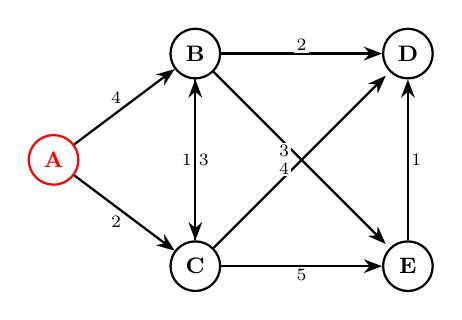
\begin{tikzpicture}[
  vertex/.style={circle, draw, thick, minimum size=7mm, font=\bfseries\small},
  edge label/.style={rectangle, draw=none, fill=white, font=\scriptsize, inner sep=1pt},
  >=Stealth, scale=0.9, transform shape
]
  \node[vertex, draw=red, text=red] (A) at (0, 1.5) {A};
  \node[vertex] (B) at (2, 3)   {B};
  \node[vertex] (C) at (2, 0)   {C};
  \node[vertex] (D) at (5, 3)   {D};
  \node[vertex] (E) at (5, 0)   {E};
  % Directed edges
  \draw[->, thick] (A) -- node[edge label, above left] {4} (B);
  \draw[->, thick] (A) -- node[edge label, below left] {2} (C);
  \draw[->, thick] (B) -- node[edge label, right] {3} (C);
  \draw[->, thick] (B) -- node[edge label, above] {2} (D);
  \draw[->, thick, shorten >=2pt] (B) -- node[edge label, below, pos=0.4] {3} (E);
  \draw[->, thick] (C) -- node[edge label, left] {1} (B);
  \draw[->, thick, shorten >=2pt] (C) -- node[edge label, above, pos=0.4] {4} (D);
  \draw[->, thick] (C) -- node[edge label, below] {5} (E);
  \draw[->, thick] (E) -- node[edge label, right] {1} (D);
\end{tikzpicture}
\captionof{figure}{(a) Đồ thị gốc $G$ -- 9 cạnh có hướng}\label{fig:dijkstra-graph}
\end{minipage}%
\hfill
\begin{minipage}[t]{0.48\textwidth}
\centering
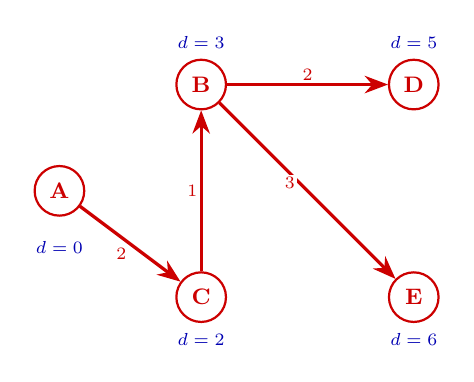
\begin{tikzpicture}[
  vertex/.style={circle, draw=red!80!black, thick, text=red!80!black, minimum size=7mm, font=\bfseries\small},
  edge label/.style={rectangle, draw=none, fill=white, font=\scriptsize, inner sep=1pt, text=red!80!black},
  >=Stealth, scale=0.9, transform shape
]
  \node[vertex] (A) at (0, 1.5) {A};
  \node[vertex] (B) at (2, 3)   {B};
  \node[vertex] (C) at (2, 0)   {C};
  \node[vertex] (D) at (5, 3)   {D};
  \node[vertex] (E) at (5, 0)   {E};
  % Shortest path tree edges only
  \draw[->, very thick, red!80!black] (A) -- node[edge label, below left] {2} (C);
  \draw[->, very thick, red!80!black] (C) -- node[edge label, left] {1} (B);
  \draw[->, very thick, red!80!black] (B) -- node[edge label, above] {2} (D);
  \draw[->, very thick, red!80!black] (B) -- node[edge label, below, pos=0.4] {3} (E);
  % Distance labels
  \node[font=\scriptsize\bfseries, text=blue!70!black] at (0, 0.7) {$d=0$};
  \node[font=\scriptsize\bfseries, text=blue!70!black] at (2, 3.6) {$d=3$};
  \node[font=\scriptsize\bfseries, text=blue!70!black] at (2, -0.6) {$d=2$};
  \node[font=\scriptsize\bfseries, text=blue!70!black] at (5, 3.6) {$d=5$};
  \node[font=\scriptsize\bfseries, text=blue!70!black] at (5, -0.6) {$d=6$};
\end{tikzpicture}
\captionof{figure}{(b) Cây đường đi ngắn nhất từ $A$}\label{fig:dijkstra-spt}
\end{minipage}
\end{center}

\textbf{Trace Dijkstra từ $s = A$:}

\begin{center}
\begin{tabular}{|c|c|c|c|c|c|c|l|}
\hline
\textbf{Bước} & $d[A]$ & $d[B]$ & $d[C]$ & $d[D]$ & $d[E]$ & \textbf{ExtractMin} & \textbf{Relaxation} \\
\hline
Init & \cellcolor{green!15}\textbf{[0]} & $\infty$ & $\infty$ & $\infty$ & $\infty$ & $A$ & -- \\
\hline
1 & 0 & 4 & \cellcolor{green!15}\textbf{[2]} & $\infty$ & $\infty$ & $C$ & \small A$\to$B: $d[B]=4$, A$\to$C: $d[C]=2$ \\
\hline
2 & 0 & \cellcolor{green!15}\textbf{[3]} & 2 & 6 & 7 & $B$ & \small C$\to$B: $\min(4, 2{+}1){=}3$, C$\to$D: $6$, C$\to$E: $7$ \\
\hline
3 & 0 & 3 & 2 & \cellcolor{green!15}\textbf{[5]} & 6 & $D$ & \small B$\to$D: $\min(6, 3{+}2){=}5$, B$\to$E: $\min(7, 3{+}3){=}6$ \\
\hline
4 & 0 & 3 & 2 & 5 & \cellcolor{green!15}\textbf{[6]} & $E$ & \small E$\to$D: $6{+}1{=}7 > 5$, no change \\
\hline
\end{tabular}
\captionof{table}{Dijkstra -- Bảng trace khoảng cách từng bước}\label{tab:dijkstra-trace}
\end{center}

\textbf{Kết quả:} $d[A]=0$, $d[B]=3$, $d[C]=2$, $d[D]=5$, $d[E]=6$.

\textbf{Đường đi ngắn nhất:}
\begin{itemize}
\tightlist
\item $A \to C$: chi phí $= 2$ (trực tiếp)
\item $A \to C \to B$: chi phí $= 2 + 1 = 3$
\item $A \to C \to B \to D$: chi phí $= 2 + 1 + 2 = 5$
\item $A \to C \to B \to E$: chi phí $= 2 + 1 + 3 = 6$
\end{itemize}

\subsubsection{\texorpdfstring{Complexity (CLRS
\S 24.3):}{Complexity (CLRS 24.3):}}\label{complexity-clrs-24.3}

\(O(V \lg V + E)\) (Fibonacci heap) hoặc \(O((V+E) \lg V)\) (binary
heap)

\whyprompt{Tại sao Dijkstra \textbf{không hoạt động} với cạnh có trọng số âm? Hãy tự xây dựng một \textbf{phản ví dụ} (3 đỉnh, 1 cạnh âm) mà Dijkstra cho kết quả sai.}

\begin{traceyourself}{Dijkstra -- Trace bảng khoảng cách}
Cho đồ thị có hướng 4 đỉnh $\{s,a,b,t\}$ với cạnh: $s{\to}a(1)$, $s{\to}b(4)$, $a{\to}b(2)$, $a{\to}t(6)$, $b{\to}t(3)$.

\begin{center}
\begin{tabular}{|c|c|c|c|c|c|}
\hline
\textbf{Bước} & $d[s]$ & $d[a]$ & $d[b]$ & $d[t]$ & \textbf{ExtractMin} \\
\hline
Init & \textbf{[0]} & $\infty$ & $\infty$ & $\infty$ & $s$ \\
\hline
1 & 0 & \underline{\hspace{1.5cm}} & \underline{\hspace{1.5cm}} & \underline{\hspace{1.5cm}} & \underline{\hspace{1.5cm}} \\
\hline
2 & 0 & \underline{\hspace{1.5cm}} & \underline{\hspace{1.5cm}} & \underline{\hspace{1.5cm}} & \underline{\hspace{1.5cm}} \\
\hline
3 & 0 & \underline{\hspace{1.5cm}} & \underline{\hspace{1.5cm}} & \underline{\hspace{1.5cm}} & \underline{\hspace{1.5cm}} \\
\hline
\end{tabular}
\end{center}

Đường đi ngắn nhất $s \to t$: \underline{\hspace{4cm}}, chi phí = \underline{\hspace{2cm}}
\end{traceyourself}


\begin{center}\rule{0.5\linewidth}{0.5pt}\end{center}

\section{Chương 7: Quy hoạch Động -- Dynamic Programming (CLRS Ch.14)}\label{chux1b0ux1a1ng-7-quy-houx1ea1ch-ux111ux1ed9ng-dp-clrs-ch.14}

\intuition{DP = \textbf{``Nhớ để không tính lại''}. Nếu đệ quy ngây thơ giải Fibonacci tốn $O(2^n)$ vì tính trùng lắp, thì DP chỉ tốn $O(n)$ bằng cách lưu kết quả vào bảng. Khi nào dùng DP? Khi bài toán có \textbf{optimal substructure} và \textbf{overlapping subproblems} -- hai tính chất quan trọng nhất. Floyd-Warshall và Matrix Chain Multiplication là hai ví dụ điển hình.}

\pitfall{(1) DP chỉ đúng nếu có optimal substructure -- không phải mọi bài ``chia nhỏ'' đều dùng DP được. (2) Trong Pascal/binomial coefficient DP, \textbf{phải duyệt $j$ từ lớn đến nhỏ} (downto) để tránh dùng giá trị đã cập nhật trong cùng vòng lặp $i$. (3) Floyd-Warshall cần khởi tạo đường chéo $D[i][i] = 0$, không phải $\infty$.}


\subsection{Ý tưởng Quy hoạch Động (Dynamic Programming)}\label{y-tuong-dp}

Quy hoạch Động (DP) giải bài toán tối ưu bằng cách \textbf{chia thành bài toán con chồng lấp} (overlapping subproblems), giải mỗi bài con \textbf{đúng 1 lần}, lưu kết quả vào bảng để tái sử dụng.

\textbf{Khi nào dùng DP?} Khi bài toán có 2 tính chất:
\begin{enumerate}
\item \textbf{Optimal substructure:} Nghiệm tối ưu bài toán lớn \textit{chứa} nghiệm tối ưu bài toán con.
\item \textbf{Overlapping subproblems:} Các bài toán con được gọi lại nhiều lần (đệ quy ngây thơ sẽ tính lại $\to$ lãng phí).
\end{enumerate}

\textbf{Hai phương pháp triển khai:}
\begin{itemize}
\item \textbf{Top-down (Memoization):} Viết đệ quy + cache. Dễ code nhưng overhead gọi hàm.
\item \textbf{Bottom-up (Tabulation):} Điền bảng từ bài toán nhỏ $\to$ lớn. Hiệu quả hơn, không cần stack đệ quy.
\end{itemize}

\textbf{So sánh D\&C vs DP:} D\&C chia thành bài toán con \textit{không chồng lấp} (independent), DP chia thành bài toán con \textit{chồng lấp} (shared). Nếu có overlapping mà dùng D\&C thẳng $\to$ exponential time (vd: Fibonacci naive $O(2^n)$).

\subsection{\texorpdfstring{Bốn bước thiết kế DP (CLRS
\S 14.1)}{Bốn bước thiết kế DP (CLRS 14.1)}}\label{bux1ed1n-bux1b0ux1edbc-thiux1ebft-kux1ebf-dp-clrs-14.1}

\begin{enumerate}
\def\labelenumi{\arabic{enumi}.}
\tightlist
\item
  \textbf{Characterize} cấu trúc nghiệm tối ưu (optimal substructure)
\item
  \textbf{Define} giá trị nghiệm tối ưu bằng đệ quy
\item
  \textbf{Compute} giá trị nghiệm tối ưu bottom-up (hoặc top-down +
  memo)
\item
  \textbf{Construct} nghiệm tối ưu từ thông tin đã tính
\end{enumerate}

\subsection{\texorpdfstring{Hai tính chất then chốt (CLRS
\S 14.3)}{Hai tính chất then chốt (CLRS 14.3)}}\label{hai-tuxednh-chux1ea5t-then-chux1ed1t-clrs-14.3}

\subsubsection{(1) Optimal Substructure:}\label{optimal-substructure}

\begin{quote}
Nghiệm tối ưu của bài toán \textbf{chứa} nghiệm tối ưu của bài toán con.
\end{quote}

\subsubsection{(2) Overlapping
Subproblems:}\label{overlapping-subproblems}

\begin{quote}
Các bài toán con \textbf{trùng lặp} (gọi đi gọi lại) \(\to\) lưu bảng
thay vì tính lại.
\end{quote}

\subsubsection{So sánh: Tham lam -- Chia để trị -- Quy hoạch động}\label{greedy-dc-dp}

\begin{center}
{\small
\begin{longtable}{|>{\raggedright\arraybackslash}p{2.2cm}|>{\raggedright\arraybackslash}p{3.8cm}|>{\raggedright\arraybackslash}p{3.8cm}|>{\raggedright\arraybackslash}p{3.8cm}|}
\hline
\textbf{Tiêu chí} & \textbf{Tham lam (Greedy)} & \textbf{Chia để trị (D\&C)} & \textbf{Quy hoạch động (DP)} \\
\hline\hline
\textbf{Ý tưởng} & Luôn chọn phương án \textbf{tốt nhất tại chỗ}, hy vọng dẫn đến tối ưu toàn cục & \textbf{Chia} thành bài con \textbf{độc lập}, giải đệ quy, rồi \textbf{gộp} kết quả & Chia thành bài con \textbf{chồng lấp}, giải \textbf{đúng 1 lần}, lưu bảng tái sử dụng \\
\hline
\textbf{Bài toán con} & Không chia rõ ràng -- chỉ giảm kích thước sau mỗi chọn & \textbf{Tách biệt} (disjoint) -- không giao nhau & \textbf{Chồng lấp} (overlapping) -- cùng bài con xuất hiện nhiều lần \\
\hline
\textbf{Tính chất cần} & Greedy-choice property + Optimal substructure & Chia được thành bài con nhỏ cùng dạng & Optimal substructure + Overlapping subproblems \\
\hline
\textbf{Thứ tự quyết định} & \textbf{Trước} khi giải bài con (top-down, không quay lui) & Giải bài con \textbf{trước}, gộp sau & Giải \textbf{tất cả} bài con, sau đó chọn tối ưu \\
\hline
\textbf{Cách giải} & Vòng lặp đơn giản (sort + chọn) & Đệ quy trực tiếp & Tabulation (bottom-up) / Memoization (top-down) \\
\hline
\textbf{Time phổ biến} & $O(n \lg n)$ & $O(n \lg n)$ & $O(n^2)$ hoặc $O(n^3)$ \\
\hline
\textbf{Khi nào dùng?} & Tối ưu + chứng minh được Greedy-choice & Bài con \textbf{độc lập} nhau & Tối ưu + bài con chồng lấp, \textit{không} có Greedy-choice \\
\hline
\textbf{Ví dụ} & Kruskal, Prim, Dijkstra, Activity Selection & Merge Sort, Quick Sort, Binary Search & Fibonacci, Floyd-Warshall, MCM, 0/1 Knapsack \\
\hline
\end{longtable}
}
\captionof{table}{So sánh ba phương pháp thiết kế thuật toán}\label{tab:greedy-dc-dp}
\end{center}

\subsection{\texorpdfstring{Pascal -- Tổ hợp
\(C(n,k)\)}{Pascal -- Tổ hợp C(n,k)}}\label{pascal-tux1ed5-hux1ee3p-cnk}

\(C(n,k) = C(n-1,k) + C(n-1,k-1)\), \(\quad C(n,0) = C(n,n) = 1\)

\subsubsection{\texorpdfstring{Thuật toán 1: \(O(nk)\) time, \(O(nk)\)
space}{Thuật toán 1: O(nk) time, O(nk) space}}\label{thuux1eadt-touxe1n-1-onk-time-onk-space}

\begin{tcolorbox}[colback=gray!8, colframe=gray!50, boxrule=0.5pt, arc=2pt,
  left=6pt, right=6pt, top=4pt, bottom=4pt,
  title={\small\textbf{Pseudocode 17: Pascal Triangle -- DP (O(nk) space)}}]
\begin{verbatim}
Pascal1(n, k):
    C[0..n][0..k]
    for i = 0 to n:
        for j = 0 to min(i, k):
            if j = 0 or j = i: C[i][j] = 1
            else: C[i][j] = C[i-1][j] + C[i-1][j-1]
    return C[n][k]
\end{verbatim}
\end{tcolorbox}

\begin{tcolorbox}[colback=yellow!5, colframe=orange!50, boxrule=0.5pt, arc=2pt, title={\small\textbf{Phân tích Complexity -- Pascal Triangle DP ($O(nk)$ space)}}]
\begin{tabular}{|l|l|l|}
\hline
\textbf{Dòng code} & \textbf{Số lần chạy} & \textbf{Chi phí} \\
\hline
\texttt{C[0..n][0..k]} khởi tạo & $(n+1)(k+1)$ & cấp phát bảng 2D \\
\hline
\texttt{for i = 0 to n} & $n+1$ & vòng ngoài \\
\hline
\quad \texttt{for j = 0 to min(i,k)} & $\sum_{i=0}^{n}\min(i,k)+1$ & vòng trong \\
\hline
\quad\quad \texttt{C[i][j] = C[i-1][j] + C[i-1][j-1]} & $\leq nk$ & $\Theta(1)$ mỗi ô \\
\hline
\end{tabular}
\vspace{0.2cm}

\textbf{Time:} 2 vòng lồng: $i$ chạy $n+1$ lần, $j$ chạy tối đa $\min(i,k)$ $\to$ tổng $\leq n \cdot k$ ô $\to$ $O(nk)$.\\
\textbf{Space:} Bảng 2D $C[0..n][0..k]$ có $(n+1)(k+1)$ ô $\to$ $O(nk)$.
\end{tcolorbox}

\subsubsection{\texorpdfstring{Thuật toán 2: \(O(nk)\) time, \(O(k)\)
space -- TỐI
ƯU}{Thuật toán 2: O(nk) time, O(k) space -- TỐI ƯU}}\label{thuux1eadt-touxe1n-2-onk-time-ok-space-tux1ed1i-ux1b0u}

\begin{tcolorbox}[colback=gray!8, colframe=gray!50, boxrule=0.5pt, arc=2pt,
  left=6pt, right=6pt, top=4pt, bottom=4pt,
  title={\small\textbf{Pseudocode 18: Pascal Triangle -- DP tối ưu (O(k) space)}}]
\begin{verbatim}
Pascal2(n, k):
    C[0..k], C[0] = 1
    for i = 1 to n:
        for j = min(i,k) downto 1:     // !!! PHAI duyet nguoc!
            C[j] = C[j] + C[j-1]
    return C[k]
\end{verbatim}
\end{tcolorbox}

\begin{tcolorbox}[colback=yellow!5, colframe=orange!50, boxrule=0.5pt, arc=2pt, title={\small\textbf{Phân tích Complexity -- Pascal Triangle DP tối ưu ($O(k)$ space)}}]
\begin{tabular}{|l|l|l|}
\hline
\textbf{Dòng code} & \textbf{Số lần chạy} & \textbf{Chi phí} \\
\hline
\texttt{C[0..k], C[0] = 1} & $k+1$ & cấp phát mảng 1D \\
\hline
\texttt{for i = 1 to n} & $n$ & vòng ngoài \\
\hline
\quad \texttt{for j = min(i,k) downto 1} & $\leq nk$ & \textbf{duyệt ngược} (quan trọng!) \\
\hline
\quad\quad \texttt{C[j] = C[j] + C[j-1]} & $\leq nk$ & $\Theta(1)$ mỗi lần \\
\hline
\end{tabular}
\vspace{0.2cm}

\textbf{Time:} Vẫn $O(nk)$ -- cùng số phép tính như cách 1.\\
\textbf{Space:} Chỉ dùng 1 mảng $C[0..k]$ $\to$ $O(k)$! \textit{Tối ưu từ $O(nk)$ xuống $O(k)$ nhờ duyệt \textbf{ngược} $j$.}\\
{\small (Duyệt ngược đảm bảo $C[j-1]$ chưa bị ghi đè khi tính $C[j]$ -- giống kỹ thuật 0/1 Knapsack.)}
\end{tcolorbox}

\subsection{Floyd-Warshall -- Đường đi ngắn nhất mọi cặp đỉnh (CLRS
Ch.25)}\label{floyd-warshall-ux111ux1b0ux1eddng-ux111i-ngux1eafn-nhux1ea5t-mux1ecdi-cux1eb7p-ux111ux1ec9nh-clrs-ch.25}

\textbf{Input:} Ma trận \(L[n \times n]\), \(L[i][j] = w(v_i, v_j)\)
hoặc \(\infty\)

\textbf{Output:} Ma trận \(D[n \times n]\), \(D[i][j] = \delta(i,j)\) =
đường đi ngắn nhất \(i \to j\)

\textbf{Optimal substructure:} Đường đi ngắn nhất \(i \to j\) qua tập
đỉnh trung gian \(\{1..k\}\) hoặc đi qua \(k\), hoặc không.

\begin{tcolorbox}[colback=gray!8, colframe=gray!50, boxrule=0.5pt, arc=2pt,
  left=6pt, right=6pt, top=4pt, bottom=4pt,
  title={\small\textbf{Pseudocode 19: Floyd-Warshall}}]
\begin{verbatim}
Floyd-Warshall(W):
    D = W
    for k = 1 to n:
        for i = 1 to n:
            for j = 1 to n:
                if D[i][j] > D[i][k] + D[k][j]:
                    D[i][j] = D[i][k] + D[k][j]
    return D
\end{verbatim}
\end{tcolorbox}

\begin{tcolorbox}[colback=yellow!5, colframe=orange!50, boxrule=0.5pt, arc=2pt, title={\small\textbf{Phân tích Complexity -- Floyd-Warshall}}]
\begin{tabular}{|l|l|l|}
\hline
\textbf{Dòng code} & \textbf{Số lần chạy} & \textbf{Chi phí} \\
\hline
\texttt{D = W} (copy ma trận) & $n^2$ & $\Theta(n^2)$ \\
\hline
\texttt{for k = 1 to n} & $n$ & vòng ngoài (đỉnh trung gian) \\
\hline
\quad \texttt{for i = 1 to n} & $n^2$ & vòng giữa \\
\hline
\quad\quad \texttt{for j = 1 to n} & $n^3$ & vòng trong \\
\hline
\quad\quad\quad \texttt{D[i][j] = min(...)} & $n^3$ & $\Theta(1)$ mỗi lần \\
\hline
\end{tabular}
\vspace{0.2cm}

\textbf{Time:} 3 vòng \texttt{for} lồng nhau, mỗi vòng $n$ lần $\to$ $n \times n \times n = \Theta(n^3)$.\\
\textbf{Space:} Ma trận $D[n \times n]$ $\to$ $\Theta(n^2)$. {\small (Có thể cập nhật in-place trên 1 ma trận vì $D^{(k)}[i][k] = D^{(k-1)}[i][k]$.)}
\end{tcolorbox}

\textbf{Ý nghĩa:} \(D^{(k)}[i][j]\) = đường đi ngắn nhất \(i \to j\) chỉ
dùng đỉnh trung gian \(\{1, \ldots, k\}\)

\textbf{Complexity:} \(\Theta(n^3)\) time, \(\Theta(n^2)\) space

\whyprompt{Trong Floyd-Warshall, tại sao vòng lặp $k$ \textbf{phải ở ngoài cùng}? Nếu đặt $i$ hoặc $j$ ở ngoài thì sao? Gợi ý: nghĩ về ``qua tập đỉnh trung gian $\{1..k\}$'' -- thứ tự xây bảng DP quan trọng!}

\subsubsection{Ví dụ minh họa: 4 đỉnh (giải đầy đủ)}\label{vd-floyd-4dinh}

\begin{center}
\begin{minipage}[t]{0.48\textwidth}
\centering
\textbf{Đồ thị ban đầu (Input)}

\vspace{0.3cm}
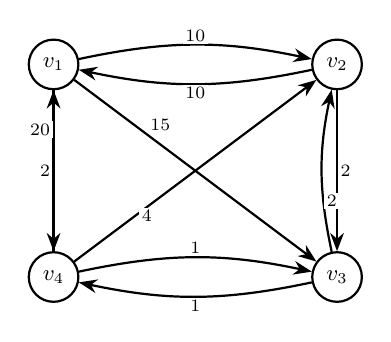
\begin{tikzpicture}[
  vertex/.style={circle, draw, thick, minimum size=7mm, font=\bfseries\small},
  edge label/.style={rectangle, draw=none, fill=white, font=\scriptsize, inner sep=1pt},
  >=Stealth, scale=0.9, transform shape
]
  \node[vertex] (v1) at (0, 3)   {$v_1$};
  \node[vertex] (v2) at (4, 3)   {$v_2$};
  \node[vertex] (v3) at (4, 0)   {$v_3$};
  \node[vertex] (v4) at (0, 0)   {$v_4$};

  % Edges with clear labels
  \draw[->, thick] (v1) to[bend left=12] node[edge label, above] {10} (v2);
  \draw[->, thick] (v2) to[bend left=12] node[edge label, below] {10} (v1);
  \draw[->, thick] (v1) -- node[edge label, pos=0.3, above right] {15} (v3);
  \draw[->, thick] (v1) -- node[edge label, left] {2} (v4);
  \draw[->, thick] (v2) -- node[edge label, right] {2} (v3);
  \draw[->, thick] (v3) to[bend left=12] node[edge label, below] {1} (v4);
  \draw[->, thick] (v4) to[bend left=12] node[edge label, above] {1} (v3);
  \draw[->, thick] (v3) to[bend left=12] node[edge label, right, pos=0.3] {2} (v2);
  \draw[->, thick] (v4) -- node[edge label, pos=0.7, above left] {20} (v1);
  \draw[->, thick] (v4) -- node[edge label, below, pos=0.3] {4} (v2);
\end{tikzpicture}
\captionof{figure}{(a) Đồ thị gốc -- 10 cạnh có hướng}\label{fig:floyd-graph}
\end{minipage}%
\hfill
\begin{minipage}[t]{0.48\textwidth}
\centering
\textbf{Shortest Paths từ $v_1$ (Output)}

\vspace{0.3cm}
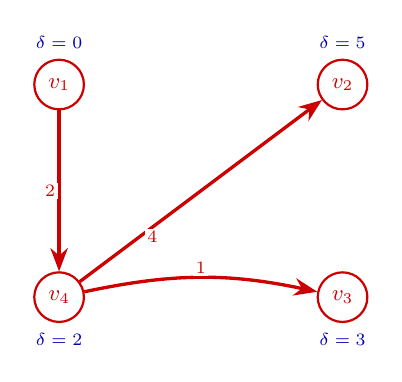
\begin{tikzpicture}[
  vertex/.style={circle, draw=red!80!black, thick, text=red!80!black, minimum size=7mm, font=\bfseries\small},
  edge label/.style={rectangle, draw=none, fill=white, font=\scriptsize, inner sep=1pt, text=red!80!black},
  >=Stealth, scale=0.9, transform shape
]
  \node[vertex] (v1) at (0, 3)   {$v_1$};
  \node[vertex] (v2) at (4, 3)   {$v_2$};
  \node[vertex] (v3) at (4, 0)   {$v_3$};
  \node[vertex] (v4) at (0, 0)   {$v_4$};

  % Shortest path edges only
  \draw[->, very thick, red!80!black] (v1) -- node[edge label, left] {2} (v4);
  \draw[->, very thick, red!80!black] (v4) -- node[edge label, below, pos=0.3] {4} (v2);
  \draw[->, very thick, red!80!black] (v4) to[bend left=12] node[edge label, above] {1} (v3);

  % Distance labels (blue, outside nodes)
  \node[font=\scriptsize\bfseries, text=blue!70!black] at (0, 3.6) {$\delta=0$};
  \node[font=\scriptsize\bfseries, text=blue!70!black] at (4, 3.6) {$\delta=5$};
  \node[font=\scriptsize\bfseries, text=blue!70!black] at (4, -0.6) {$\delta=3$};
  \node[font=\scriptsize\bfseries, text=blue!70!black] at (0, -0.6) {$\delta=2$};
\end{tikzpicture}
\captionof{figure}{(b) Cây đường đi ngắn nhất từ $v_1$}\label{fig:floyd-spt}

{\small $v_1{\to}v_4{\to}v_2{=}5$,\quad $v_1{\to}v_4{\to}v_3{=}3$}
\end{minipage}
\end{center}

\vspace{0.2cm}

Ma trận trọng số $L$ (input):

$$D^{(0)} = L = \begin{pmatrix} 0 & 10 & 15 & 2 \\ 10 & 0 & 2 & \infty \\ \infty & 2 & 0 & 1 \\ 20 & 4 & 1 & 0 \end{pmatrix}$$

\textbf{$k = 1$ (xét đỉnh trung gian $v_1$):} Kiểm tra $D[i][j]$ so với $D[i][1] + D[1][j]$.

$D[2][4] = \min(\infty, 10+2) = 12$, \quad $D[4][2] = \min(4, 20+10) = 4$ (không đổi)

$$D^{(1)} = \begin{pmatrix} 0 & 10 & 15 & 2 \\ 10 & 0 & 2 & 12 \\ \infty & 2 & 0 & 1 \\ 20 & 4 & 1 & 0 \end{pmatrix}$$

\textbf{$k = 2$ (qua $v_1, v_2$):}

$D[1][3] = \min(15, 10+2) = 12$, \quad $D[3][1] = \min(\infty, 2+10) = 12$

$D[3][4] = \min(1, 2+12) = 1$ (không đổi), \quad $D[4][3] = \min(1, 4+2) = 1$ (không đổi)

$$D^{(2)} = \begin{pmatrix} 0 & 10 & 12 & 2 \\ 10 & 0 & 2 & 12 \\ 12 & 2 & 0 & 1 \\ 20 & 4 & 1 & 0 \end{pmatrix}$$

\textbf{$k = 3$ (qua $v_1, v_2, v_3$):}

$D[1][4] = \min(2, 12+1) = 2$ (không đổi), \quad $D[2][4] = \min(12, 2+1) = 3$

$D[4][1] = \min(20, 1+12) = 13$, \quad $D[4][2] = \min(4, 1+2) = 3$

$$D^{(3)} = \begin{pmatrix} 0 & 10 & 12 & 2 \\ 10 & 0 & 2 & 3 \\ 12 & 2 & 0 & 1 \\ 13 & 3 & 1 & 0 \end{pmatrix}$$

\textbf{$k = 4$ (qua tất cả đỉnh):}

$D[1][2] = \min(10, 2+3) = 5$, \quad $D[1][3] = \min(12, 2+1) = 3$

$D[2][1] = \min(10, 3+13) = 10$ (không đổi), \quad $D[3][1] = \min(12, 1+13) = 12$ (không đổi)

$$\boxed{D^{(4)} = \begin{pmatrix} 0 & 5 & 3 & 2 \\ 10 & 0 & 2 & 3 \\ 12 & 2 & 0 & 1 \\ 13 & 3 & 1 & 0 \end{pmatrix}}$$

\textbf{Đọc kết quả:} $\delta(v_1, v_2) = 5$ (đi $v_1 \to v_4 \to v_2$), $\delta(v_1, v_3) = 3$ (đi $v_1 \to v_4 \to v_3$).

\subsubsection{Ví dụ 2: 4 đỉnh với cạnh âm}\label{vd-floyd-canh-am}

\textbf{Lưu ý:} Đồ thị này có \textbf{cạnh âm} ($-2$ và $-1$) -- Dijkstra \textbf{không hoạt động} nhưng Floyd-Warshall vẫn đúng!

\begin{center}
\begin{minipage}[t]{0.48\textwidth}
\centering
\textbf{Đồ thị ban đầu (Input)}

\vspace{0.3cm}
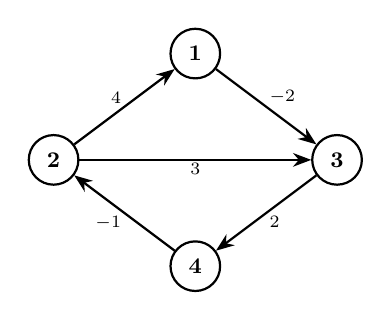
\begin{tikzpicture}[
  vertex/.style={circle, draw, thick, minimum size=7mm, font=\bfseries\small},
  edge label/.style={rectangle, draw=none, fill=white, font=\scriptsize, inner sep=1pt},
  >=Stealth, scale=0.9, transform shape
]
  \node[vertex] (v1) at (2, 3)   {1};
  \node[vertex] (v2) at (0, 1.5) {2};
  \node[vertex] (v3) at (4, 1.5) {3};
  \node[vertex] (v4) at (2, 0)   {4};

  \draw[->, thick] (v2) -- node[edge label, above left] {4} (v1);
  \draw[->, thick] (v1) -- node[edge label, above right] {$-2$} (v3);
  \draw[->, thick] (v2) -- node[edge label, below] {3} (v3);
  \draw[->, thick] (v3) -- node[edge label, below right] {2} (v4);
  \draw[->, thick] (v4) -- node[edge label, below left] {$-1$} (v2);
\end{tikzpicture}
\captionof{figure}{(a) Đồ thị có cạnh âm -- 5 cạnh}\label{fig:floyd2-graph}
\end{minipage}%
\hfill
\begin{minipage}[t]{0.48\textwidth}
\centering
\textbf{Shortest Paths từ đỉnh 1}

\vspace{0.3cm}
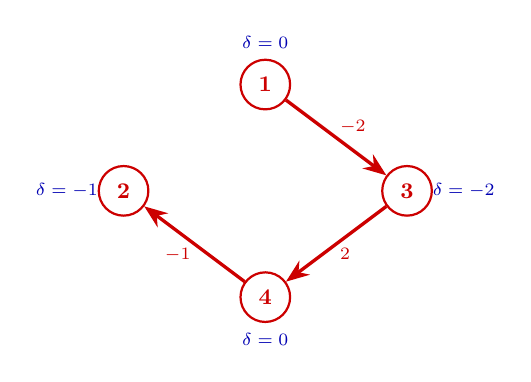
\begin{tikzpicture}[
  vertex/.style={circle, draw=red!80!black, thick, text=red!80!black, minimum size=7mm, font=\bfseries\small},
  edge label/.style={rectangle, draw=none, fill=white, font=\scriptsize, inner sep=1pt, text=red!80!black},
  >=Stealth, scale=0.9, transform shape
]
  \node[vertex] (v1) at (2, 3)   {1};
  \node[vertex] (v2) at (0, 1.5) {2};
  \node[vertex] (v3) at (4, 1.5) {3};
  \node[vertex] (v4) at (2, 0)   {4};

  % Shortest path edges
  \draw[->, very thick, red!80!black] (v1) -- node[edge label, above right] {$-2$} (v3);
  \draw[->, very thick, red!80!black] (v3) -- node[edge label, below right] {2} (v4);
  \draw[->, very thick, red!80!black] (v4) -- node[edge label, below left] {$-1$} (v2);

  % Distance labels
  \node[font=\scriptsize\bfseries, text=blue!70!black] at (2, 3.6) {$\delta=0$};
  \node[font=\scriptsize\bfseries, text=blue!70!black] at (-0.8, 1.5) {$\delta=-1$};
  \node[font=\scriptsize\bfseries, text=blue!70!black] at (4.8, 1.5) {$\delta=-2$};
  \node[font=\scriptsize\bfseries, text=blue!70!black] at (2, -0.6) {$\delta=0$};
\end{tikzpicture}
\captionof{figure}{(b) $1{\to}3{\to}4{\to}2 = {-1}$}\label{fig:floyd2-spt}
\end{minipage}
\end{center}

Ma trận trọng số $W$ (input), $\infty$ = không có cạnh:

$$D^{(0)} = W = \begin{pmatrix} 0 & \infty & -2 & \infty \\ 4 & 0 & 3 & \infty \\ \infty & \infty & 0 & 2 \\ \infty & -1 & \infty & 0 \end{pmatrix}$$

\textbf{$k = 1$ (qua đỉnh 1):}

$D[2][3] = \min(3, 4+(-2)) = \min(3, 2) = 2$

$$D^{(1)} = \begin{pmatrix} 0 & \infty & -2 & \infty \\ 4 & 0 & \mathbf{2} & \infty \\ \infty & \infty & 0 & 2 \\ \infty & -1 & \infty & 0 \end{pmatrix}$$

\textbf{$k = 2$ (qua đỉnh 1, 2):}

$D[4][1] = \min(\infty, {-1}+4) = 3$, \quad $D[4][3] = \min(\infty, {-1}+2) = 1$

$$D^{(2)} = \begin{pmatrix} 0 & \infty & -2 & \infty \\ 4 & 0 & 2 & \infty \\ \infty & \infty & 0 & 2 \\ \mathbf{3} & -1 & \mathbf{1} & 0 \end{pmatrix}$$

\textbf{$k = 3$ (qua đỉnh 1, 2, 3):}

$D[1][4] = \min(\infty, {-2}+2) = 0$, \quad $D[2][4] = \min(\infty, 2+2) = 4$

$$D^{(3)} = \begin{pmatrix} 0 & \infty & -2 & \mathbf{0} \\ 4 & 0 & 2 & \mathbf{4} \\ \infty & \infty & 0 & 2 \\ 3 & -1 & 1 & 0 \end{pmatrix}$$

\textbf{$k = 4$ (qua tất cả đỉnh):}

$D[1][2] = \min(\infty, 0+({-1})) = -1$, \quad $D[2][1] = \min(4, 4+3) = 4$ (không đổi)

$D[3][1] = \min(\infty, 2+3) = 5$, \quad $D[3][2] = \min(\infty, 2+({-1})) = 1$

$$\boxed{D^{(4)} = \begin{pmatrix} 0 & -1 & -2 & 0 \\ 4 & 0 & 2 & 4 \\ 5 & 1 & 0 & 2 \\ 3 & -1 & 1 & 0 \end{pmatrix}}$$

\textbf{Đọc kết quả từ đỉnh 1:} $\delta(1,2) = -1$ (đi $1 \to 3 \to 4 \to 2$), $\delta(1,3) = -2$ (đi $1 \to 3$), $\delta(1,4) = 0$ (đi $1 \to 3 \to 4$).

\textit{Nhận xét:} Đường đi ngắn nhất có thể \textbf{âm} nhờ cạnh âm. Floyd-Warshall xử lý đúng vì xét \textit{tất cả} đỉnh trung gian, không Greedy.

\begin{center}\rule{0.5\linewidth}{0.5pt}\end{center}

\section{Chương 8: Nhân Chuỗi Ma trận -- Matrix Chain Multiplication (CLRS \S 14.2)}\label{chux1b0ux1a1ng-8-nhuxe2n-chuux1ed7i-ma-trux1eadn-clrs-14.2}

\intuition{Nhân ma trận có tính kết hợp: $(AB)C = A(BC)$. Nhưng \textbf{chi phí tính toán} lại phụ thuộc cách đặt ngoặc! Đây là bài toán tối ưu hóa thuần túy -- không thể Greedy (không có greedy-choice đơn giản) -- phải DP. Ta điền bảng $m[i][j]$ theo thứ tự tăng dần độ dài chain, từng bước xây dựng lên nghiệm tối ưu.}

\pitfall{(1) Chỉ số $p$ có $n+1$ phần tử cho $n$ ma trận: $p = \langle p_0, p_1, \ldots, p_n \rangle$. (2) Điền bảng \textbf{theo chain length} ($l = 2, 3, \ldots, n$) -- không phải theo thứ tự $i, j$. (3) $m[i][j]$ lưu \textbf{số phép nhân scalar}, không phải số phép nhân ma trận.}

\subsection{8.1 Bài toán}\label{buxe0i-touxe1n}

Cho dãy ma trận \(\langle A_1, A_2, \ldots, A_n \rangle\), \(A_i\) có
kích thước \(p_{i-1} \times p_i\). Tìm cách đặt ngoặc để \textbf{tổng số
phép nhân đơn vị} nhỏ nhất.

\textbf{Ví dụ:} \(A(3 \times 100)\), \(B(100 \times 50)\),
\(C(50 \times 20)\):

\begin{itemize}
\tightlist
\item
  \((AB)C = 15{,}000 + 3{,}000 = 18{,}000\) (tốt)
\item
  \(A(BC) = 100{,}000 + 6{,}000 = 106{,}000\) (xấu)
\end{itemize}

\subsection{\texorpdfstring{Phân tích DP (CLRS
\S 14.2)}{Phân tích DP (CLRS 14.2)}}\label{phuxe2n-tuxedch-dp-clrs-14.2}

\textbf{Optimal substructure:} Nếu đặt ngoặc tối ưu chia tại \(k\):
\((A_i \ldots A_k)(A_{k+1} \ldots A_j)\), thì mỗi phần cũng phải được
đặt ngoặc tối ưu.

\textbf{Công thức:}
\[
m[i][j] = \begin{cases} 0 & \text{nếu } i = j \\ \displaystyle\min_{i \leq k < j} \left\{ m[i][k] + m[k+1][j] + p_{i-1} \cdot p_k \cdot p_j \right\} & \text{nếu } i < j \end{cases}
\]

\textbf{Số Catalan:} Số cách đặt ngoặc
\(= C(n) = \Omega(4^n / n^{3/2})\) \(\to\) brute force \textbf{không khả
thi}.

\subsubsection{Thuật toán (CLRS):}\label{thuux1eadt-touxe1n-clrs}

\begin{tcolorbox}[colback=gray!8, colframe=gray!50, boxrule=0.5pt, arc=2pt,
  left=6pt, right=6pt, top=4pt, bottom=4pt,
  title={\small\textbf{Pseudocode 20: Matrix Chain Multiplication}}]
\begin{verbatim}
MatrixChainOrder(p):
    n = len(p) - 1
    m[1..n][1..n],  s[1..n][1..n]
    for i = 1 to n: m[i][i] = 0
    for l = 2 to n:                    // chain length
        for i = 1 to n-l+1:
            j = i + l - 1
            m[i][j] = INF
            for k = i to j-1:
                q = m[i][k] + m[k+1][j] + p[i-1] * p[k] * p[j]
                if q < m[i][j]:
                    m[i][j] = q
                    s[i][j] = k        // luu split point
    return m, s

PrintOptimalParens(s, i, j):
    if i = j: print "A_i"
    else:
        print "("
        PrintOptimalParens(s, i, s[i][j])
        PrintOptimalParens(s, s[i][j]+1, j)
        print ")"
\end{verbatim}
\end{tcolorbox}

\begin{tcolorbox}[colback=yellow!5, colframe=orange!50, boxrule=0.5pt, arc=2pt, title={\small\textbf{Phân tích Complexity -- Matrix Chain Multiplication}}]
\begin{tabular}{|l|l|l|}
\hline
\textbf{Dòng code} & \textbf{Số lần chạy} & \textbf{Chi phí} \\
\hline
\texttt{m[1..n][1..n], s[1..n][1..n]} & $2n^2$ & cấp phát 2 bảng \\
\hline
\texttt{for i = 1 to n: m[i][i]=0} & $n$ & khởi tạo đường chéo \\
\hline
\texttt{for l = 2 to n} & $n-1$ & chain length (vòng ngoài) \\
\hline
\quad \texttt{for i = 1 to n-l+1} & $\sum_{l=2}^{n}(n-l+1)$ & vòng giữa \\
\hline
\quad\quad \texttt{for k = i to j-1} & $\sum_{l=2}^{n}\sum_{i}(l-1)$ & vòng trong (thử split) \\
\hline
\quad\quad\quad \texttt{q = m[i][k]+m[k+1][j]+p...} & mỗi lần $\Theta(1)$ & 1 phép cộng + nhân \\
\hline
\end{tabular}
\vspace{0.2cm}

\textbf{Tính tổng vòng lặp:}
\[\sum_{l=2}^{n}\sum_{i=1}^{n-l+1}(l-1) = \sum_{l=2}^{n}(n-l+1)(l-1) = \Theta(n^3)\]
{\small (Đây là tổ hợp $\binom{n}{3}$ -- số cách chọn 3 chỉ số từ $n$.)}

\textbf{Time:} 3 vòng lồng nhau $\to$ $\Theta(n^3)$.\\
\textbf{Space:} Bảng $m[n \times n]$ + $s[n \times n]$ $\to$ $\Theta(n^2)$.
\end{tcolorbox}

\subsubsection{Ví dụ minh họa: 3 ma trận}\label{vd-mcm-3matrix}

Cho $A_1(10 \times 30)$, $A_2(30 \times 5)$, $A_3(5 \times 60)$. Vậy $p = \langle 10, 30, 5, 60 \rangle$.

\textbf{Chain dài 2 ($l = 2$):}

$m[1][2] = p_0 \cdot p_1 \cdot p_2 = 10 \times 30 \times 5 = 1500, \quad s[1][2] = 1$

$m[2][3] = p_1 \cdot p_2 \cdot p_3 = 30 \times 5 \times 60 = 9000, \quad s[2][3] = 2$

\textbf{Chain dài 3 ($l = 3$):}

$m[1][3] = \min\begin{cases} k{=}1: m[1][1] + m[2][3] + p_0 p_1 p_3 = 0 + 9000 + 10 \times 30 \times 60 = 27000 \\ k{=}2: m[1][2] + m[3][3] + p_0 p_2 p_3 = 1500 + 0 + 10 \times 5 \times 60 = 4500 \end{cases}$

$m[1][3] = \boxed{4500}, \quad s[1][3] = 2$

\textbf{Bảng $m$:}
\begin{center}
\begin{tabular}{|c|c|c|c|}
\hline
$m$ & 1 & 2 & 3 \\
\hline
1 & 0 & 1500 & \textbf{4500} \\
\hline
2 & & 0 & 9000 \\
\hline
3 & & & 0 \\
\hline
\end{tabular}
\end{center}

\textbf{Thứ tự tối ưu:} $s[1][3] = 2$, nên chia $(A_1 A_2)(A_3) = \boxed{(A_1 A_2) A_3}$.

Chi phí: nhân $A_1 A_2$ tốn $1500$, kết quả $10 \times 5$; rồi nhân với $A_3$ tốn $10 \times 5 \times 60 = 3000$. Tổng: $4500$.

So sánh: $A_1(A_2 A_3)$ tốn $9000 + 18000 = 27000$ -- \textbf{gấp 6 lần!}

\begin{center}\rule{0.5\linewidth}{0.5pt}\end{center}

\section{Chương 9: Lý thuyết Độ phức tạp -- P, NP, NP-Complete (CLRS Ch.34)}\label{chux1b0ux1a1ng-9-p-np-np-complete-clrs-ch.34}

\intuition{P vs NP là câu hỏi mở lớn nhất của khoa học máy tính (và là 1 trong 7 bài toán Millennium Prize). Trực giác: P = ``giải được nhanh'', NP = ``kiểm tra được nhanh''. Chứng minh một bài toán NP-Complete có nghĩa là \textbf{không ai} tìm được thuật toán polynomial cho nó -- một kết quả tiêu cực nhưng rất hữu ích, vì ta biết nên chuyển sang tìm approximation thay vì tìm nghiệm chính xác.}

\pitfall{(1) NP không có nghĩa là ``Non-Polynomial'' -- NP = Nondeterministic Polynomial (kiểm tra được trong poly time). (2) $P \subseteq NP$ nhưng ta chưa biết $P = NP$ hay $P \neq NP$. (3) Để chứng minh $L$ là NP-Complete, phải chứng minh cả 2 điều: $L \in NP$ VÀ có reduction từ một bài NPC đã biết vào $L$ (không phải từ $L$ ra).}

\subsection{9.1 Lớp P}\label{lux1edbp-p}

\begin{quote}
\textbf{P} = \{bài toán quyết định giải được trong \(O(n^k)\) cho hằng
số \(k\)\}
\end{quote}

Ví dụ: Sorting \(O(n \lg n)\), MST \(O(E \lg V)\), Shortest path
\(O(V \lg V + E)\)

\subsection{9.2 Lớp NP}\label{lux1edbp-np}

\begin{quote}
\textbf{NP} = \{bài toán quyết định mà \textbf{lời giải kiểm tra được}
trong polynomial time\}
\end{quote}

\begin{itemize}
\tightlist
\item
  Cho certificate (lời giải), verifier kiểm tra trong \(O(n^k)\)
\item
  \(P \subseteq NP\) (hiển nhiên: giải được \(\to\) kiểm tra được)
\item
  \(P = NP\)? \(\to\) Câu hỏi mở lớn nhất của CS!
\end{itemize}

\subsection{\texorpdfstring{Polynomial Reduction (CLRS
\S 34.3)}{Polynomial Reduction (CLRS 34.3)}}\label{polynomial-reduction-clrs-34.3}

\(A \leq_p B\) (\(A\) quy về \(B\)): Có hàm \(f\) tính trong polynomial
time sao cho: \[x \in A \Longleftrightarrow f(x) \in B\]

\textbf{Ý nghĩa:} \(B\) \textbf{ít nhất khó bằng} \(A\). Nếu giải \(B\)
được \(\to\) giải \(A\) được.

\subsection{\texorpdfstring{NP-Complete (CLRS
\S 34.4)}{NP-Complete (CLRS 34.4)}}\label{np-complete-clrs-34.4}

Bài toán \(L\) là \textbf{NP-Complete} nếu:

\begin{enumerate}
\def\labelenumi{\arabic{enumi}.}
\tightlist
\item
  \(L \in NP\)
\item
  \(\forall L' \in NP\): \(L' \leq_p L\) (mọi bài toán NP đều quy về
  \(L\))
\end{enumerate}

\textbf{Ví dụ:} Hamilton Cycle -- đi qua tất cả đỉnh đúng 1 lần, quay
về.

\begin{itemize}
\tightlist
\item
  \(\in NP\): cho chu trình, kiểm tra \(O(n)\)
\item
  Chưa có thuật toán polynomial để \textbf{tìm} \(\to\) NP-Complete
\item
  Nếu ai giải được Hamilton trong P \(\to\) \(P = NP\) !
\end{itemize}

\textbf{Cách chứng minh NPC (CLRS \S 34.4):}

\begin{enumerate}
\def\labelenumi{\arabic{enumi}.}
\tightlist
\item
  Chứng minh \(L \in NP\)
\item
  Chọn bài NPC đã biết \(L'\) (SAT, 3-SAT, CLIQUE, VERTEX-COVER,
  HAMILTONIAN-CYCLE\ldots)
\item
  Chứng minh \(L' \leq_p L\) (polynomial reduction)
\item
  \(\to\) \(L\) là NP-Complete (OK)
\end{enumerate}

\feynman{Giải thích P vs NP cho bà ngoại bạn. Gợi ý: ``P = bài toán mà máy tính giải NHANH. NP = bài toán mà máy tính KIỂM TRA lời giải nhanh. Câu hỏi triệu đô: có phải mọi bài kiểm tra nhanh đều giải nhanh?'' -- Nếu bạn giải thích được rõ hơn thế, bạn đã hiểu.}

\checkpoint{Để chứng minh bài toán $L$ là NP-Complete, ta cần reduce TỪ bài NPC đã biết $L'$ VÀO $L$ (tức $L' \leq_p L$). Tại sao chiều reduction quan trọng? Nếu reduce ngược ($L \leq_p L'$) thì ta chứng minh được điều gì?}

\whyprompt{Tại sao một số bài toán \textbf{không thể giải được trong thời gian đa thức} (polynomial time)? Nếu P $\neq$ NP, điều đó có ý nghĩa gì cho thực tiễn? Gợi ý: nghĩ về số lượng nghiệm cần kiểm tra và tại sao ``kiểm tra nhanh'' không đồng nghĩa với ``tìm nhanh''.}

\begin{center}\rule{0.5\linewidth}{0.5pt}\end{center}

\newpage
\section{Chương 10: Bài tập Mẫu có Lời giải -- Practice Problems with Solutions}\label{bai-tap-mau}

%=============================================
\subsection{Bài 1: Độ phức tạp -- Master Theorem}

\textbf{Đề bài:} Giải các công thức đệ quy sau:
\begin{enumerate}
\item[(a)] $T(n) = 4T(n/2) + n$
\item[(b)] $T(n) = 2T(n/2) + n \lg n$
\item[(c)] $T(n) = 3T(n/4) + n \lg n$
\end{enumerate}

\textbf{Lời giải:}

\textbf{(a)} $T(n) = 4T(n/2) + n$

$a = 4, \quad b = 2, \quad \log_b a = \log_2 4 = 2$

$f(n) = n = O(n^{2-\varepsilon})$ với $\varepsilon = 1$. Vì $f(n)$ tăng chậm hơn $n^2$:

$\to$ \textbf{Case 1:} $T(n) = \Theta(n^{\log_2 4}) = \boxed{\Theta(n^2)}$

\textbf{(b)} $T(n) = 2T(n/2) + n \lg n$

$a = 2, \quad b = 2, \quad \log_b a = 1$

$f(n) = n \lg n = \Theta(n^1 \cdot \lg^1 n)$ với $k = 1$.

$\to$ \textbf{Case 2:} $T(n) = \Theta(n^1 \cdot \lg^{1+1} n) = \boxed{\Theta(n \lg^2 n)}$

\textbf{(c)} $T(n) = 3T(n/4) + n \lg n$

$a = 3, \quad b = 4, \quad \log_4 3 \approx 0.793$

$f(n) = n \lg n = \Omega(n^{0.793 + \varepsilon})$ với $\varepsilon \approx 0.2$.

Kiểm tra regularity: $3 \cdot (n/4)\lg(n/4) = (3/4) n \lg(n/4) \leq (3/4) n \lg n = c \cdot f(n)$ với $c = 3/4 < 1$. (OK)

$\to$ \textbf{Case 3:} $T(n) = \Theta(f(n)) = \boxed{\Theta(n \lg n)}$

%=============================================
\subsection{Bài 2: QuickSort -- Trace Partition}

\textbf{Đề bài:} Cho mảng $A = [7, 2, 1, 6, 8, 5, 3, 4]$. Thực hiện Partition với pivot = $A[8] = 4$. Cho biết trạng thái mảng sau mỗi bước.

\textbf{Lời giải:}

Pivot $= A[8] = 4$, $i = 0$ (trước $p$).

\begin{center}
\begin{tabular}{|c|c|c|l|}
\hline
\textbf{j} & \textbf{A[j]} & \textbf{So sánh} & \textbf{Mảng sau bước} \\
\hline
1 & 7 & $7 > 4$ $\to$ skip & $[7, 2, 1, 6, 8, 5, 3, \mathbf{4}]$, $i=0$ \\
\hline
2 & 2 & $2 \leq 4$ $\to$ $i{=}1$, swap $A[1] \leftrightarrow A[2]$ & $[\mathbf{2}, 7, 1, 6, 8, 5, 3, 4]$, $i=1$ \\
\hline
3 & 1 & $1 \leq 4$ $\to$ $i{=}2$, swap $A[2] \leftrightarrow A[3]$ & $[2, \mathbf{1}, 7, 6, 8, 5, 3, 4]$, $i=2$ \\
\hline
4 & 6 & $6 > 4$ $\to$ skip & không đổi, $i=2$ \\
\hline
5 & 8 & $8 > 4$ $\to$ skip & không đổi, $i=2$ \\
\hline
6 & 5 & $5 > 4$ $\to$ skip & không đổi, $i=2$ \\
\hline
7 & 3 & $3 \leq 4$ $\to$ $i{=}3$, swap $A[3] \leftrightarrow A[7]$ & $[2, 1, \mathbf{3}, 6, 8, 5, 7, 4]$, $i=3$ \\
\hline
\end{tabular}
\end{center}

Swap cuối: $A[i+1] \leftrightarrow A[r]$ = $A[4] \leftrightarrow A[8]$:

$$A = [2, 1, 3, \boxed{4}, 8, 5, 7, 6]$$

Kết quả: pivot $4$ ở vị trí $q = 4$.
\begin{itemize}
\tightlist
\item Bên trái ($A[1..3] = [2, 1, 3]$): tất cả $\leq 4$ (OK)
\item Bên phải ($A[5..8] = [8, 5, 7, 6]$): tất cả $> 4$ (OK)
\end{itemize}

\textbf{Complexity:} Partition duyệt $n-1$ phần tử $\to$ $\Theta(n)$.

%=============================================

%=============================================
\subsection{Bài 4: Dijkstra -- Đường đi ngắn nhất}

\textbf{Đề bài:} Cho đồ thị có hướng $G$ với 5 đỉnh $\{s, a, b, c, t\}$ và các cạnh:

\begin{center}
\begin{tabular}{|c|c|c|c|c|c|c|c|}
\hline
Cạnh & $s \to a$ & $s \to b$ & $a \to b$ & $a \to c$ & $b \to c$ & $b \to t$ & $c \to t$ \\
\hline
$w$ & 2 & 5 & 1 & 7 & 3 & 8 & 1 \\
\hline
\end{tabular}
\end{center}

Tìm đường đi ngắn nhất từ $s$ đến tất cả các đỉnh.

\textbf{Lời giải:}

Khởi tạo: $d[s] = 0$, $d[a] = d[b] = d[c] = d[t] = \infty$.

\begin{center}
\begin{tabular}{|c|c|c|c|c|c|c|l|}
\hline
\textbf{Bước} & \textbf{$d[s]$} & \textbf{$d[a]$} & \textbf{$d[b]$} & \textbf{$d[c]$} & \textbf{$d[t]$} & \textbf{ExtractMin} & \textbf{Relaxation} \\
\hline
Init & \textbf{[0]} & $\infty$ & $\infty$ & $\infty$ & $\infty$ & $s$ & \\
\hline
1 & 0 & \textbf{[2]} & 5 & $\infty$ & $\infty$ & $a$ & $d[a]{=}0{+}2{=}2$, $d[b]{=}0{+}5{=}5$ \\
\hline
2 & 0 & 2 & \textbf{[3]} & 9 & $\infty$ & $b$ & $d[b]{=}\min(5, 2{+}1){=}3$, $d[c]{=}2{+}7{=}9$ \\
\hline
3 & 0 & 2 & 3 & \textbf{[6]} & 11 & $c$ & $d[c]{=}\min(9, 3{+}3){=}6$, $d[t]{=}3{+}8{=}11$ \\
\hline
4 & 0 & 2 & 3 & 6 & \textbf{[7]} & $t$ & $d[t]{=}\min(11, 6{+}1){=}7$ \\
\hline
\end{tabular}
\end{center}

\textbf{Kết quả:}

\begin{center}
\begin{tabular}{|c|c|l|}
\hline
\textbf{Đỉnh} & \textbf{$\delta(s, v)$} & \textbf{Đường đi} \\
\hline
$s$ & 0 & $s$ \\
\hline
$a$ & 2 & $s \to a$ \\
\hline
$b$ & 3 & $s \to a \to b$ \\
\hline
$c$ & 6 & $s \to a \to b \to c$ \\
\hline
$t$ & 7 & $s \to a \to b \to c \to t$ \\
\hline
\end{tabular}
\end{center}

\textbf{Nhận xét:} Đường $s \to t$ trực tiếp qua $b$ tốn $5 + 8 = 13$, nhưng đi $s \to a \to b \to c \to t$ chỉ tốn $\boxed{7}$.

%=============================================
\subsection{Bài 5: Quy hoạch động -- Floyd-Warshall}

\textbf{Đề bài:} Cho đồ thị 4 đỉnh với ma trận trọng số:

$$L = \begin{pmatrix} 0 & 3 & \infty & 7 \\ 8 & 0 & 2 & \infty \\ 5 & \infty & 0 & 1 \\ 2 & \infty & \infty & 0 \end{pmatrix}$$

Tìm ma trận đường đi ngắn nhất $D$ bằng Floyd-Warshall.

\textbf{Lời giải:}

Khởi tạo $D^{(0)} = L$. Công thức: $D^{(k)}[i][j] = \min(D^{(k-1)}[i][j], \; D^{(k-1)}[i][k] + D^{(k-1)}[k][j])$

\textbf{$k = 1$ (qua đỉnh 1):}

$D[2][4] = \min(\infty, D[2][1] + D[1][4]) = \min(\infty, 8 + 7) = 15$

$D[3][2] = \min(\infty, D[3][1] + D[1][2]) = \min(\infty, 5 + 3) = 8$

$D[3][4] = \min(1, D[3][1] + D[1][4]) = \min(1, 5 + 7) = 1$ (không đổi)

$$D^{(1)} = \begin{pmatrix} 0 & 3 & \infty & 7 \\ 8 & 0 & 2 & 15 \\ 5 & 8 & 0 & 1 \\ 2 & 5 & \infty & 0 \end{pmatrix}$$

\textbf{$k = 2$ (qua đỉnh 1, 2):}

$D[1][3] = \min(\infty, D[1][2] + D[2][3]) = \min(\infty, 3 + 2) = 5$

$D[3][4] = \min(1, D[3][2] + D[2][4]) = \min(1, 8 + 15) = 1$ (không đổi)

$D[4][3] = \min(\infty, D[4][2] + D[2][3]) = \min(\infty, 5 + 2) = 7$

$$D^{(2)} = \begin{pmatrix} 0 & 3 & 5 & 7 \\ 8 & 0 & 2 & 15 \\ 5 & 8 & 0 & 1 \\ 2 & 5 & 7 & 0 \end{pmatrix}$$

\textbf{$k = 3$ (qua đỉnh 1, 2, 3):}

$D[1][4] = \min(7, D[1][3] + D[3][4]) = \min(7, 5 + 1) = 6$

$D[2][4] = \min(15, D[2][3] + D[3][4]) = \min(15, 2 + 1) = 3$

$D[4][4] = 0$ (không đổi)

$$D^{(3)} = \begin{pmatrix} 0 & 3 & 5 & 6 \\ 8 & 0 & 2 & 3 \\ 5 & 8 & 0 & 1 \\ 2 & 5 & 7 & 0 \end{pmatrix}$$

\textbf{$k = 4$ (qua tất cả đỉnh):}

$D[1][2] = \min(3, D[1][4] + D[4][2]) = \min(3, 6 + 5) = 3$ (không đổi)

$D[2][1] = \min(8, D[2][4] + D[4][1]) = \min(8, 3 + 2) = 5$

$D[3][1] = \min(5, D[3][4] + D[4][1]) = \min(5, 1 + 2) = 3$

$D[3][2] = \min(8, D[3][4] + D[4][2]) = \min(8, 1 + 5) = 6$

$$\boxed{D^{(4)} = \begin{pmatrix} 0 & 3 & 5 & 6 \\ 5 & 0 & 2 & 3 \\ 3 & 6 & 0 & 1 \\ 2 & 5 & 7 & 0 \end{pmatrix}}$$

%=============================================
\subsection{Bài 6: Quy hoạch động -- Nhân chuỗi ma trận}

\textbf{Đề bài:} Cho 4 ma trận $A_1(5 \times 4)$, $A_2(4 \times 6)$, $A_3(6 \times 2)$, $A_4(2 \times 7)$.

Tìm thứ tự nhân tối ưu. Cho $p = \langle 5, 4, 6, 2, 7 \rangle$.

\textbf{Lời giải:}

$m[i][i] = 0$ với mọi $i$. Công thức: $m[i][j] = \min_{i \leq k < j} \{ m[i][k] + m[k+1][j] + p_{i-1} \cdot p_k \cdot p_j \}$

\textbf{Chain dài 2 ($l = 2$):}

$m[1][2] = m[1][1] + m[2][2] + p_0 p_1 p_2 = 0 + 0 + 5 \times 4 \times 6 = \boxed{120}, \quad s[1][2] = 1$

$m[2][3] = 0 + 0 + 4 \times 6 \times 2 = \boxed{48}, \quad s[2][3] = 2$

$m[3][4] = 0 + 0 + 6 \times 2 \times 7 = \boxed{84}, \quad s[3][4] = 3$

\textbf{Chain dài 3 ($l = 3$):}

$m[1][3] = \min\begin{cases} k{=}1: m[1][1] + m[2][3] + 5 \times 4 \times 2 = 0 + 48 + 40 = 88 \\ k{=}2: m[1][2] + m[3][3] + 5 \times 6 \times 2 = 120 + 0 + 60 = 180 \end{cases} = \boxed{88}, \quad s[1][3] = 1$

$m[2][4] = \min\begin{cases} k{=}2: m[2][2] + m[3][4] + 4 \times 6 \times 7 = 0 + 84 + 168 = 252 \\ k{=}3: m[2][3] + m[4][4] + 4 \times 2 \times 7 = 48 + 0 + 56 = 104 \end{cases} = \boxed{104}, \quad s[2][4] = 3$

\textbf{Chain dài 4 ($l = 4$):}

$m[1][4] = \min\begin{cases} k{=}1: m[1][1] + m[2][4] + 5 \times 4 \times 7 = 0 + 104 + 140 = 244 \\ k{=}2: m[1][2] + m[3][4] + 5 \times 6 \times 7 = 120 + 84 + 210 = 414 \\ k{=}3: m[1][3] + m[4][4] + 5 \times 2 \times 7 = 88 + 0 + 70 = 158 \end{cases}$

$m[1][4] = \boxed{158}, \quad s[1][4] = 3$

\textbf{Bảng $m$:}

\begin{center}
\begin{tabular}{|c|c|c|c|c|}
\hline
$m$ & 1 & 2 & 3 & 4 \\
\hline
1 & 0 & 120 & 88 & \textbf{158} \\
\hline
2 & & 0 & 48 & 104 \\
\hline
3 & & & 0 & 84 \\
\hline
4 & & & & 0 \\
\hline
\end{tabular}
\end{center}

\textbf{Thứ tự nhân tối ưu:} Từ $s[1][4] = 3$: $(A_1 A_2 A_3)(A_4)$. Từ $s[1][3] = 1$: $(A_1)(A_2 A_3)$.

$$\boxed{(A_1 (A_2 A_3)) A_4} \quad \text{Chi phí: 158 phép nhân}$$

\begin{center}\rule{0.5\linewidth}{0.5pt}\end{center}

\section{Chương 11: Cheat Sheet -- Tổng hợp}\label{cheat-sheet-tux1ed5ng-hux1ee3p}

\subsection{Bảng Complexity}\label{bux1ea3ng-complexity}

{\def\LTcaptype{none} % do not increment counter
\begin{longtable}[]{@{}
  >{\raggedright\arraybackslash}p{(\linewidth - 6\tabcolsep) * \real{0.2500}}
  >{\raggedright\arraybackslash}p{(\linewidth - 6\tabcolsep) * \real{0.2500}}
  >{\raggedright\arraybackslash}p{(\linewidth - 6\tabcolsep) * \real{0.2500}}
  >{\raggedright\arraybackslash}p{(\linewidth - 6\tabcolsep) * \real{0.2500}}@{}}
\toprule\noalign{}
\begin{minipage}[b]{\linewidth}\raggedright
Thuật toán
\end{minipage} & \begin{minipage}[b]{\linewidth}\raggedright
Time
\end{minipage} & \begin{minipage}[b]{\linewidth}\raggedright
Space
\end{minipage} & \begin{minipage}[b]{\linewidth}\raggedright
Ghi chú
\end{minipage} \\
\midrule\noalign{}
\endhead
\bottomrule\noalign{}
\endlastfoot
Insertion Sort & \(\Theta(n^2)\), best \(\Theta(n)\) & \(O(1)\) &
Stable, in-place \\
Merge Sort & \(\Theta(n \lg n)\) & \(\Theta(n)\) & Stable, optimal \\
Quick Sort & \(\Theta(n \lg n)\) avg, \(\Theta(n^2)\) worst &
\(O(\lg n)\) & Nhanh nhất thực tế \\
Kruskal & \(O(E \lg V)\) & \(O(V)\) & MST, Union-Find \\
Prim & \(O(E \lg V)\) & \(O(V)\) & MST, Priority Queue \\
Dijkstra & \(O((V+E) \lg V)\) & \(O(V)\) & SSSP, \(w \geq 0\) \\
Floyd-Warshall & \(\Theta(V^3)\) & \(\Theta(V^2)\) & All-pairs SP \\
Matrix Chain & \(\Theta(n^3)\) & \(\Theta(n^2)\) & DP \\
Fib DP & \(\Theta(n)\) & \(O(1)\) & Bottom-up \\
Fib Matrix & \(\Theta(\lg n)\) & \(O(1)\) & Nhanh nhất \\
\end{longtable}
}
\captionof{table}{Cheat Sheet -- Bảng tổng hợp Complexity tất cả thuật toán}\label{tab:cheat-complexity}

\subsection{Công thức cốt lõi}\label{cuxf4ng-thux1ee9c-cux1ed1t-luxf5i}

\[\text{Relaxation: } d[v] = \min(d[v],\; d[u] + w(u,v))\]

\[\text{Floyd: } D[i][j] = \min(D[i][j],\; D[i][k] + D[k][j])\]

\[\text{MCM: } m[i][j] = \min_k \{ m[i][k] + m[k+1][j] + p_{i-1} \cdot p_k \cdot p_j \}\]

\[\text{Pascal: } C(n,k) = C(n-1,k) + C(n-1,k-1)\]

\[\text{Fibonacci: } F(n) = F(n-1) + F(n-2)\]

\[\text{Cây: } |E| = |V| - 1\]

\[\text{Handshaking: } \sum \deg(v) = 2|E|\]

\[\text{Cận dưới sắp xếp so sánh: } \Omega(n \lg n)\]

\subsection{Template giải bài}\label{template-giux1ea3i-buxe0i}

\subsubsection{Template Master Theorem}\label{template-master-theorem}

\begin{tcolorbox}[colback=gray!8, colframe=gray!50, boxrule=0.5pt, arc=2pt,
  left=6pt, right=6pt, top=4pt, bottom=4pt,
  title={\small\textbf{Pseudocode 21: Template Master Theorem}}]
\begin{verbatim}
1. Viet T(n) = aT(n/b) + f(n)
2. Tinh log_b(a)
3. So sanh f(n) voi n^(log_b a):
   polynomially smaller -> Case 1 -> Theta(n^(log_b a))
   same (x lg^k n)      -> Case 2 -> Theta(n^(log_b a) * lg^(k+1) n)
   polynomially larger   -> Case 3 -> Theta(f(n))  [kiem tra regularity]
\end{verbatim}
\end{tcolorbox}

\subsubsection{Template Dijkstra}\label{template-dijkstra}

\begin{tcolorbox}[colback=gray!8, colframe=gray!50, boxrule=0.5pt, arc=2pt,
  left=6pt, right=6pt, top=4pt, bottom=4pt,
  title={\small\textbf{Pseudocode 22: Template Dijkstra}}]
\begin{verbatim}
1. d[s]=0, d[v]=INF voi moi v!=s, Q = all vertices
2. Loop: u = ExtractMin(Q)
3. For moi v ke u: Relax(u,v,w)
4. Dien bang distance theo moi buoc
\end{verbatim}
\end{tcolorbox}

\subsubsection{Template MST}\label{template-mst}

\begin{tcolorbox}[colback=gray!8, colframe=gray!50, boxrule=0.5pt, arc=2pt,
  left=6pt, right=6pt, top=4pt, bottom=4pt,
  title={\small\textbf{Pseudocode 23: Template MST}}]
\begin{verbatim}
Kruskal: Sap canh tang dan, them neu khong chu trinh, dung (n-1) canh
Prim:    Chon s, moi buoc them canh nhe nhat ra ngoai cay, dung (n-1) canh
\end{verbatim}
\end{tcolorbox}

\subsubsection{Template chứng minh
NP-Complete}\label{template-chux1ee9ng-minh-np-complete}

\begin{tcolorbox}[colback=gray!8, colframe=gray!50, boxrule=0.5pt, arc=2pt,
  left=6pt, right=6pt, top=4pt, bottom=4pt,
  title={\small\textbf{Pseudocode 24: Template chứng minh NP-Complete}}]
\begin{verbatim}
1. Chung minh in NP (cho certificate, verify trong poly time)
2. Chon bai NPC da biet L'
3. Chung minh L' <=_p L (xay ham reduction f, chung minh x in L' <=> f(x) in L)
\end{verbatim}
\end{tcolorbox}

\newpage

\section{Chương 12: Lời giải -- Tại sao? \& Tự Trace}\label{loi-giai-tai-sao-va-tu-trace}

Phần này cung cấp lời giải chi tiết cho tất cả các hộp \textbf{``? Tại sao?''} và \textbf{``$\triangleright$ Tự Trace''} trong tài liệu, được đánh chỉ mục theo chương.

\begin{center}\rule{0.5\linewidth}{0.5pt}\end{center}

% ============================================================
\subsection{Chương 1: Nền tảng}

\subsubsection{Tại sao? 1.1 -- Tại sao không dùng đo thời gian thực tế thay cho Big-O?}\label{whyans:1.1}

\textbf{Câu hỏi:} Tại sao ta không dùng đo thời gian chạy thực tế (empirical timing) thay cho Big-O?

\textbf{Trả lời:}
\begin{enumerate}
\item \textbf{Phụ thuộc phần cứng:} Cùng thuật toán, máy i9 chạy nhanh hơn máy Pentium gấp 100 lần -- thời gian thực tế không phản ánh bản chất thuật toán.
\item \textbf{Phụ thuộc input:} Thời gian chạy trên mảng 100 phần tử không nói gì về mảng $10^6$ phần tử. Big-O cho biết \textit{tốc độ tăng} khi input lớn dần.
\item \textbf{Tính phổ quát:} Big-O là ngôn ngữ chung, độc lập với ngôn ngữ lập trình, compiler, và hệ điều hành. $O(n \lg n)$ luôn tốt hơn $O(n^2)$ khi $n$ đủ lớn, bất kể máy nào.
\item \textbf{Worst-case guarantee:} Đo thực tế chỉ cho kết quả trên 1 input cụ thể. Big-O đảm bảo cho \textbf{mọi} input.
\end{enumerate}

\subsubsection{Tự Trace 1.1 -- Loop Invariant: Điền 3 bước}\label{traceans:1.1}

\textbf{Câu hỏi:} Chứng minh Insertion Sort đúng bằng Loop Invariant.

\textbf{Trả lời:}
\begin{enumerate}
\item \textbf{Bất biến:} ``Tại đầu mỗi lần lặp for với $j$, \textit{mảng con $A[1..j-1]$ chứa các phần tử ban đầu của $A[1..j-1]$ nhưng đã được sắp xếp tăng dần}.''

\item \textbf{Initialization ($j=2$):} Mảng con $A[1..1]$ chỉ có 1 phần tử $\to$ đã sắp xếp. Bất biến đúng.

\item \textbf{Maintenance:} Giả sử $A[1..j-1]$ đã sắp. Khi xét $key = A[j]$, ta dịch các phần tử $> key$ sang phải và chèn $key$ vào đúng vị trí. Sau bước này, $A[1..j]$ đã sắp. Bất biến đúng trước lần lặp $j+1$.

\item \textbf{Termination:} Vòng lặp dừng khi $j = n+1$. Bất biến cho ta: $A[1..n]$ đã sắp tăng dần. $\square$
\end{enumerate}

% ============================================================
\subsection{Chương 2: Thuật toán Sắp xếp}

\subsubsection{Tại sao? 2.1 -- Merge Sort cần extra space mà Quick Sort thì không?}\label{whyans:2.1}

\textbf{Câu hỏi:} Tại sao Merge Sort cần $\Theta(n)$ extra space mà Quick Sort thì không?

\textbf{Trả lời:}
\begin{itemize}
\item \textbf{Merge Sort:} Bước \texttt{Merge} gộp 2 mảng con \textit{đã sắp} thành 1 mảng sắp. Để gộp, ta phải tạo mảng tạm chứa kết quả, vì không thể merge tại chỗ mà vẫn giữ $O(n)$. Merge in-place tồn tại nhưng phức tạp $O(n \lg n)$ và hằng số rất lớn -- thực tế không ai dùng.
\item \textbf{Quick Sort:} Partition chỉ \textit{hoán đổi} phần tử trong chính mảng $A$ (swap $A[i] \leftrightarrow A[j]$), không cần mảng phụ. Chỉ dùng $O(\lg n)$ stack cho đệ quy.
\end{itemize}

\subsubsection{Tự Trace 2.1 -- Insertion Sort: Trace mảng $[5, 3, 8, 1, 4]$}\label{traceans:2.1}

\textbf{Câu hỏi:} Trace Insertion Sort trên $A = [5, 3, 8, 1, 4]$.

\textbf{Trả lời:}

\begin{center}
\begin{tabular}{|c|c|l|}
\hline
\textbf{$j$} & \textbf{key} & \textbf{Mảng $A$ sau bước} \\
\hline
-- & -- & $[5, 3, 8, 1, 4]$ \\
\hline
2 & 3 & $[\mathbf{3}, 5, 8, 1, 4]$ \quad (3 < 5, dịch 5 sang phải, chèn 3) \\
\hline
3 & 8 & $[3, 5, \mathbf{8}, 1, 4]$ \quad (8 > 5, giữ nguyên) \\
\hline
4 & 1 & $[\mathbf{1}, 3, 5, 8, 4]$ \quad (1 < tất cả, dịch 3 phần tử, chèn 1 đầu) \\
\hline
5 & 4 & $[1, 3, \mathbf{4}, 5, 8]$ \quad (4 > 3, 4 < 5, chèn giữa) \\
\hline
\end{tabular}
\end{center}

\subsubsection{Tại sao? 2.2 -- Counting Sort không vi phạm cận dưới $\Omega(n \lg n)$?}\label{whyans:2.2}

\textbf{Câu hỏi:} Tại sao Counting Sort chạy $O(n+k)$ mà không vi phạm cận dưới $\Omega(n \lg n)$?

\textbf{Trả lời:} Cận dưới $\Omega(n \lg n)$ chỉ áp dụng cho thuật toán \textbf{dựa trên so sánh} (comparison-based), tức thuật toán chỉ dùng phép so sánh $<, >, =$ để quyết định thứ tự. Counting Sort \textbf{không so sánh} -- nó đếm số lần xuất hiện của mỗi giá trị rồi tính vị trí. Vì không thuộc mô hình ``decision tree'' nên không bị ràng buộc bởi $\Omega(n \lg n)$.

\textit{Đánh đổi:} Counting Sort cần biết phạm vi giá trị $k$ và tốn $\Theta(k)$ bộ nhớ phụ. Nếu $k \gg n$ (ví dụ: sắp xếp $n = 100$ số trong khoảng $[1, 10^9]$), Counting Sort không khả thi.

% ============================================================
\subsection{Chương 4: Lý thuyết Đồ thị}

\subsubsection{Tại sao? 4.1 -- Ma trận kề tốn $\Theta(V^2)$ dù đồ thị thưa?}\label{whyans:4.1}

\textbf{Câu hỏi:} Ma trận kề tốn $\Theta(V^2)$ bộ nhớ kể cả khi đồ thị rất thưa ($E \ll V^2$). Tại sao? Và tại sao danh sách kề chỉ tốn $\Theta(V+E)$?

\textbf{Trả lời:}
\begin{itemize}
\item \textbf{Ma trận kề:} Luôn cấp phát bảng $V \times V$, bất kể có bao nhiêu cạnh. Với 5 đỉnh, 3 cạnh: ta vẫn tạo bảng $5 \times 5 = 25$ ô, trong đó chỉ 3 ô $= 1$, còn lại 22 ô $= 0$ $\to$ \textbf{lãng phí}.
\item \textbf{Danh sách kề:} Mỗi đỉnh có 1 danh sách chỉ chứa các đỉnh kề. Tổng = $V$ danh sách + $2E$ phần tử (đồ thị vô hướng) hoặc $E$ phần tử (có hướng) = $\Theta(V+E)$.
\end{itemize}

\textbf{Ví dụ: 5 đỉnh, 3 cạnh} $\{(1,2), (2,3), (3,4)\}$:
\begin{itemize}
\item Ma trận: $5 \times 5 = 25$ ô, chỉ 6 ô $\neq 0$.
\item Danh sách kề: 5 heads + 6 entries = 11 phần tử. Tiết kiệm hơn hẳn!
\end{itemize}

% ============================================================
\subsection{Chương 5: Greedy -- MST}

\subsubsection{Tại sao? 5.1 -- Cạnh nhẹ nhất qua cut phải thuộc MST?}\label{whyans:5.1}

\textbf{Câu hỏi:} Tại sao cạnh nhẹ nhất qua một cut \textbf{phải} thuộc MST? (Cut Property)

\textbf{Trả lời (phản chứng):}
\begin{enumerate}
\item Giả sử $(u,v)$ là cạnh nhẹ nhất qua cut $(S, V \setminus S)$, nhưng $(u,v) \notin T^*$ (MST tối ưu).
\item Thêm $(u,v)$ vào $T^*$ $\to$ tạo đúng 1 chu trình (vì cây + 1 cạnh = 1 cycle).
\item Trong chu trình này, tồn tại cạnh khác $(x,y)$ cũng qua cut $(S, V \setminus S)$ (vì chu trình phải ``quay về'' phía bên kia cut).
\item Vì $(u,v)$ là cạnh \textbf{nhẹ nhất} qua cut: $w(u,v) \leq w(x,y)$.
\item Bỏ $(x,y)$, giữ $(u,v)$ $\to$ tạo cây $T' = T^* - \{(x,y)\} + \{(u,v)\}$ có tổng trọng số $\leq w(T^*)$.
\item Mà $T^*$ là MST $\to$ $w(T') = w(T^*)$ $\to$ $T'$ cũng là MST và chứa $(u,v)$. \textbf{Mâu thuẫn} với giả thiết ban đầu. $\square$
\end{enumerate}

\subsubsection{Tự Trace 5.1 -- Kruskal: Trace đồ thị 4 đỉnh}\label{traceans:5.1}

\textbf{Câu hỏi:} Cho đồ thị 4 đỉnh $\{1,2,3,4\}$ với cạnh: $(1,2,4)$, $(1,3,1)$, $(2,3,3)$, $(2,4,2)$, $(3,4,5)$.

\textbf{Trả lời:}

\textit{Sắp xếp cạnh tăng dần:} $(1,3,1)$, $(2,4,2)$, $(2,3,3)$, $(1,2,4)$, $(3,4,5)$.

\begin{center}
\begin{tabular}{|c|c|c|c|c|}
\hline
\textbf{Bước} & \textbf{Cạnh} & \textbf{$w$} & \textbf{Union-Find} & \textbf{Hành động} \\
\hline
1 & $(1,3)$ & 1 & $\{1,3\}, \{2\}, \{4\}$ & \cellcolor{green!15} Thêm vào MST \\
\hline
2 & $(2,4)$ & 2 & $\{1,3\}, \{2,4\}$ & \cellcolor{green!15} Thêm vào MST \\
\hline
3 & $(2,3)$ & 3 & $\{1,2,3,4\}$ & \cellcolor{green!15} Thêm vào MST \\
\hline
4 & $(1,2)$ & 4 & -- & \cellcolor{red!15} Bỏ (chu trình) \\
\hline
5 & $(3,4)$ & 5 & -- & \cellcolor{red!15} Bỏ (chu trình) \\
\hline
\end{tabular}
\end{center}

\textbf{MST:} $\{(1,3), (2,4), (2,3)\}$, tổng = $1 + 2 + 3 = \boxed{6}$.

% ============================================================
\subsection{Chương 6: Dijkstra}

\subsubsection{Tại sao? 6.1 -- Dijkstra không hoạt động với cạnh âm?}\label{whyans:6.1}

\textbf{Câu hỏi:} Tại sao Dijkstra không hoạt động với cạnh có trọng số âm? Xây dựng phản ví dụ.

\textbf{Trả lời:}

\textbf{Phản ví dụ:} 3 đỉnh $\{s, a, b\}$, cạnh: $s \to a (1)$, $s \to b (3)$, $b \to a (-4)$.

\begin{center}
\begin{tabular}{|c|c|c|c|c|l|}
\hline
\textbf{Bước} & $d[s]$ & $d[a]$ & $d[b]$ & \textbf{Extract} & \textbf{Ghi chú} \\
\hline
Init & \textbf{[0]} & $\infty$ & $\infty$ & $s$ & -- \\
\hline
1 & 0 & \textbf{[1]} & 3 & $a$ & $d[a]=1$, $d[b]=3$ \\
\hline
2 & 0 & 1 & \textbf{[3]} & $b$ & $b \to a$: $3+(-4)=-1 < 1$, nhưng $a$ đã ``khóa''! \\
\hline
\end{tabular}
\end{center}

Dijkstra cho $d[a] = 1$, nhưng đường đi thực sự ngắn nhất là $s \to b \to a = 3 + (-4) = -1$.

\textbf{Nguyên nhân:} Dijkstra giả định rằng khi đỉnh $u$ được ``khóa'' (extracted from Q), $d[u]$ là final. Với cạnh âm, giả định này \textbf{sai} -- có thể tìm đường ngắn hơn qua đỉnh chưa xử lý. Giải pháp: dùng \textbf{Bellman-Ford} ($O(VE)$).

\subsubsection{Tự Trace 6.1 -- Dijkstra: Trace bảng khoảng cách}\label{traceans:6.1}

\textbf{Câu hỏi:} Cho đồ thị 4 đỉnh $\{s,a,b,t\}$ với cạnh: $s{\to}a(1)$, $s{\to}b(4)$, $a{\to}b(2)$, $a{\to}t(6)$, $b{\to}t(3)$.

\textbf{Trả lời:}

\begin{center}
\begin{tabular}{|c|c|c|c|c|c|}
\hline
\textbf{Bước} & $d[s]$ & $d[a]$ & $d[b]$ & $d[t]$ & \textbf{ExtractMin} \\
\hline
Init & \cellcolor{green!15}\textbf{[0]} & $\infty$ & $\infty$ & $\infty$ & $s$ \\
\hline
1 & 0 & \cellcolor{green!15}\textbf{[1]} & 4 & $\infty$ & $a$ \\
\hline
2 & 0 & 1 & \cellcolor{green!15}\textbf{[3]} & 7 & $b$ \\
\hline
3 & 0 & 1 & 3 & \cellcolor{green!15}\textbf{[6]} & $t$ \\
\hline
\end{tabular}
\end{center}

\textbf{Chi tiết Relaxation:}
\begin{itemize}
\tightlist
\item Bước 1: Extract $s$. Relax $s{\to}a$: $d[a]=\min(\infty, 0+1)=1$. Relax $s{\to}b$: $d[b]=\min(\infty, 0+4)=4$.
\item Bước 2: Extract $a$. Relax $a{\to}b$: $d[b]=\min(4, 1+2)=3$. Relax $a{\to}t$: $d[t]=\min(\infty, 1+6)=7$.
\item Bước 3: Extract $b$. Relax $b{\to}t$: $d[t]=\min(7, 3+3)=6$.
\end{itemize}

Đường đi ngắn nhất $s \to t$: $s \to a \to b \to t$, chi phí $= 1 + 2 + 3 = \boxed{6}$.

% ============================================================
\subsection{Chương 7: Quy hoạch động -- Floyd-Warshall}

\subsubsection{Tại sao? 7.1 -- Floyd-Warshall: vòng lặp $k$ phải ở ngoài cùng?}\label{whyans:7.1}

\textbf{Câu hỏi:} Tại sao vòng lặp $k$ phải ở ngoài cùng? Nếu đặt $i$ hoặc $j$ ở ngoài thì sao?

\textbf{Trả lời:} Công thức Floyd-Warshall:
\[
D^{(k)}[i][j] = \min\left(D^{(k-1)}[i][j], \; D^{(k-1)}[i][k] + D^{(k-1)}[k][j]\right)
\]

Ý nghĩa: $D^{(k)}[i][j]$ = đường đi ngắn nhất từ $i$ đến $j$ \textbf{chỉ dùng đỉnh trung gian trong tập $\{1, 2, \ldots, k\}$}.

\begin{itemize}
\item \textbf{$k$ ở ngoài cùng:} Mỗi lần tăng $k$, ta ``mở khóa'' thêm 1 đỉnh trung gian. Toàn bộ bảng $D^{(k)}$ được tính từ $D^{(k-1)}$ đã hoàn chỉnh $\to$ \textbf{đúng}.
\item \textbf{Nếu $i$ ở ngoài:} Khi tính $D[i][j]$ với $k$ nào đó, bảng $D[\cdot][k]$ và $D[k][\cdot]$ có thể chưa được cập nhật đầy đủ ở tầng $k$ hiện tại $\to$ sử dụng giá trị sai $\to$ \textbf{kết quả sai}.
\end{itemize}

\textit{Trực giác:} ``Mở khóa'' từng đỉnh trung gian theo thứ tự = xây dựng DP bottom-up đúng cách. Đảo thứ tự vòng lặp = phá vỡ thứ tự phụ thuộc DP.

% ============================================================
\subsection{Chương 9: P, NP, NP-Complete}

\subsubsection{Tại sao? 9.1 -- Tại sao một số bài toán không giải được trong thời gian đa thức?}\label{whyans:9.1}

\textbf{Câu hỏi:} Tại sao một số bài toán không thể giải được trong thời gian đa thức? Nếu P $\neq$ NP, điều đó có ý nghĩa gì?

\textbf{Trả lời:}

\textbf{1. Trực giác -- ``Kiểm tra nhanh $\neq$ Tìm nhanh'':}
\begin{itemize}
\item Cho bạn 1 bài Sudoku đã giải $\to$ \textbf{kiểm tra} đúng/sai rất nhanh (chỉ cần xem hàng, cột, ô 3$\times$3).
\item Nhưng \textbf{tìm} lời giải từ bảng trống? Phải thử nhiều tổ hợp $\to$ không ai biết cách nào nhanh hơn brute force.
\item Đây chính là bản chất của \textbf{NP}: kiểm tra lời giải trong $O(n^k)$, nhưng tìm lời giải có thể cần $O(2^n)$.
\end{itemize}

\textbf{2. Tại sao tin rằng P $\neq$ NP?}
\begin{itemize}
\item Hàng ngàn bài NP-Complete đã được phát hiện từ năm 1971 (Cook-Levin: SAT). \textbf{Không ai} tìm được thuật toán polynomial cho bất kỳ bài nào.
\item Nếu giải được \textbf{1 bài} NPC trong polynomial time $\to$ \textbf{mọi bài NP} đều giải được nhanh (vì reduction). Điều này ``quá tốt để tin''.
\item Tuy nhiên, P $\neq$ NP vẫn là \textbf{giả thuyết} -- chưa ai chứng minh được (1 trong 7 bài toán Millennium Prize, thưởng \$1 triệu USD).
\end{itemize}

\textbf{3. Ý nghĩa thực tiễn:}
\begin{itemize}
\item Nếu gặp bài NP-Complete $\to$ \textbf{đừng cố tìm thuật toán exact $O(n^k)$}. Thay vào đó:
  \begin{enumerate}
  \item Dùng \textbf{approximation algorithm} (nghiệm gần đúng, đảm bảo chất lượng).
  \item Dùng \textbf{heuristic} (greedy, genetic algorithm... -- không đảm bảo nhưng thực tế tốt).
  \item Giải trên \textbf{input nhỏ} bằng backtracking hoặc DP mũ.
  \end{enumerate}
\item Mật mã học (RSA) dựa vào giả thuyết P $\neq$ NP: phân tích thừa số nguyên tố là ``khó''. Nếu P = NP $\to$ mọi hệ mật mã hiện tại bị phá.
\end{itemize}


\section{Chương 13: Phụ lục -- Bảng tên gọi Ký hiệu Toán học}
\label{phu-luc-ky-hieu}

Bảng dưới đây liệt kê tất cả các ký hiệu toán học xuất hiện trong tài liệu, kèm tên gọi tiếng Việt, cách đọc, và ý nghĩa trong ngữ cảnh thuật toán.

\subsection{Ký hiệu tiệm cận (Asymptotic Notation)}

\begin{center}
\begin{tabular}{|c|l|l|l|}
\hline
\textbf{Ký hiệu} & \textbf{Tên tiếng Việt} & \textbf{Cách đọc} & \textbf{Ý nghĩa} \\
\hline
$\Theta(f)$ & Theta & ``Tê-ta của f'' & Chặn chặt (tight bound) \\
\hline
$O(f)$ & Big-O & ``Ô lớn của f'' & Chặn trên (upper bound) \\
\hline
$\Omega(f)$ & Omega & ``Ô-mê-ga của f'' & Chặn dưới (lower bound) \\
\hline
$o(f)$ & Little-o & ``ô nhỏ của f'' & Chặn trên không chặt \\
\hline
$\omega(f)$ & Little-omega & ``ô-mê-ga nhỏ của f'' & Chặn dưới không chặt \\
\hline
$\lg n$ & Logarit cơ số 2 & ``lóc cơ số 2 của n'' & $= \log_2 n$ \\
\hline
$\log_b n$ & Logarit cơ số b & ``lóc cơ số b của n'' & Logarit tổng quát \\
\hline
\end{tabular}
\end{center}

\subsection{Ký hiệu quan hệ và so sánh}

\begin{center}
\begin{tabular}{|c|l|l|l|}
\hline
\textbf{Ký hiệu} & \textbf{Tên tiếng Việt} & \textbf{Cách đọc} & \textbf{Ý nghĩa} \\
\hline
$=$ & Bằng & ``bằng'' & Hai vế bằng nhau \\
\hline
$\neq$ & Khác & ``khác'' & Hai vế không bằng nhau \\
\hline
$<$ & Nhỏ hơn & ``nhỏ hơn'' & Bé hơn nghiêm ngặt \\
\hline
$>$ & Lớn hơn & ``lớn hơn'' & Lớn hơn nghiêm ngặt \\
\hline
$\leq$ & Nhỏ hơn hoặc bằng & ``nhỏ hơn hoặc bằng'' & Bé hơn hoặc bằng \\
\hline
$\geq$ & Lớn hơn hoặc bằng & ``lớn hơn hoặc bằng'' & Lớn hơn hoặc bằng \\
\hline
$\ll$ & Nhỏ hơn rất nhiều & ``nhỏ hơn rất nhiều'' & Ví dụ: $E \ll V^2$ \\
\hline
$\approx$ & Xấp xỉ & ``xấp xỉ'' & Gần bằng \\
\hline
\end{tabular}
\end{center}

\subsection{Ký hiệu tập hợp và logic}

\begin{center}
\begin{tabular}{|c|l|l|l|}
\hline
\textbf{Ký hiệu} & \textbf{Tên tiếng Việt} & \textbf{Cách đọc} & \textbf{Ý nghĩa} \\
\hline
$\in$ & Thuộc & ``thuộc'' & Phần tử thuộc tập hợp \\
\hline
$\notin$ & Không thuộc & ``không thuộc'' & Phần tử không thuộc tập \\
\hline
$\subseteq$ & Tập con & ``là tập con của'' & $A \subseteq B$: mọi phần tử A đều trong B \\
\hline
$\forall$ & Với mọi & ``với mọi'' & Lượng từ phổ quát \\
\hline
$\exists$ & Tồn tại & ``tồn tại'' & Lượng từ tồn tại \\
\hline
$\cup$ & Hợp & ``hợp'' & Hợp hai tập $A \cup B$ \\
\hline
$\cap$ & Giao & ``giao'' & Giao hai tập $A \cap B$ \\
\hline
$\emptyset$ & Tập rỗng & ``tập rỗng'' & Tập không có phần tử \\
\hline
$|S|$ & Lực lượng & ``lực lượng của S'' & Số phần tử của tập S \\
\hline
$\{~\}$ & Ngoặc nhọn & ``tập'' & Ký hiệu liệt kê tập hợp \\
\hline
$\mathbb{R}^+$ & Số thực dương & ``tập số thực dương'' & Trọng số cạnh thường $\in \mathbb{R}^+$ \\
\hline
\end{tabular}
\end{center}

\subsection{Ký hiệu mũi tên và suy ra}

\begin{center}
\begin{tabular}{|c|l|l|l|}
\hline
\textbf{Ký hiệu} & \textbf{Tên tiếng Việt} & \textbf{Cách đọc} & \textbf{Ý nghĩa} \\
\hline
$\to$ & Mũi tên phải & ``suy ra'' / ``đến'' & Ánh xạ, hoặc hệ quả \\
\hline
$\Leftrightarrow$ & Tương đương & ``khi và chỉ khi'' & Điều kiện cần và đủ \\
\hline
$\Longleftrightarrow$ & Tương đương & ``khi và chỉ khi'' & Dạng dài của $\Leftrightarrow$ \\
\hline
$\leadsto$ & Đường đi & ``đi đến'' & Đường đi trong đồ thị \\
\hline
$\Rightarrow$ & Suy ra & ``suy ra'' & Nếu A thì B \\
\hline
\end{tabular}
\end{center}

\subsection{Ký hiệu toán học tổng quát}

\begin{center}
\begin{tabular}{|c|l|l|l|}
\hline
\textbf{Ký hiệu} & \textbf{Tên tiếng Việt} & \textbf{Cách đọc} & \textbf{Ý nghĩa} \\
\hline
$\sum$ & Tổng & ``tổng'' & Phép cộng nhiều số hạng \\
\hline
$\min$ & Giá trị nhỏ nhất & ``min'' & Cực tiểu \\
\hline
$\max$ & Giá trị lớn nhất & ``max'' & Cực đại \\
\hline
$\infty$ & Vô cực & ``vô cực'' & Giá trị lớn vô hạn \\
\hline
$\lfloor x \rfloor$ & Phần nguyên dưới & ``sàn của x'' & Số nguyên lớn nhất $\leq x$ \\
\hline
$\lceil x \rceil$ & Phần nguyên trên & ``trần của x'' & Số nguyên nhỏ nhất $\geq x$ \\
\hline
$n!$ & Giai thừa & ``n giai thừa'' & $= 1 \times 2 \times \ldots \times n$ \\
\hline
$\sqrt{x}$ & Căn bậc hai & ``căn của x'' & Số mà bình phương bằng $x$ \\
\hline
$\langle a, b \rangle$ & Ngoặc nhọn / Bộ & ``bộ a, b'' & Dãy có thứ tự \\
\hline
$\cdot$ & Nhân & ``nhân'' & Phép nhân: $a \cdot b$ \\
\hline
$\times$ & Nhân / Kích thước & ``nhân'' / ``cross'' & Ma trận $m \times n$ \\
\hline
$\varphi$ & Phi & ``phi'' & Tỷ lệ vàng $\approx 1.618$ \\
\hline
$\varepsilon$ & Epsilon & ``ép-xi-lon'' & Số dương rất nhỏ \\
\hline
$\delta$ & Delta & ``đen-ta'' & Khoảng cách ngắn nhất $\delta(s,v)$ \\
\hline
$\alpha$ & Alpha & ``an-pha'' & Hàm nghịch Ackermann (Union-Find) \\
\hline
$\pi$ hoặc $\pi[v]$ & Pi & ``pi'' & Đỉnh cha trên đường đi ngắn nhất \\
\hline
$\ell$ & Ell & ``eo'' & Hàm trọng số $\ell: E \to \mathbb{R}^+$ \\
\hline
\end{tabular}
\end{center}

\subsection{Ký hiệu đồ thị}

\begin{center}
\begin{tabular}{|c|l|l|l|}
\hline
\textbf{Ký hiệu} & \textbf{Tên tiếng Việt} & \textbf{Cách đọc} & \textbf{Ý nghĩa} \\
\hline
$G = (V, E)$ & Đồ thị & ``đồ thị G'' & $V$: tập đỉnh, $E$: tập cạnh \\
\hline
$V$ & Tập đỉnh & ``V'' & Vertex set \\
\hline
$E$ & Tập cạnh & ``E'' & Edge set \\
\hline
$(u, v)$ & Cạnh & ``cạnh u v'' & Cạnh nối đỉnh $u$ và $v$ \\
\hline
$\deg(v)$ & Bậc & ``bậc của v'' & Số cạnh kề đỉnh $v$ \\
\hline
$w(u,v)$ & Trọng số & ``trọng số cạnh u v'' & Chi phí / độ dài cạnh \\
\hline
$d[v]$ & Khoảng cách ước lượng & ``d của v'' & Ước lượng trên $\delta(s,v)$ \\
\hline
$\delta(s,v)$ & Khoảng cách ngắn nhất & ``delta s v'' & Đường đi ngắn nhất thực sự \\
\hline
$\text{Adj}[u]$ & Danh sách kề & ``kề của u'' & Các đỉnh kề với $u$ \\
\hline
\end{tabular}
\end{center}

\subsection{Ký hiệu reduction / NP}

\begin{center}
\begin{tabular}{|c|l|l|l|}
\hline
\textbf{Ký hiệu} & \textbf{Tên tiếng Việt} & \textbf{Cách đọc} & \textbf{Ý nghĩa} \\
\hline
$\leq_p$ & Quy về đa thức & ``quy về (trong đa thức)'' & $A \leq_p B$: A quy về B \\
\hline
P & Lớp P & ``lớp P'' & Giải được trong polynomial \\
\hline
NP & Lớp NP & ``lớp NP'' & Kiểm tra được trong polynomial \\
\hline
NPC & NP-Complete & ``NP đầy đủ'' & Khó nhất trong NP \\
\hline
\end{tabular}
\captionof{table}{Ý nghĩa chiều Reduction trong chứng minh NP-Complete}\label{tab:np-reduction}
\end{center}

\begin{center}\rule{0.5\linewidth}{0.5pt}\end{center}

\subsection{Tóm tắt: Greedy vs D\&C vs DP}

\begin{center}
{\footnotesize
\begin{tabular}{|l|c|c|c|}
\hline
 & \textbf{Greedy} & \textbf{D\&C} & \textbf{DP} \\
\hline\hline
Bài con & Giảm dần & Tách biệt & Chồng lấp \\
\hline
Quyết định & Trước (không quay lui) & Sau (gộp) & Sau (bảng) \\
\hline
Time & $O(n \lg n)$ & $O(n \lg n)$ & $O(n^2)$--$O(n^3)$ \\
\hline
Ví dụ & Kruskal, Dijkstra & Merge Sort, Binary Search & Floyd, MCM \\
\hline
\end{tabular}
}
\captionof{table}{Quick Reference: Ba phương pháp thiết kế}\label{tab:quick-ref-3methods}
\end{center}

\begin{center}\rule{0.5\linewidth}{0.5pt}\end{center}

\emph{Lecture Notes theo phong cách CLRS -- Introduction to Algorithms,
4th Edition}

\emph{Cormen, Leiserson, Rivest, Stein}

\emph{Tài liệu ôn thi \textbar{} Ngày tạo: 12/03/2026}

\end{document}
